\documentclass[12pt]{article}

\usepackage[paper=a4paper,top=2.75cm,left=2.75cm,right=2.75cm,bottom=2.75cm]{geometry}

\usepackage{graphicx}
\usepackage{indentfirst}
\usepackage{amsmath}
\usepackage{float}

\setlength{\parskip}{0.5em}

\title{Outlier Detection for \texttt{satimage-2.mat} data set}
\author{Chiao-Ting Li (\texttt{chiaoting.li@gmail.com})}
\date{}

\begin{document}

\maketitle

\vspace{-5ex}
\section{Introduction}

This is a report to document my efforts to analyse the \texttt{satimage-2.mat} data set\footnote{http://odds.cs.stonybrook.edu/satimage-2-dataset/}
and create an outlier detector for it.

\subsection{Information gathering}
To understand the gist of outlier detection, I started by reading the paper by Aggarwall \textit{et al.} (2015)
which is very informative. However, I did not read the paper by Zimek \textit{et al.} (2013). due to the limited time.

Based on the discussions in Aggarwall \textit{et al.}, I searched for a fair amount of information on the internet
to get the general idea about the major algorithms for outlier detection, including\footnote{http://www.cainiaoxueyuan.com/suanfa/7017.html (Chinese)}:
\vspace{-1ex}
\begin{enumerate}
	\itemsep0em
	\item Using boxplot distribution.
	\item Statistical method (e.g. single- or multi-variable Gaussian distributions)
	\item Distance based method (e.g. KNN)
	\item Density based method (e.g. LOF)
	\item Isolation models (i.e. isolation forest and RNN)
\end{enumerate}

Some of the aforementioned methods are intuitive and easy to understand, and after some investigation, I decided to 
focused on the distance based method.
Below are my thoughts on the above methods and my reasons for choosing the distance based method:
\vspace{-1.5ex}
\begin{itemize}
	\itemsep0em
	\item {Using the top and bottom whiskers in boxplots as thresholds for outlier detection is 
	fairly straightforward, and will be appropriate for the \texttt{satimage-2} data set because the outliers in this data set are not particularly hidden.
	Furthermore, the whisker bounds has explicit statistical definitions (e.g. $Q_1-1.5IQR$ and $Q_3+1.5IQR$) and are fairly easy to be calculated.}
	My reason for not choosing this approach is mainly because it is a bit boring.
	
	\item {Using percentiles derived from statistical distributions as thresholds for outlier 
	detection is also simple and direct. In fact, in my opinion, it shares similar 
	concepts as the boxplot approach as both methods derive outlier thresholds from statistical distributions.
	I did not try the boxplot or Gaussian distribution methods because I feel they are less likely to be rich enough
	to showcase my coding competency.}
	
	\item {The KNN (k nearest neighbors) method is a famous base detector for
	both classification and outlier detection. Its core concept is to measure
	some form of distance around a sample's $k$ nearest neighbors and use either the averaged or extreme distance
	as proxy for classification or outlier detection. Euclidean norm (2-norm) is commonly used as the distance in the KNN algorithm,
	but it is certainly not the only possibility. Other distance (such as 1-norm or $\infty$-norm) and/or weighted distances
	with heuristics based on prior knowledge about the data can all be implemented easily, making this method highly flexible and customizable.
	I got interested in this simple and yet versatile algorithm during my initial read for this coding exercise,
	and decided to work in this direction for this assignment.
	The KNN method further inspired me to adopt a quite different distance measure based on MAC (modal assurance criterion) in modal testing
	to create my own outlier detection algorithm (see more details in Section 4).
	}
	\item I did not investigate the details about the density based LOF method or the isolation methods,
	despite the former has been repeatedly mentioned in Aggarwal's paper. 
	Intuitively, these two methods will also be appropriate for the \texttt{satimage-2} data set because
	its outliers are not very hidden. My skipping these two methods are simply due to the limited time.
	\item On a different note, outlier detection is an unsupervised problem 
	and determining the threshold is always crustal and challenging, no matter how sophisticated 
	the base detector is. Given this difficulty, the ROC curve and PR curve provide systematic means to quantify tradeoff in 
	varying hyper-parameters in algorithms or among algorithms and the weblink\footnote{
	https://medium.com/wwblog/evaluating-anomaly-detection-algorithms-with-precision-recall-curves-f3eb5b679476
	} from Mr. Marcelo Backer is indeed helpful.
\end{itemize}

After I decided to work toward the distanced-based KNN algorithm, I focused my information gathering on KNN, 
and below are some materials worth mentioning as I have adopted some coding ideas from them when creating my algorithm:
\vspace{-1.5ex}
\begin{itemize}
	\itemsep0em
	\item KNN for anomaly detection by Mahbubul Alam on the famous Iris dataset.\footnote{https://towardsdatascience.com/k-nearest-neighbors-knn-for-anomaly-detection-fdf8ee160d13}
	\item KNN classification in python\footnote{https://ithelp.ithome.com.tw/articles/10197110}
	\item KNN classification in MATLAB\footnote{https://www.youtube.com/watch?v=FPVLWh4iX0Q}
	\item KNN ensemble for classification in python\footnote{https://github.com/scoliann/KnnEnsemble}
\end{itemize}

\subsection{My analysis and algorithms}

My analysis on the data set is very brief because I found the \texttt{pandas-profiling}\footnote{https://pandas-profiling.github.io/pandas-profiling/docs/master/rtd/} 
package in python, which conveniently produces a variety information for data mining, including histograms as distributions, correlations,
mean, minimum, maximum, checks for missing cells and duplications for each attributes. Nevertheless, I did extra plotting
with \texttt{Octave} on the full data set as a 3D mesh, and inspected quite a few individual samples to get a sense
of the physical patterns of the inliers and outliers in the data set. These figures are reported in Section 2.

\vspace{0.5ex}
In terms of the algorithms for outlier detection, although the instruction from Mr. Marcelo Backer suggested that I do not have to 
reproduce the results in Aggarwal's paper, I still replicated some of the analyses
in their paper as a means to verify that I correctly understand the question of outlier detection, the performance
matrices for accessing algorithms, and the KNN algorithm. These results are reported in Section 3.

\vspace{0.5ex}
After replicating some of the analysis in  Aggarwal's paper, I created my algorithm based on MAC.
Due to the insensitive of MAC to minor variations among samples\footnote{https://www.sciencedirect.com/science/article/pii/S1877705812046140},
it is very effective in distinguishing outliers, and I have achieved very good f1-score in my algorithm.
These results are reported in Section 4.

\section{Analysis on the Data Set}

My first attempt to analyze the data is to import it into \texttt{Octave} and 
the full data set to get the first impression about how the distribution looks like. During the data import,
I also checked that the whole data set contains only numerical entries and there is no missing data, which is
consistent with the report from \texttt{pandas-profiling} in python.
The input set is plotted on the left in Figure~\ref{fig:fig1}, and the output set is on the right.
From the very crude 3D mesh, my first observation is that the outliers tend to have larger amplitudes.

\begin{figure}[!ht]
\centering
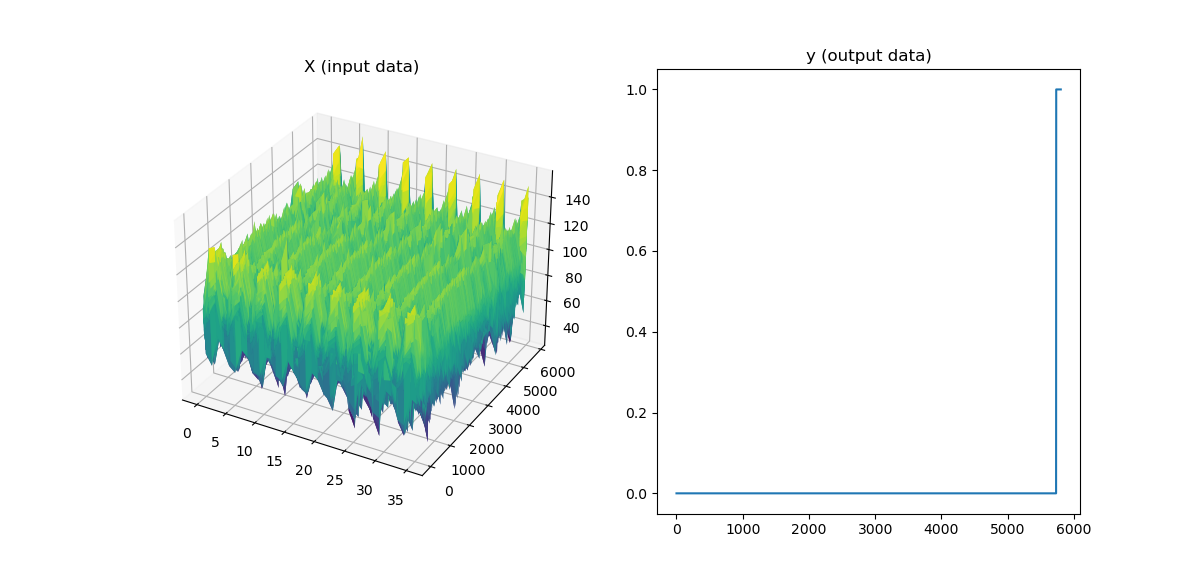
\includegraphics[width=\textwidth]{fullDataSet_mesh}
\caption{Distribution of the full data set}
\label{fig:fig1}
\end{figure}

\vspace{0.5ex}
I also examine the boxplot and volin plot (not shown) of all of the 36 attributes in the input set, but since 
the information from boxplots and voline plots are somehow repetitive and can be eye-balled from the histograms from
\texttt{pandas-profiling} in python, I decide to show only the histograms of two attributes in Figure~\ref{fig:fig2}
to provide some general information about the attribute distributions. From the histograms, I saw that most attributes
are roughly normally (as opposed to uniformly) distributed.
However, column 1, 5, 9, 13, 17, 21, 25, 29, and 33 are skewed to the right (toward higher values), but 
column 3, 7, 11, 15, 19, 23, 27, 31, 35 are skewed to the left (toward lower values).
The skewness can also be observed from the median, Q1 and Q3 quantiles in Figure~\ref{fig:fig3}.
The skewness alternates in every 4 attributes, almost as if there is a sinusoidal pattern in inlier samples.
I have also included the full report from \texttt{pandas-profiling} in the HTML format just FYI.

\begin{figure}[ht!]
\centering
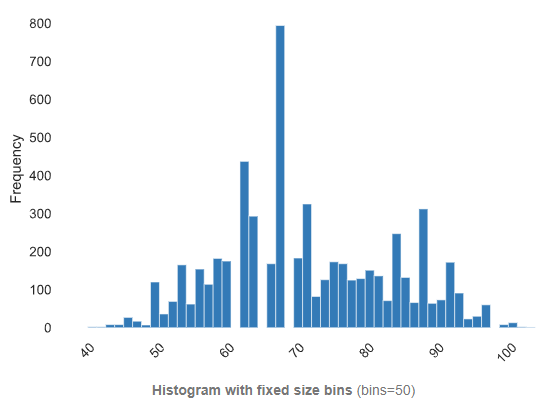
\includegraphics[width=0.48\textwidth]{boxplotAttribute1}
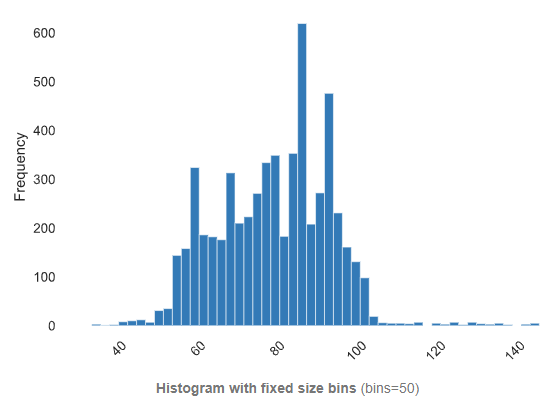
\includegraphics[width=0.48\textwidth]{boxplotAttribute4}
\caption{Distributions of the first attribute (left) and the 4th attribute (right) in the input data}
\label{fig:fig2}
\end{figure}

\pagebreak
To elaborate further on the characteristics of inliers , I show 3 different inlier samples
in Figure~\ref{fig:fig3}.
I observed that most inliers have a constant amplitude (or envelope), but the mean may vary.
The roughly constant amplitudes allow the MAC to be used for outlier detection, because MAC is
insensitive to the mean value in samples but more sensitive to the "shapes" of the samples.

\begin{figure}[ht!]
\centering
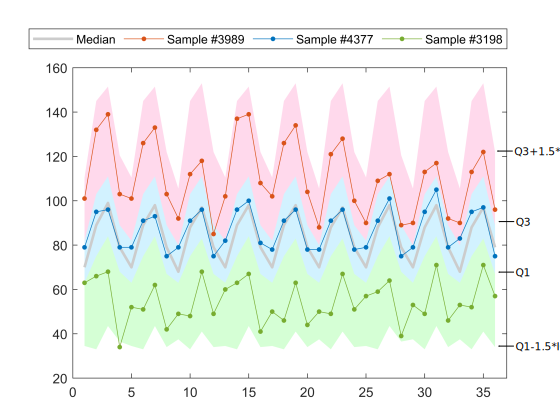
\includegraphics[width=0.75\textwidth]{inlier}
\caption{Three samples of inliers. Inliers mostly have consistent amplitudes,
although may have different mean values.
The consistent amplitudes are important feature that allow the MAC to be used for outlier detection.}
\label{fig:fig3}
\end{figure}

\vspace{1ex}
As \texttt{pandas-profiling} indicates that the data set contains only 71 outliers (2\%),
I examine all of them, and show six representative patterns in Figure~\ref{fig:fig4}.
The specific characteristics in each of the six representative samples are provided in the caption below 
Figure~\ref{fig:fig4}.
Note that the pattern difference between the inliers and outliers are interesting.
In particular, if I treated each sample as a vector, inliers' consistent amplitudes 
mean that inliers are roughly "parallel" to each other in a 36-dimensional space 
and will have MAC values close to one, whereas outliers are not parallel to the majority samples
and will have MAC values much lower than one. Therefore, in Section 4, I adopt MAC as a part of
the outlier score for outlier detection.

\begin{figure}
\centering
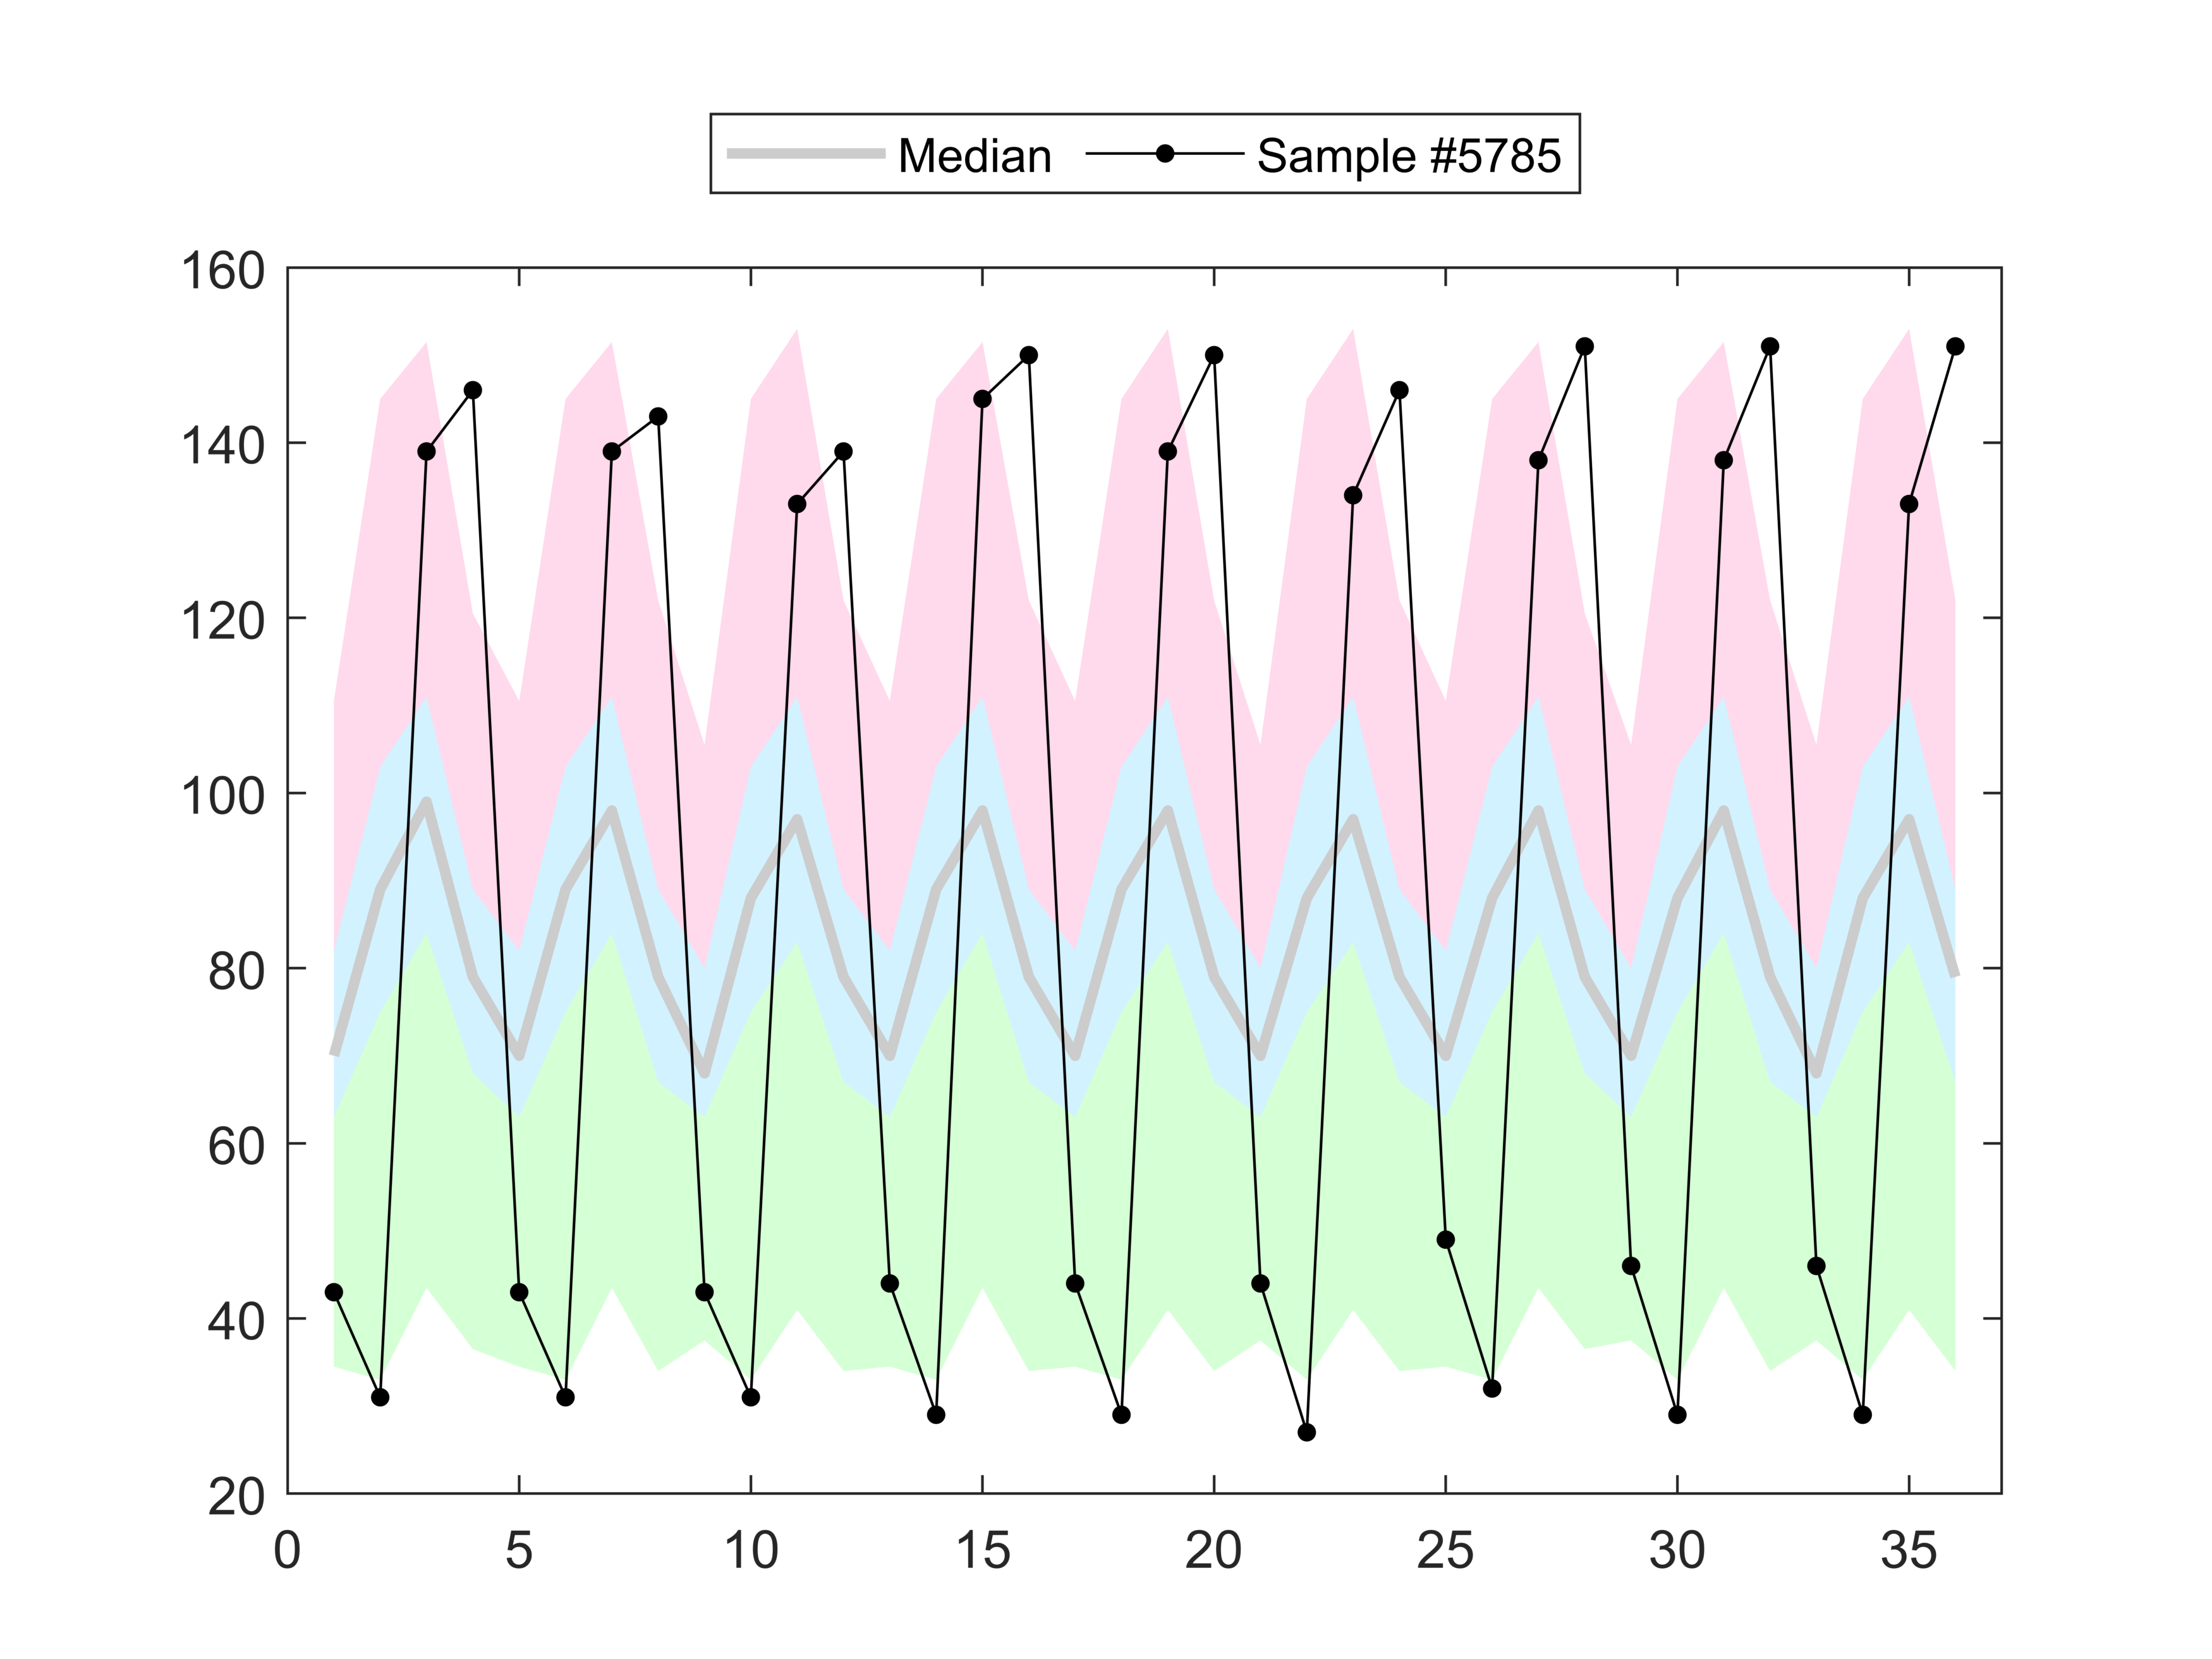
\includegraphics[width=0.48\textwidth]{outlier5785}
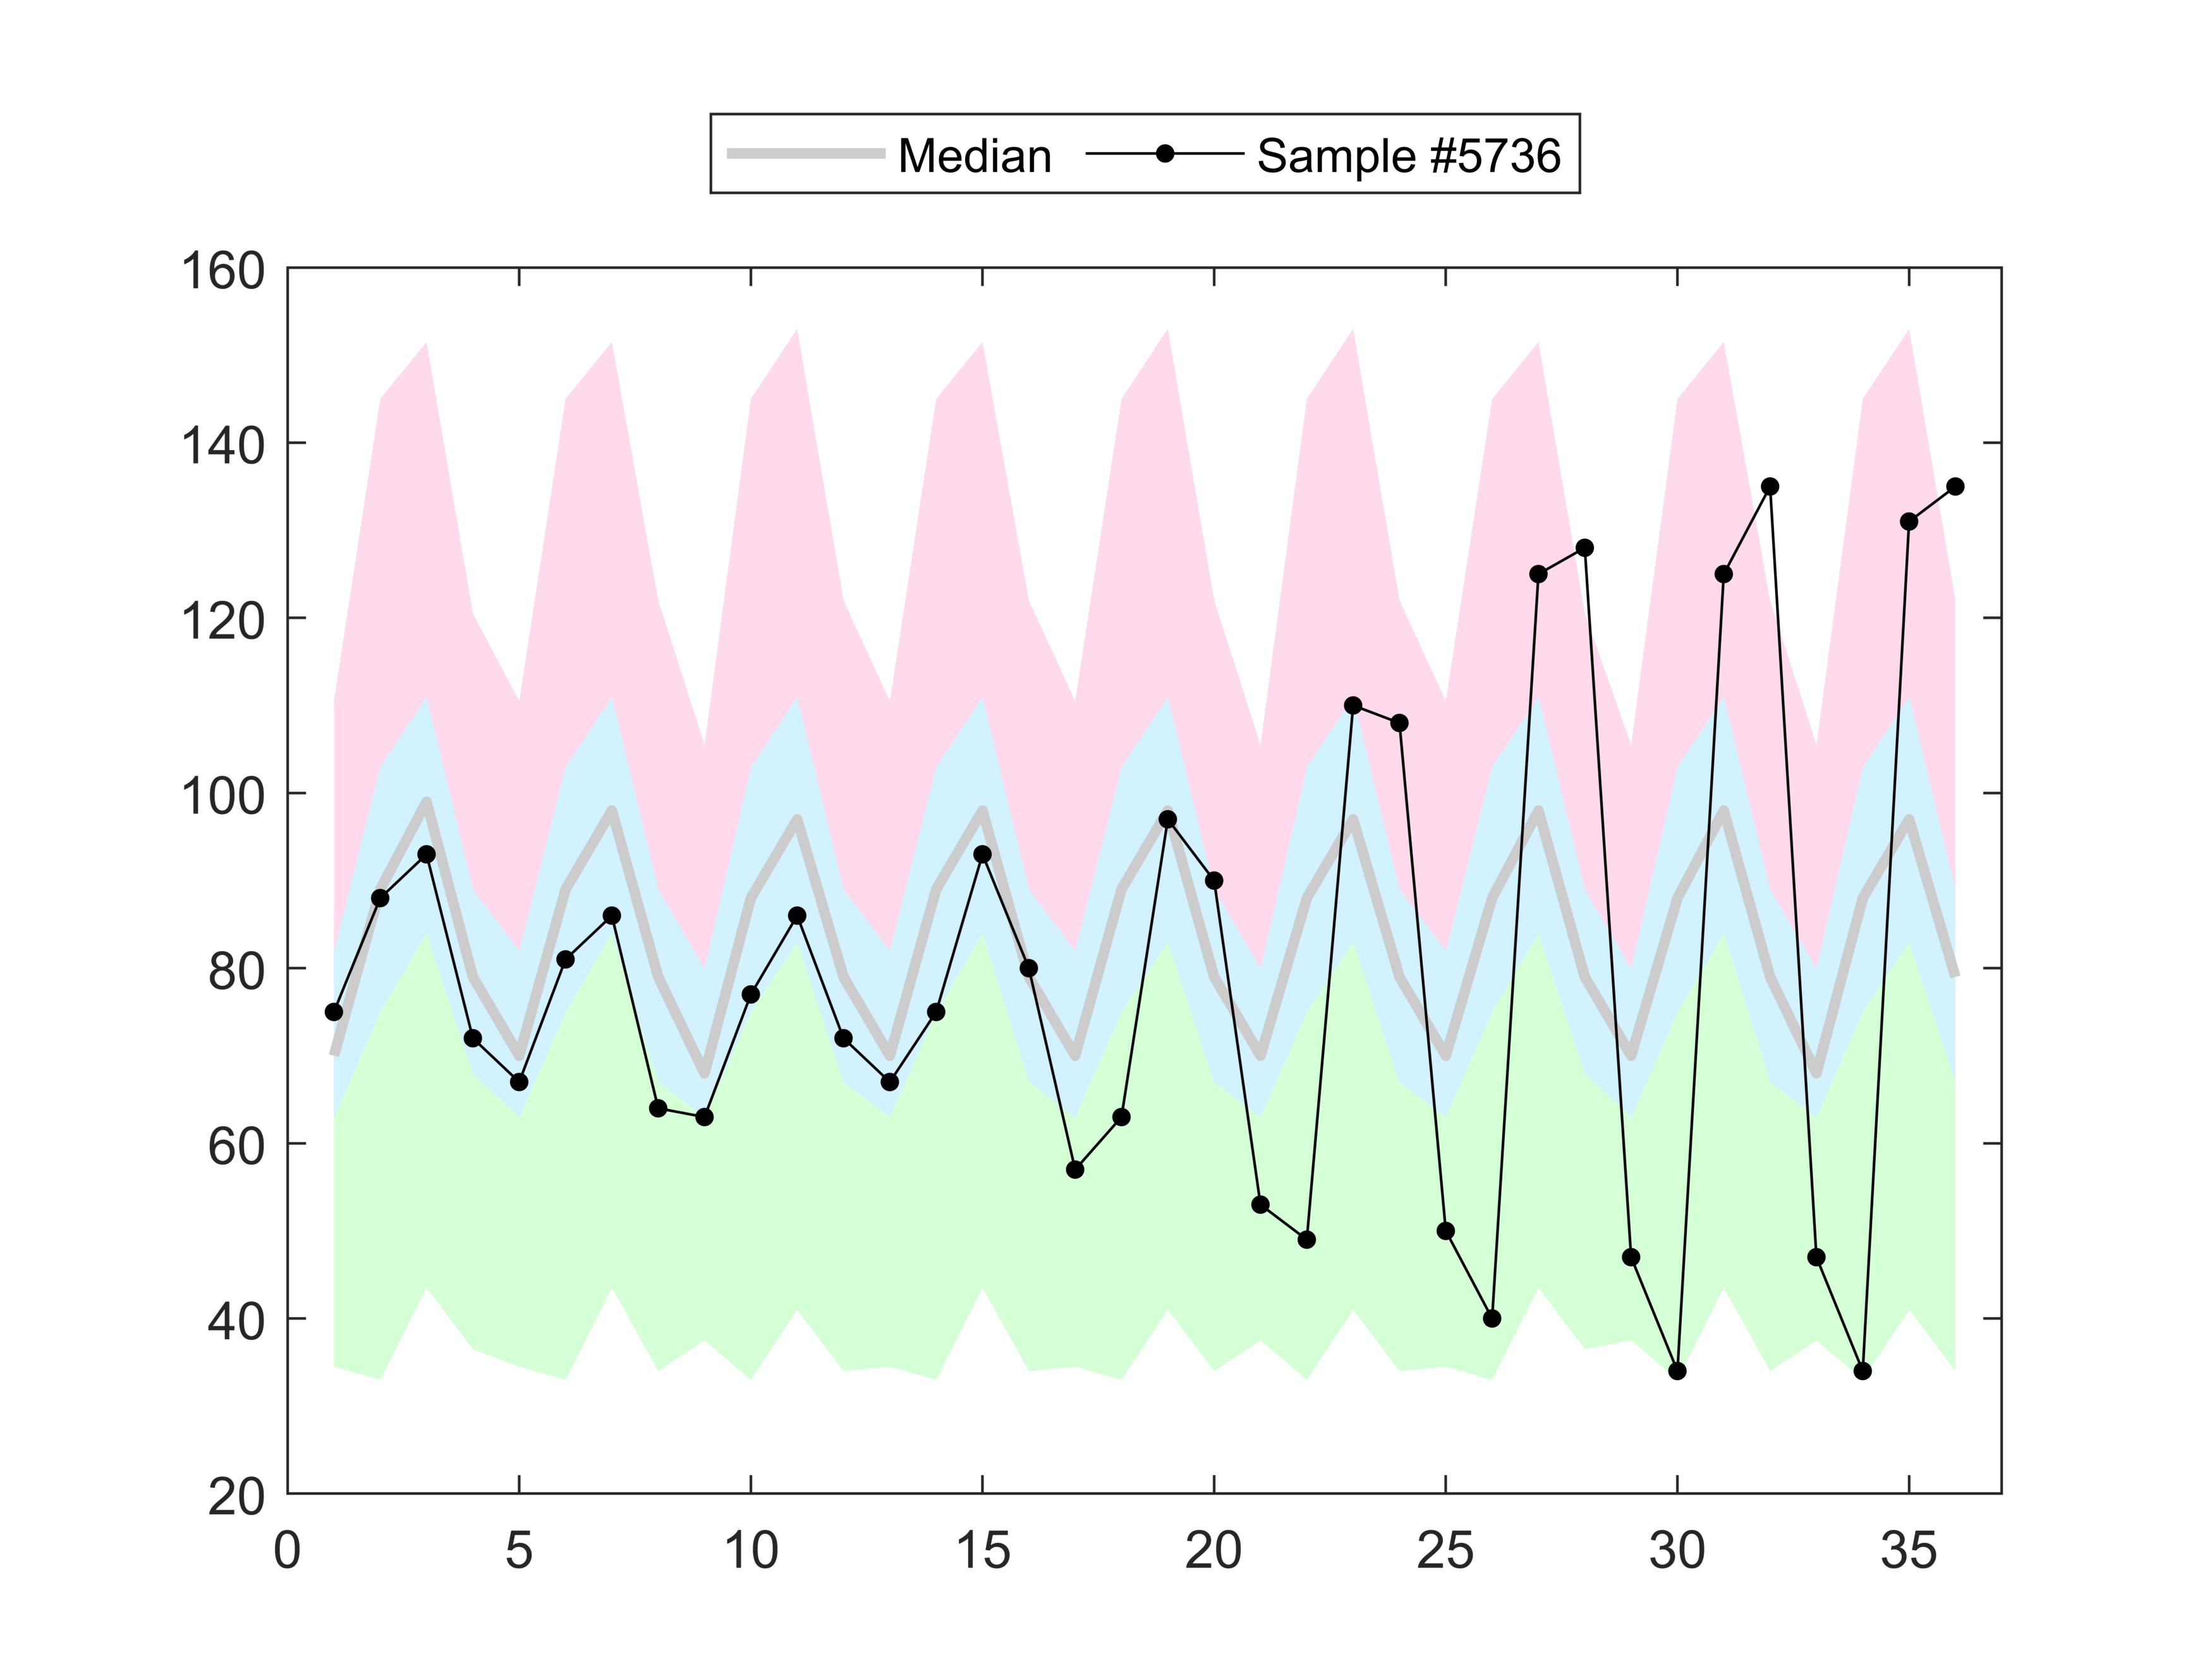
\includegraphics[width=0.48\textwidth]{outlier5736}
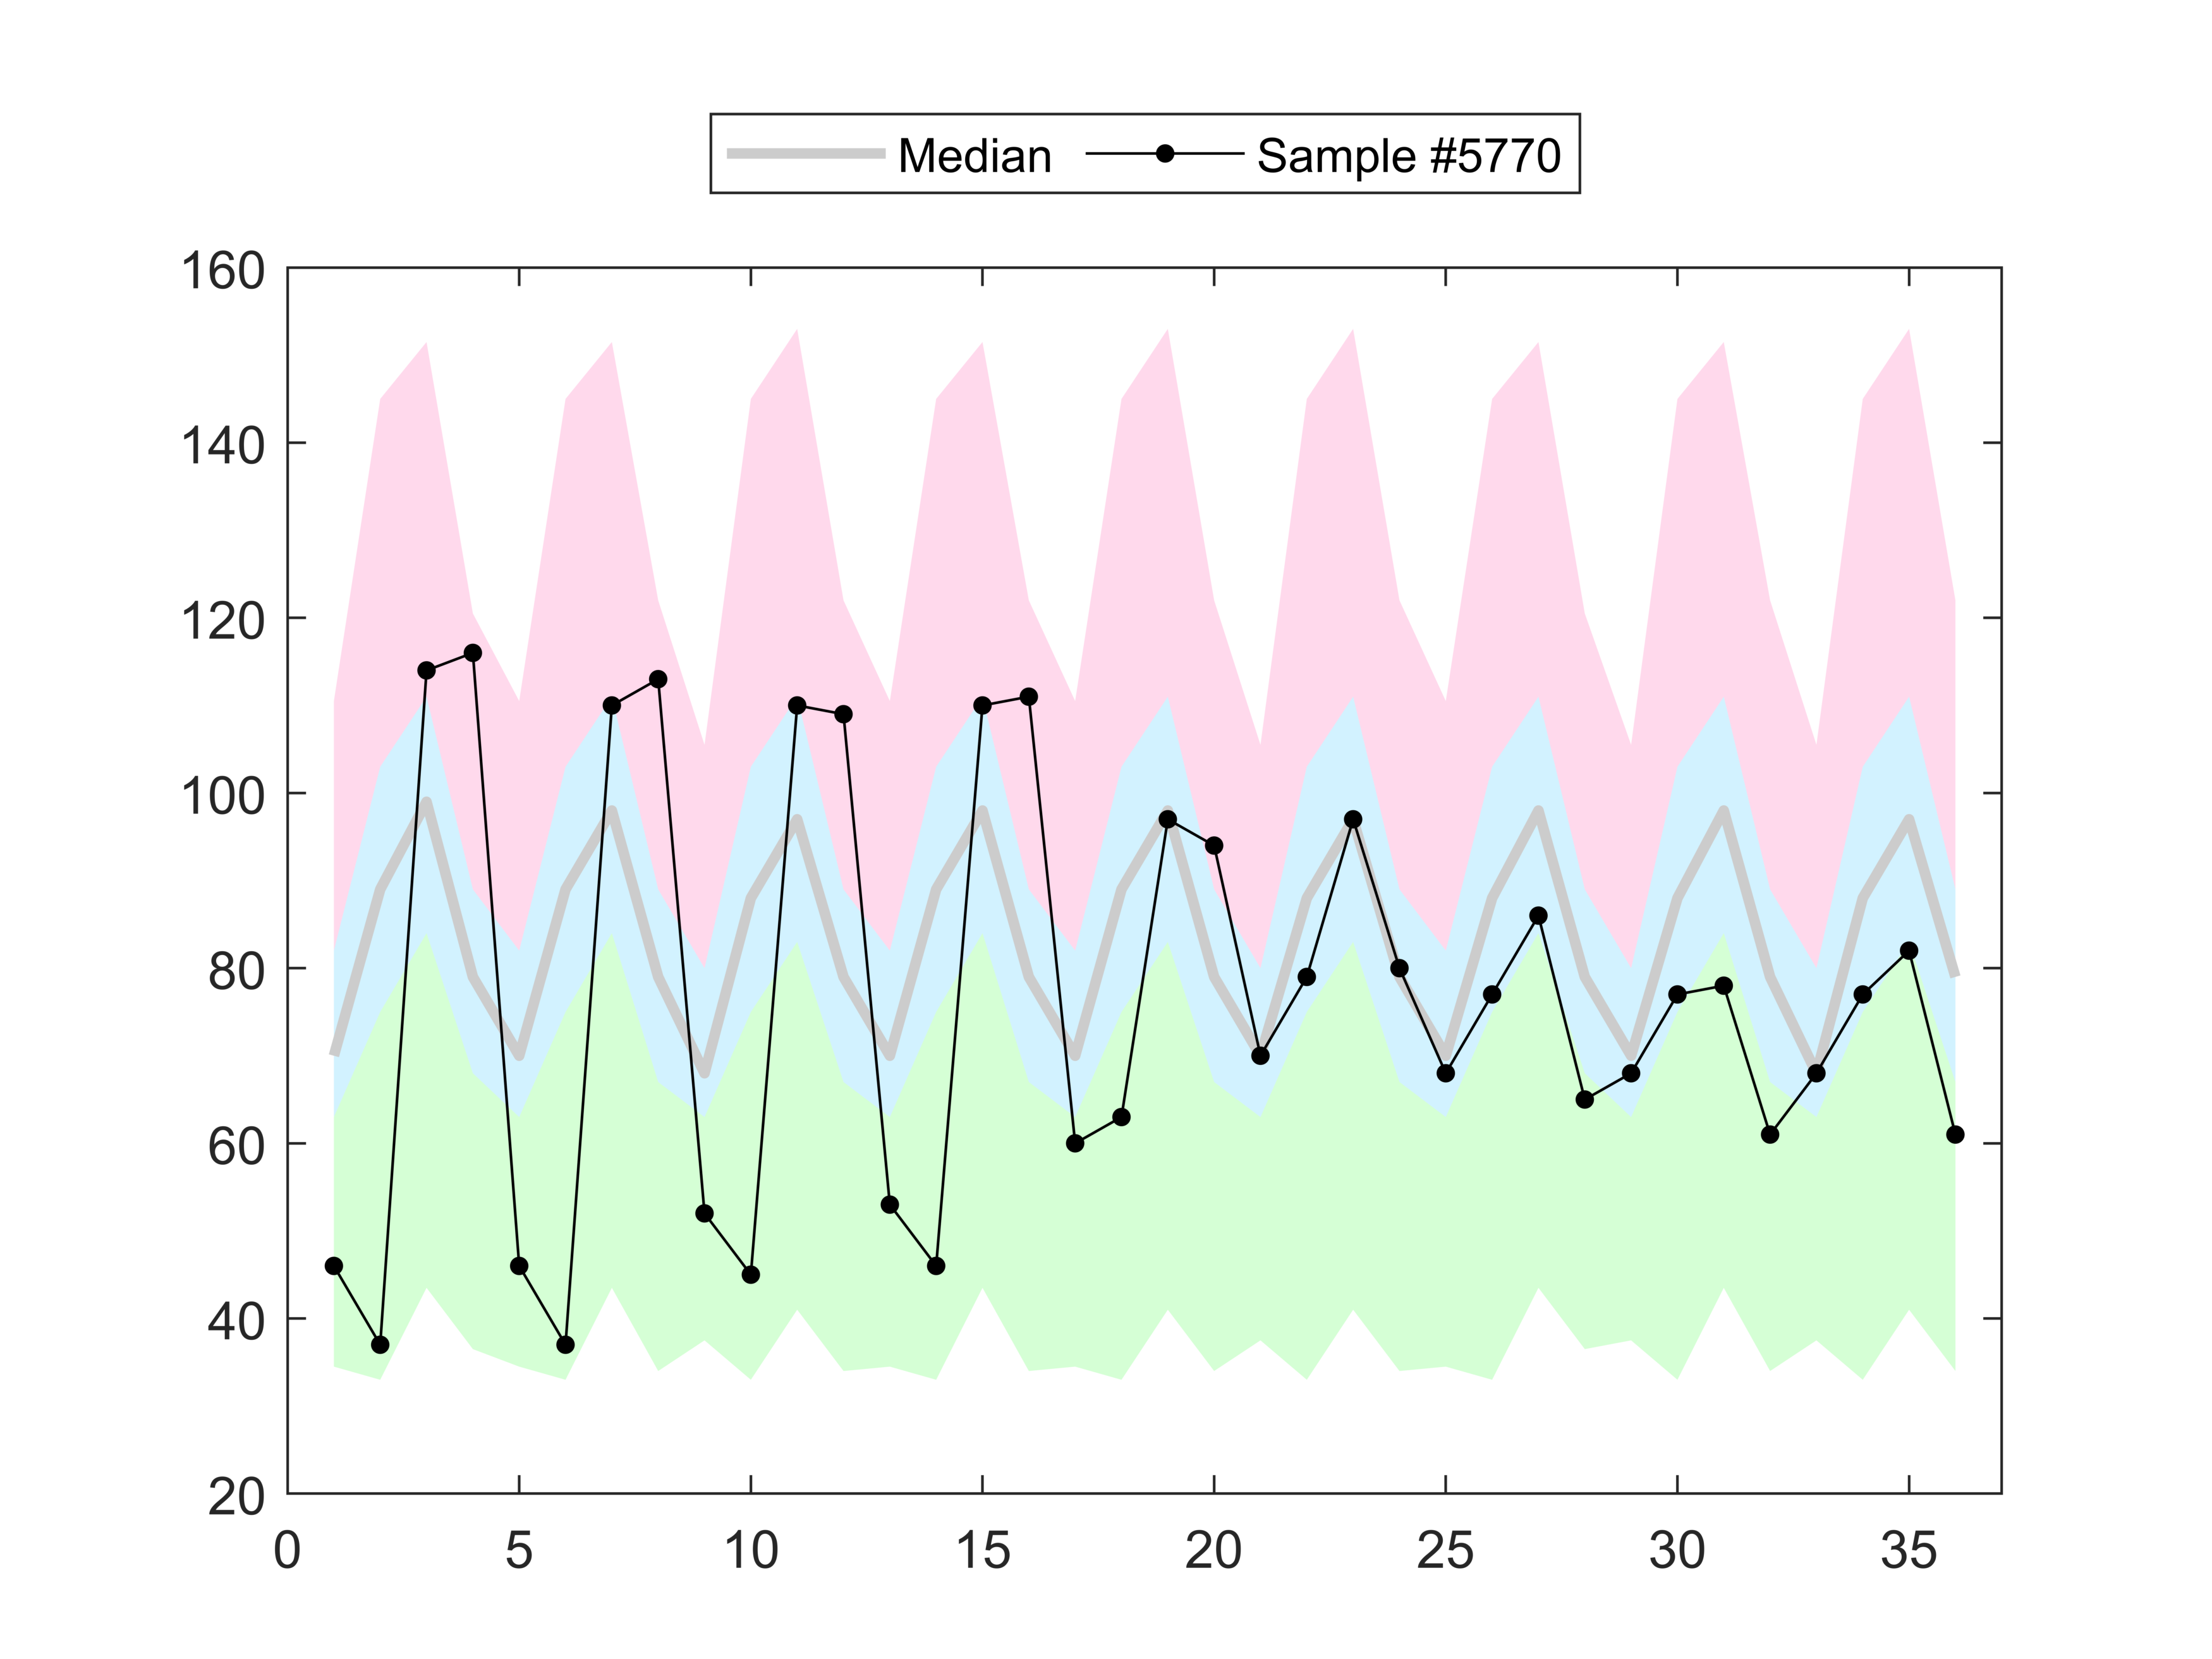
\includegraphics[width=0.48\textwidth]{outlier5770}
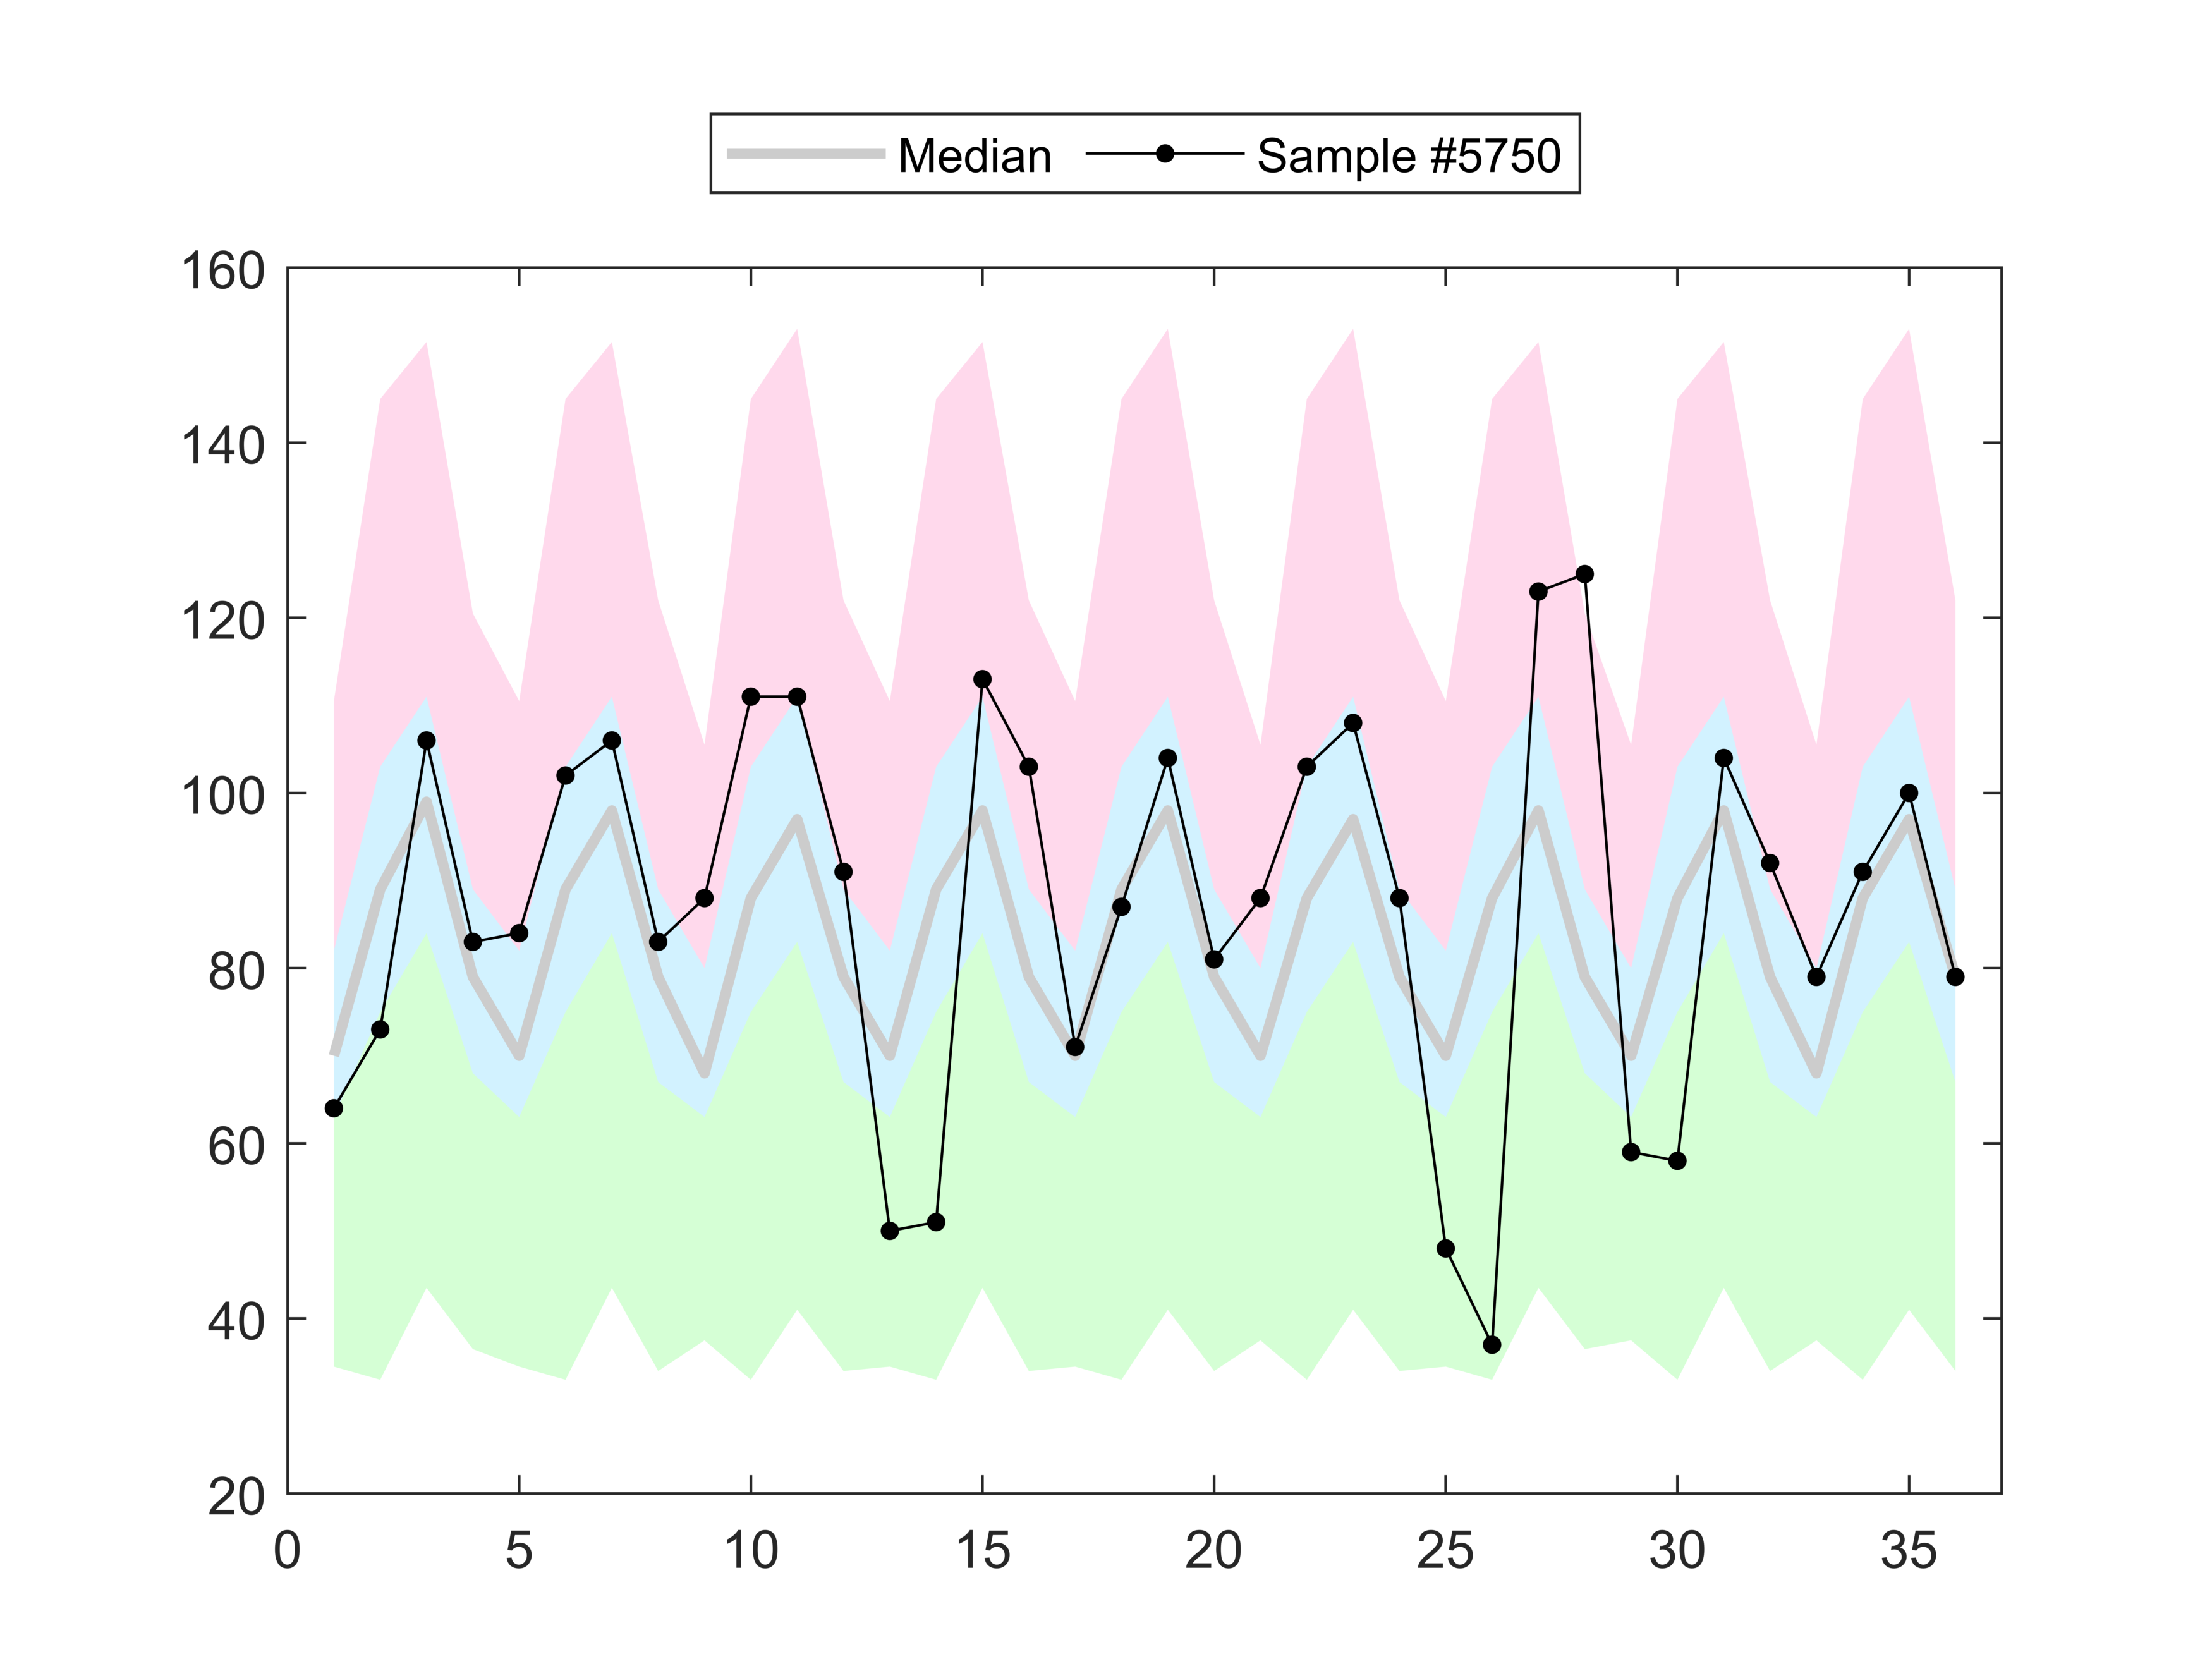
\includegraphics[width=0.48\textwidth]{outlier5750}
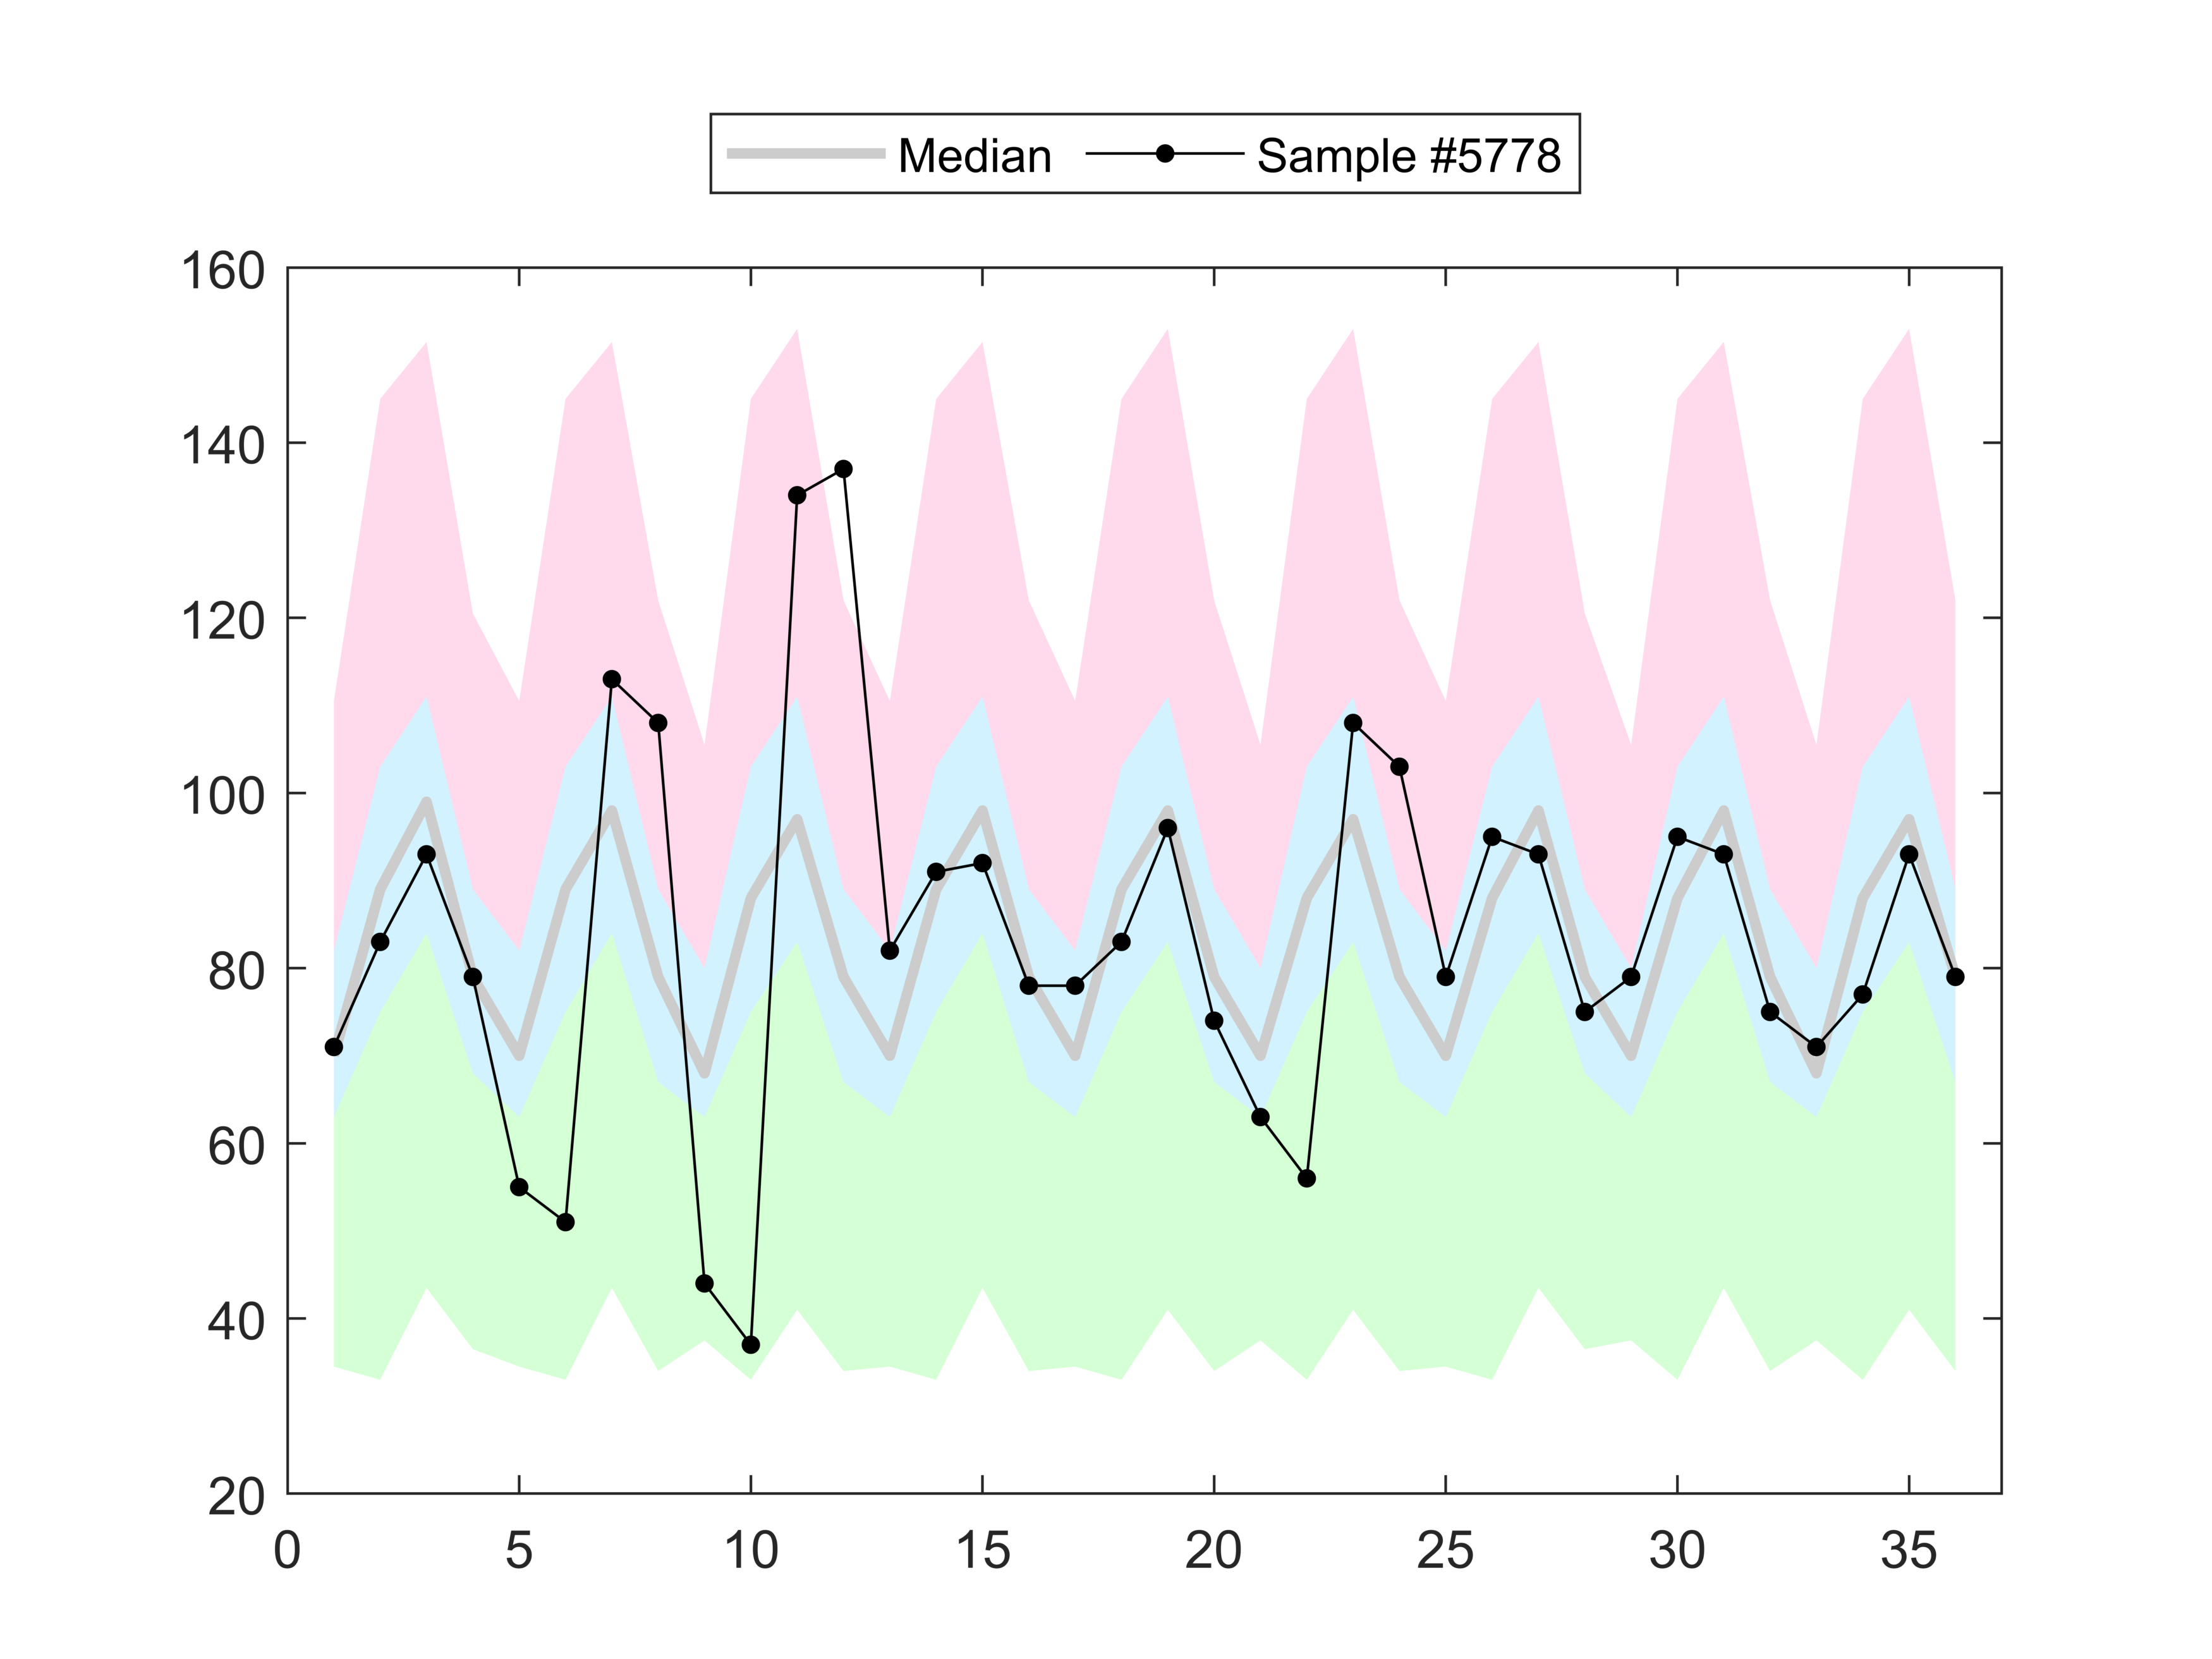
\includegraphics[width=0.48\textwidth]{outlier5778}
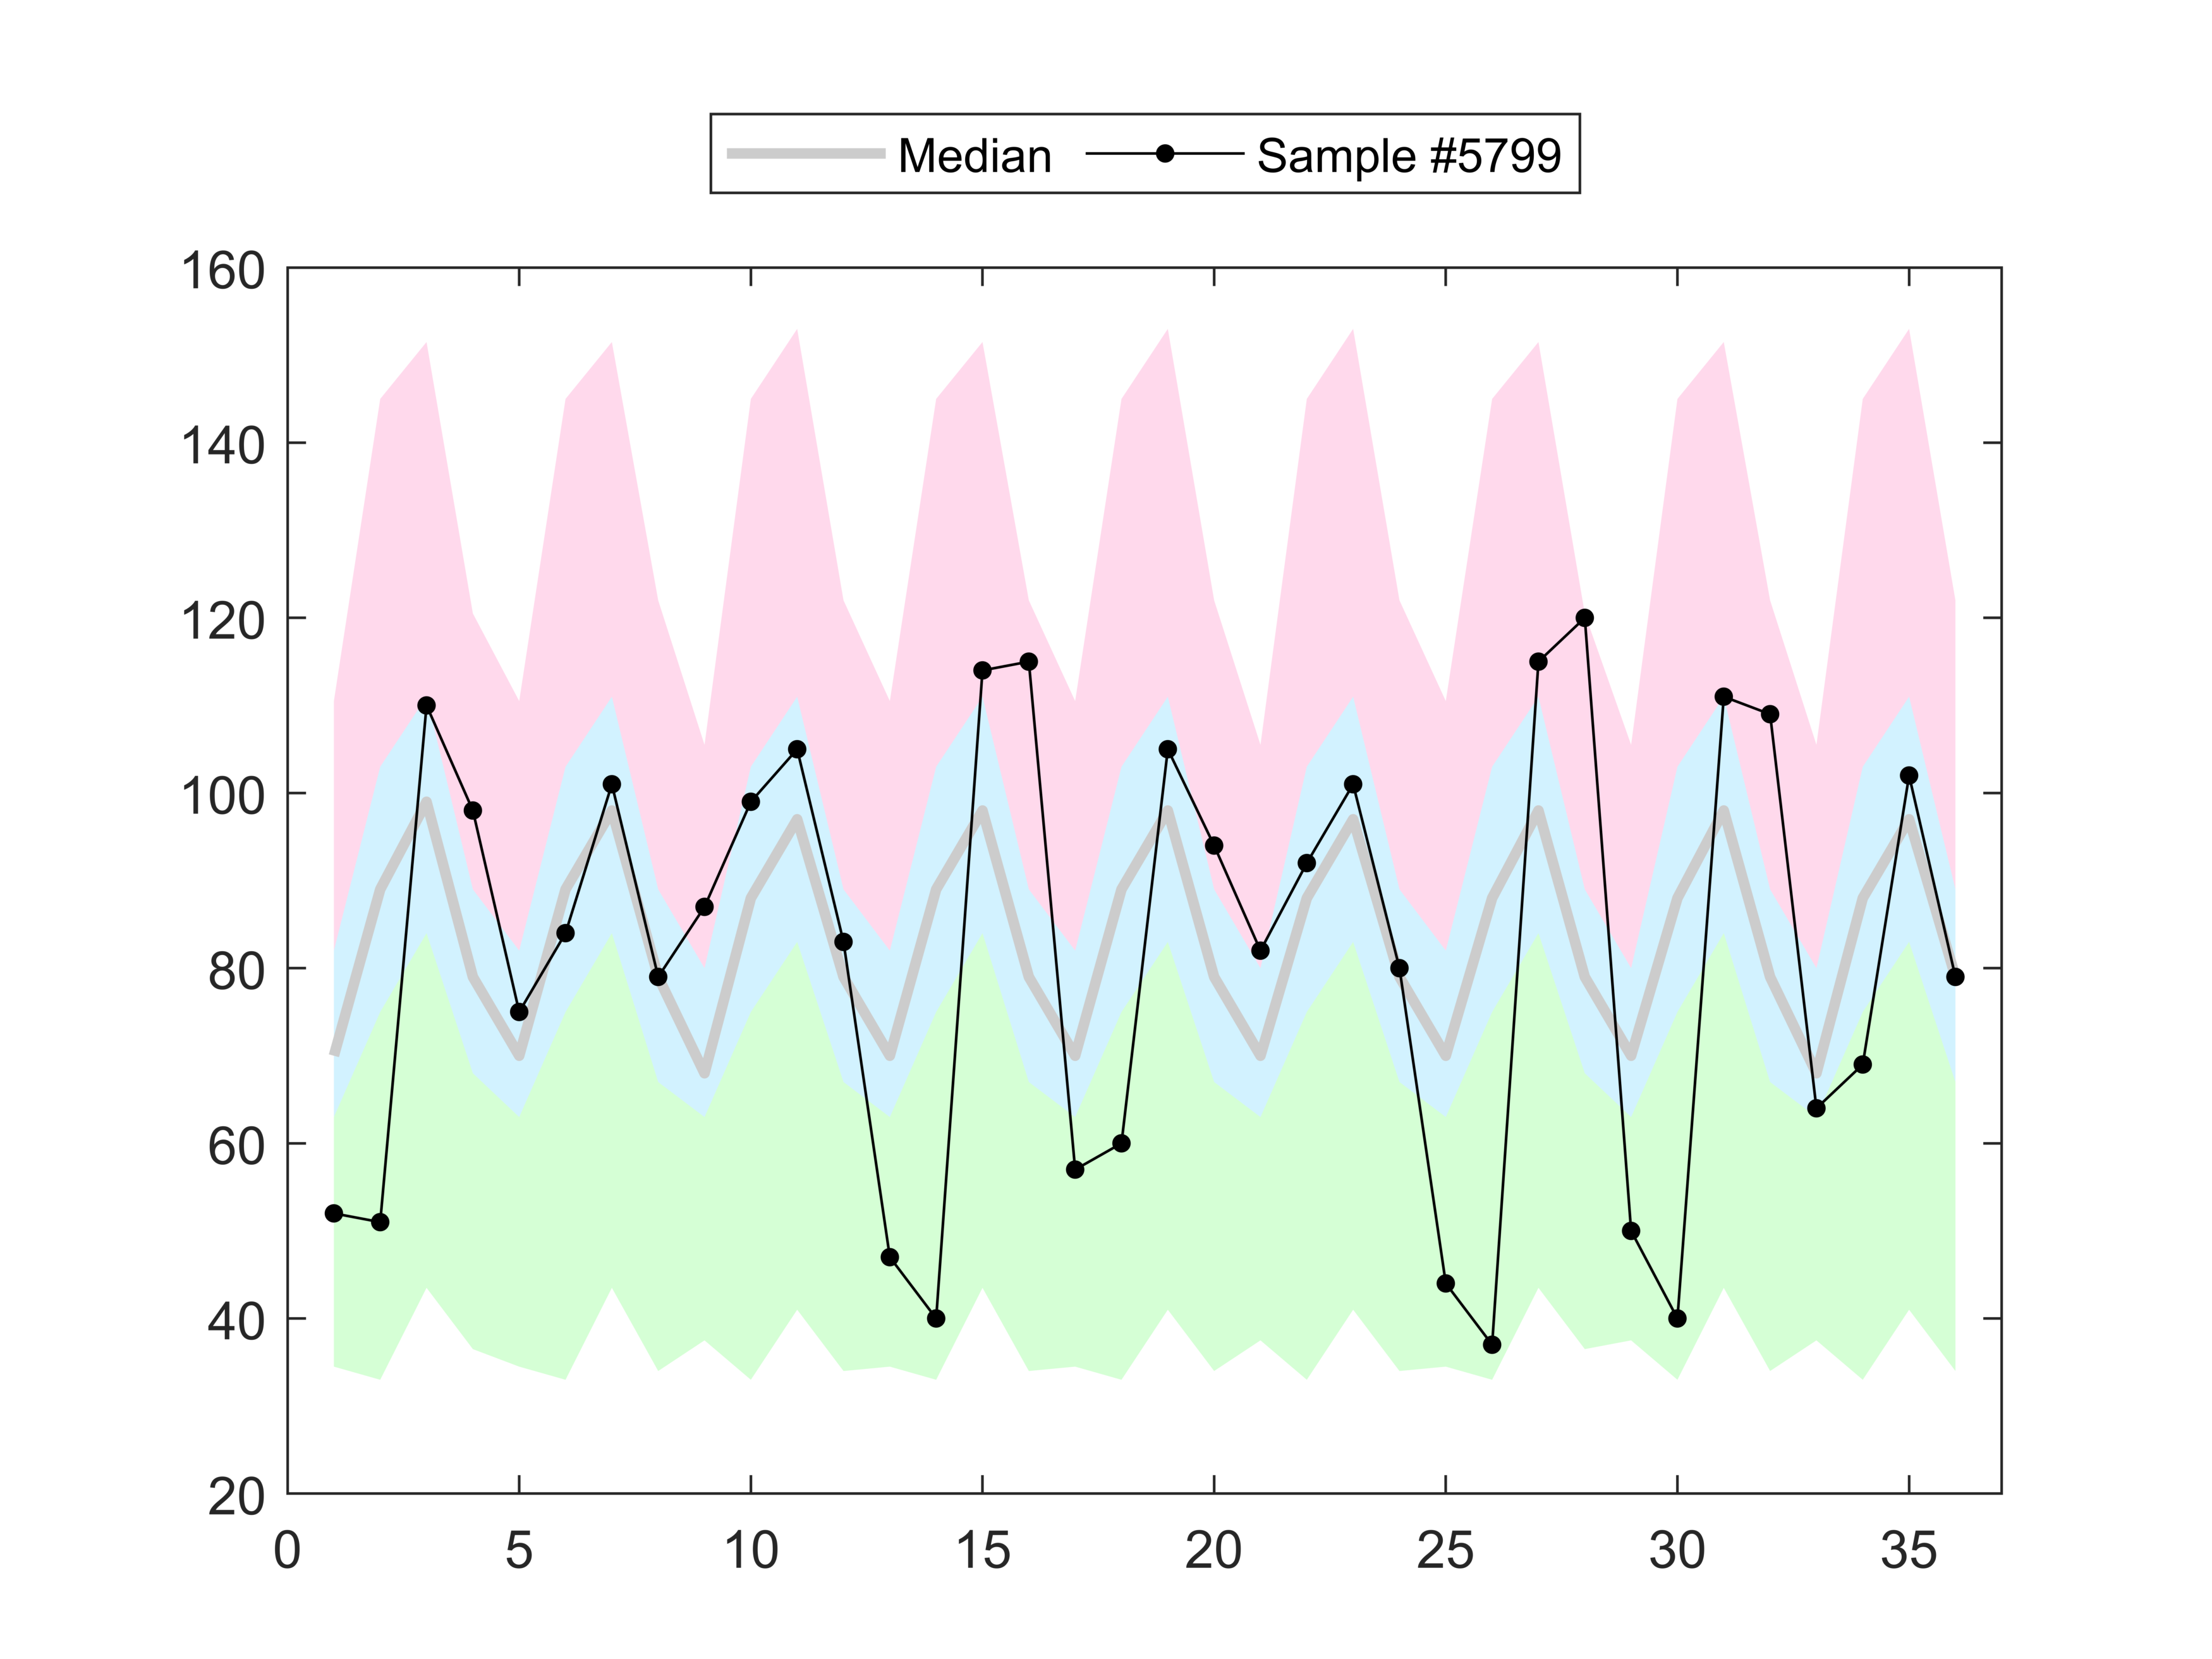
\includegraphics[width=0.48\textwidth]{outlier5799}
\caption{Six representative samples of outliers.
Top left: a sample with the amplitude fluctuating much greater then the majority;
top right: a sample with increasing amplitude;
middle left: a sample with decreasing amplitude;
middle right: a sample with sudden amplitude increases around the 25th attribute;
bottom left: a sample with sudden amplitude increases around the 13th attribute;
bottom right: a sample with irregular amplitudes.}
\label{fig:fig4}
\end{figure}

\vspace{1ex}
\section{Partial replication of Aggarwall \textit{et al.} (2005)}

In this section, I present the results of me replicating Figure 1 (d)-(f) in Aggarwall's paper.
I wrote the \texttt{my{\textunderscore}knn.m} function to calculate distances to neighbors and three wrapper scripts for varying 
the $k$ values and subsampling in \texttt{Octave}. To calcuate the ROC AUC, I adopted two 
functions, \texttt{calErr}\footnote{https://www.mathworks.com/matlabcentral/fileexchange/47364-true-positives-false-positives-true-negatives-false-negatives-from-2-matrices}
and
\texttt{roc{\textunderscore}auc}\footnote{https://www.mathworks.com/matlabcentral/fileexchange/52442-roc-curve}
, from MATLAB File Exchange;
\texttt{calErr} allows for fast calculation of True Positives, False Positives, True Negatives and False Negatives
for two matrices papulated  by 1's and 0's and \texttt{roc{\textunderscore}auc} provides guidance
of trapezoidal numerical integration for calculating the area under the ROC curve.

My result of the KNN algoirthm are shown in Figure 5-~\ref{fig:fig6}, which are consistent with Aggarwall's analysis. 
More specifically, Figure 5 has shown the strength of numbers in a intuitive way, in that the outliers in the
\texttt{satimage-2} data set are not particular hidden, the performance of KNN algorithm improves when more neighbors are called
up to help identifying the outlier.
Aggarwall's argument on the bias reduction and variance reduction are also correctly replicated in the left and right panels 
in Figure \ref{fig:fig6} respectively, in which I use almost identical settings a Aggarwall's with 100 trails to obtain the
performance distributions of KNN with subsampling.

I did not proceed to implement the variable subsampling proposed by Aggarwall as I believe their arguments are logical and accurate.

\begin{figure}[ht!]
\centering
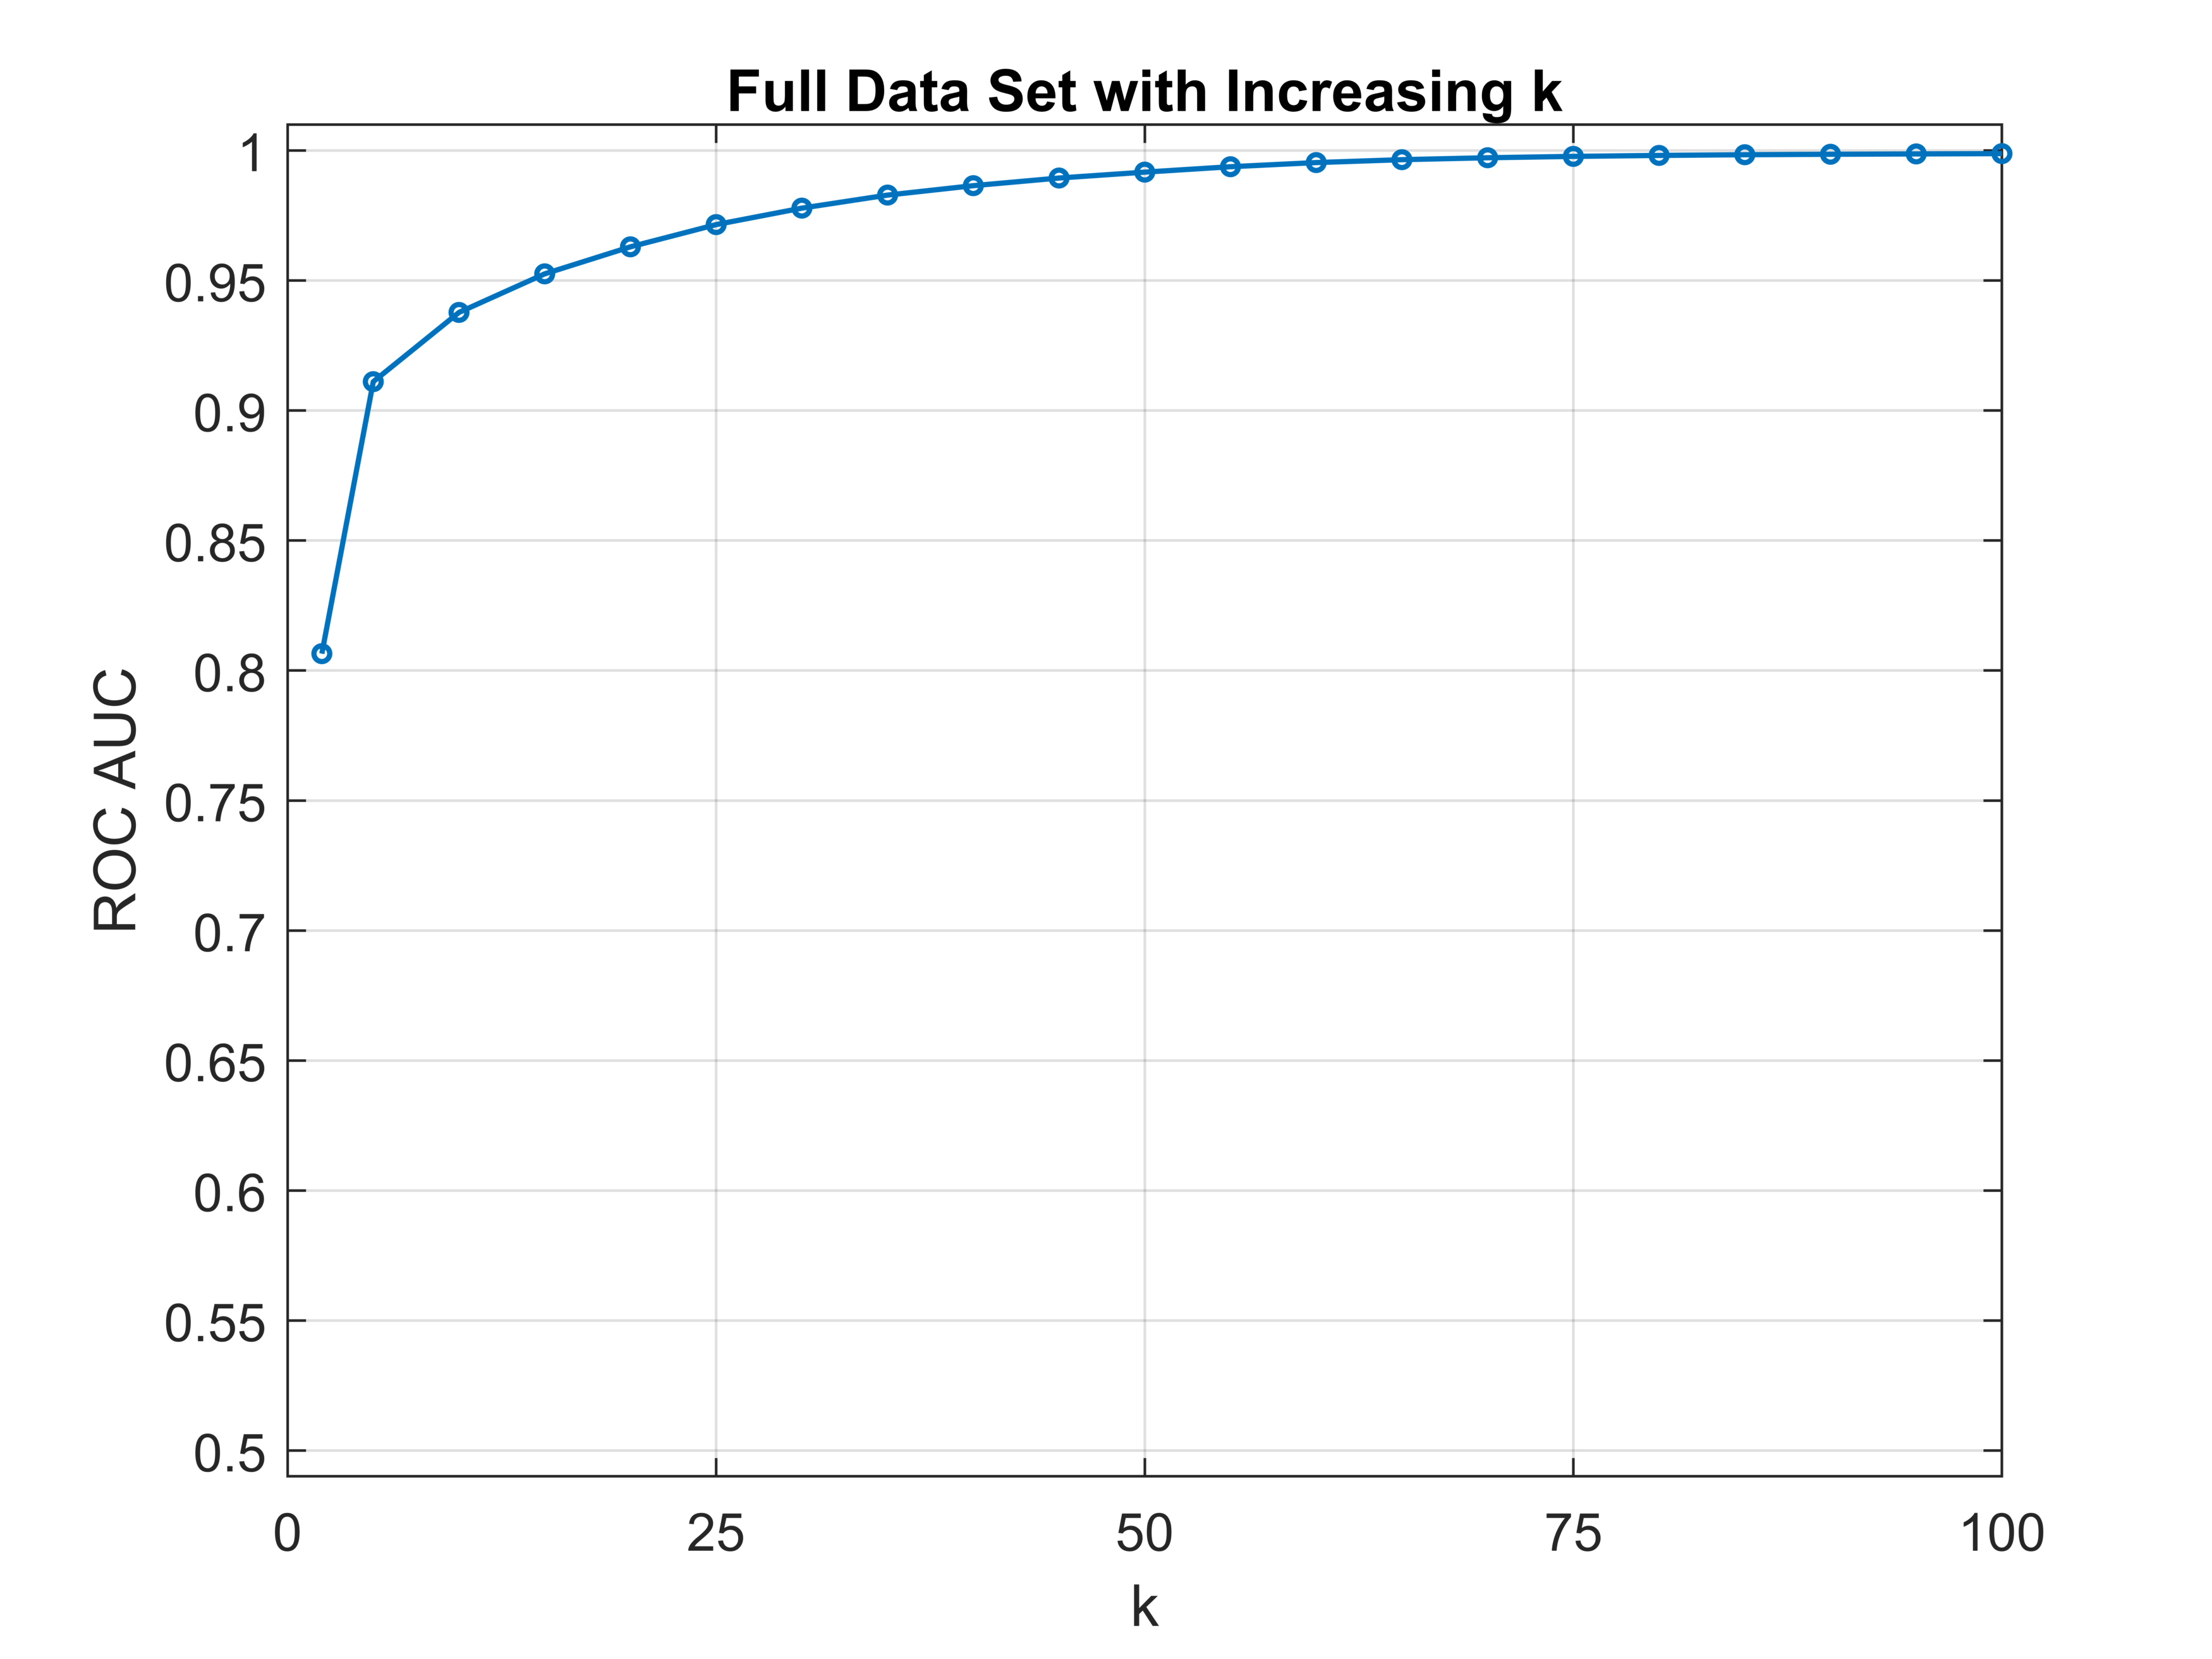
\includegraphics[width=0.55\textwidth]{fullDataSet_increasingK}
\caption{Performance of the KNN algorithm using the full data set with increasing $k$.}
\label{fig:fig5a}
\end{figure}

\begin{figure}[ht!]
\centering
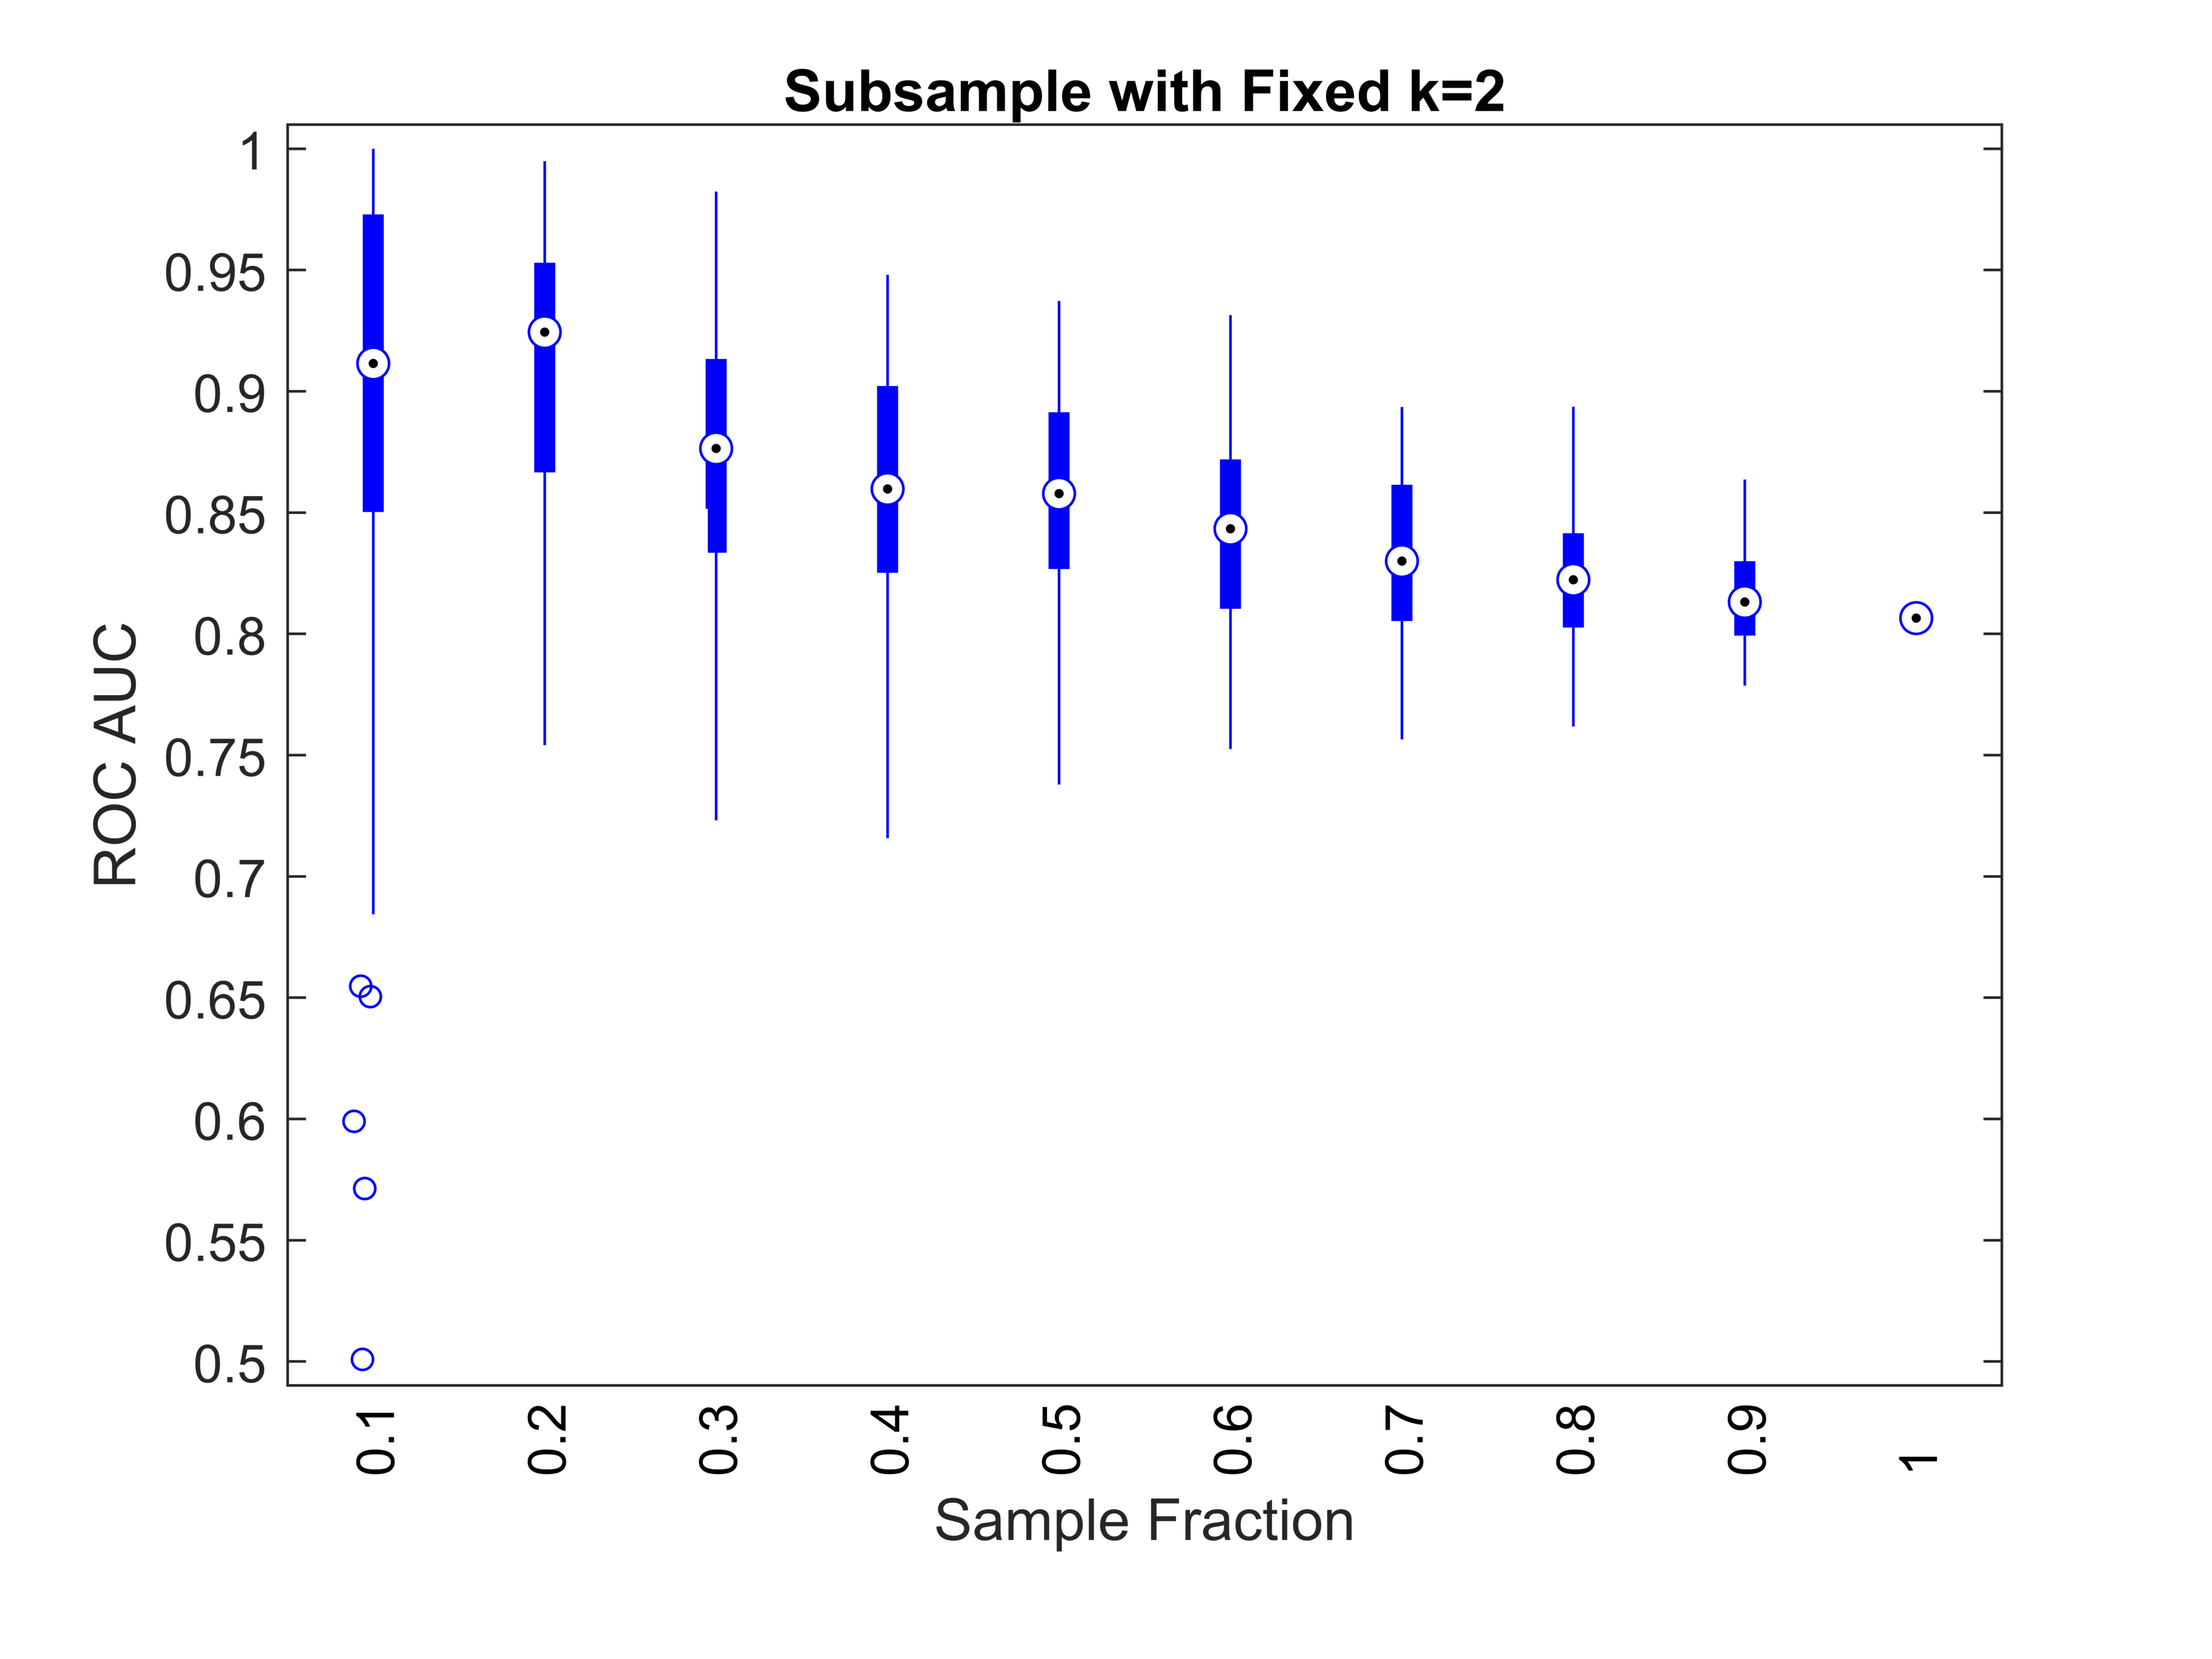
\includegraphics[width=0.48\textwidth]{subsampleWithFixedK}
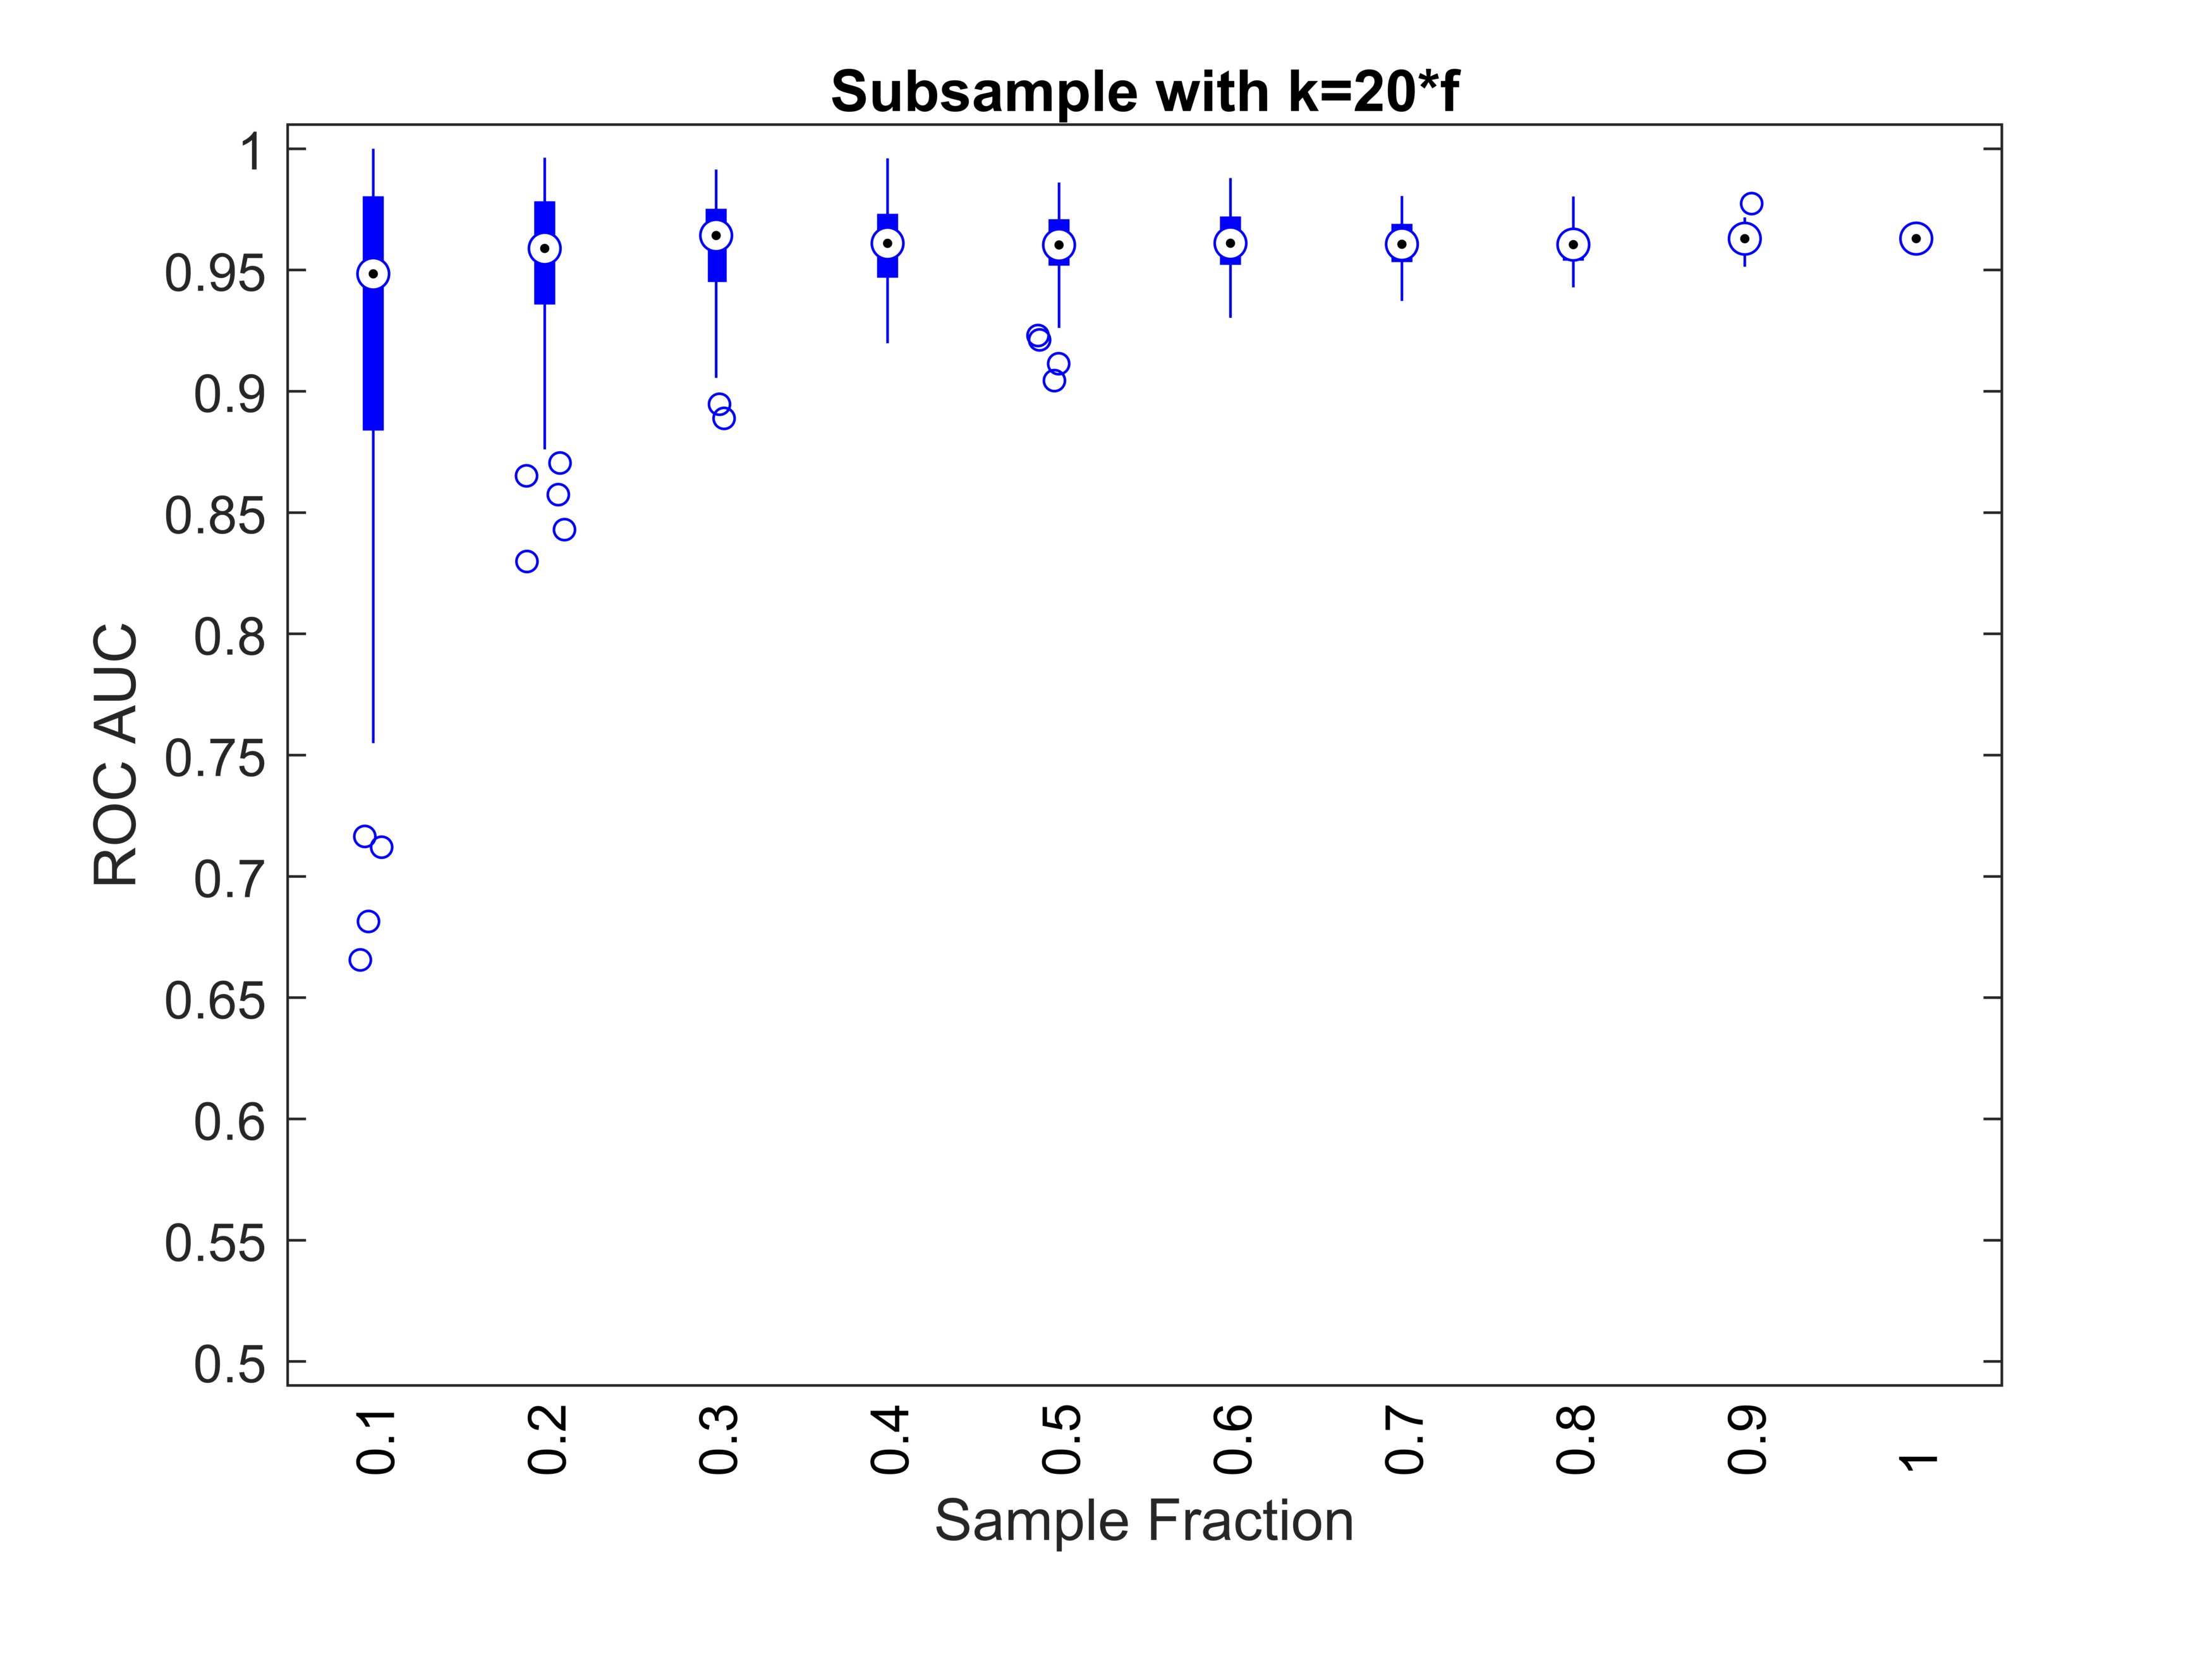
\includegraphics[width=0.48\textwidth]{subsampleWithProportionalK}
\caption{Performance of the KNN algorithm with subsampling. Left: Subsampling with $k=2$ (fixed) and $k=20f$ (right).}
\label{fig:fig6}
\end{figure}

\vspace{10ex}
\section{My algorithm based on MAC for outlier detection}
I borrowed the modal assurance criterion (MAC) in experimental modal analysis to create an algorithm
for outlier detection.
The MAC is defined as the normalized scalar product of two sets of vectors $\Phi_A$ and $\Phi_X$,
and always takes a value within $0\mbox{-}1$.
The resulting scalars are arranged into the MAC matrix:
\begin{gather*}
MAC(i,j) = \dfrac{|\phi_{i}^T\phi_{j}|^2}{\left(\phi_i^T\phi_i\right)\left(\phi_j^T\phi_j\right)}
\; \; , \,
\phi_i \in \Phi_A
\; \; , \,
\phi_i \in \Phi_X
\end{gather*}

In the above formula, MAC will be 1 when $\phi_{i}$ and $\phi_{j}$ are aligned (i.e. parallel) to each other.
In other words, MAC will be 0 when $\phi_{i}$ and $\phi_{j}$ are orthogonal (i.e. completely misaligned) to each other.
Note that MAC can work with vectors with different length because of the normalization in the denominator;
therefore, it takes care of the situation in Figure 3 when inliers have the same shape but different mean values
(i.e. \textit{directionally} aligned in a multi-dimensional space but with offsets).

MAC is traditionally used to compare if the mode shapes between a model and an experimental data are consistent;
similar comparison can also be made among two models or even two experimental data sets.
However, here I am using MAC to evaluate if vectors are similar to each other \textit{within} the same set; in other words,
I am making $\Phi_A$ identical to $\Phi_X$. Furthermore, for outlier detection, I flip the MAC by the following formula, such that the output will take a larger value
when a vector $\phi_i$ is more different than all other $\phi_j$. I then sum the columns in the MAC matrix to obtain a row vector as the outlier score.
For example, Figure~\ref{fig:fig7} and 8 shows two examples with 20 and 50 samples from the \texttt{satimage-2} data set.
I adopt the \texttt{mac}\footnote{https://www.mathworks.com/matlabcentral/fileexchange/53173-modal-assurance-criterion-mac} function on MATLAB file exchange to facilitate the MAC calculation. 

\[
\text{Output}(i,j) = 1 - MAC(\phi_i,\phi_j)
\]

\[
\text{Outlier score}(j) = \sum_i \text{Output}(i,j)
\]

From the preliminary results in Figure 7 and 8, I further revise and normalize the outlier score by the sample size,
such that an universal threshold for outlier detection may be used when the sample size changes:
\[
\text{Normalized outlier score}(j) = \dfrac{{\sum}_i\left(1 - MAC(\phi_i,\phi_j)\right)}{\text{sample size}}
\]

Since the data set is roughly normally (as opposed to uniformly) distributed and the outliers are not hidden,
choosing a threshold is fairly easy. This particular data set has inliners scored around 0.02 (after normalization; see Figure 9-12) and outliers 
scored arbitrarily higher. Therefore, I choose 0.1 as the threshold and test if the algorithm can be scaled up and down.
The simulations on various sample sizes are shown in Figure 9-12 with the f1 score printed in the title.

\begin{figure}[ht!]
\centering
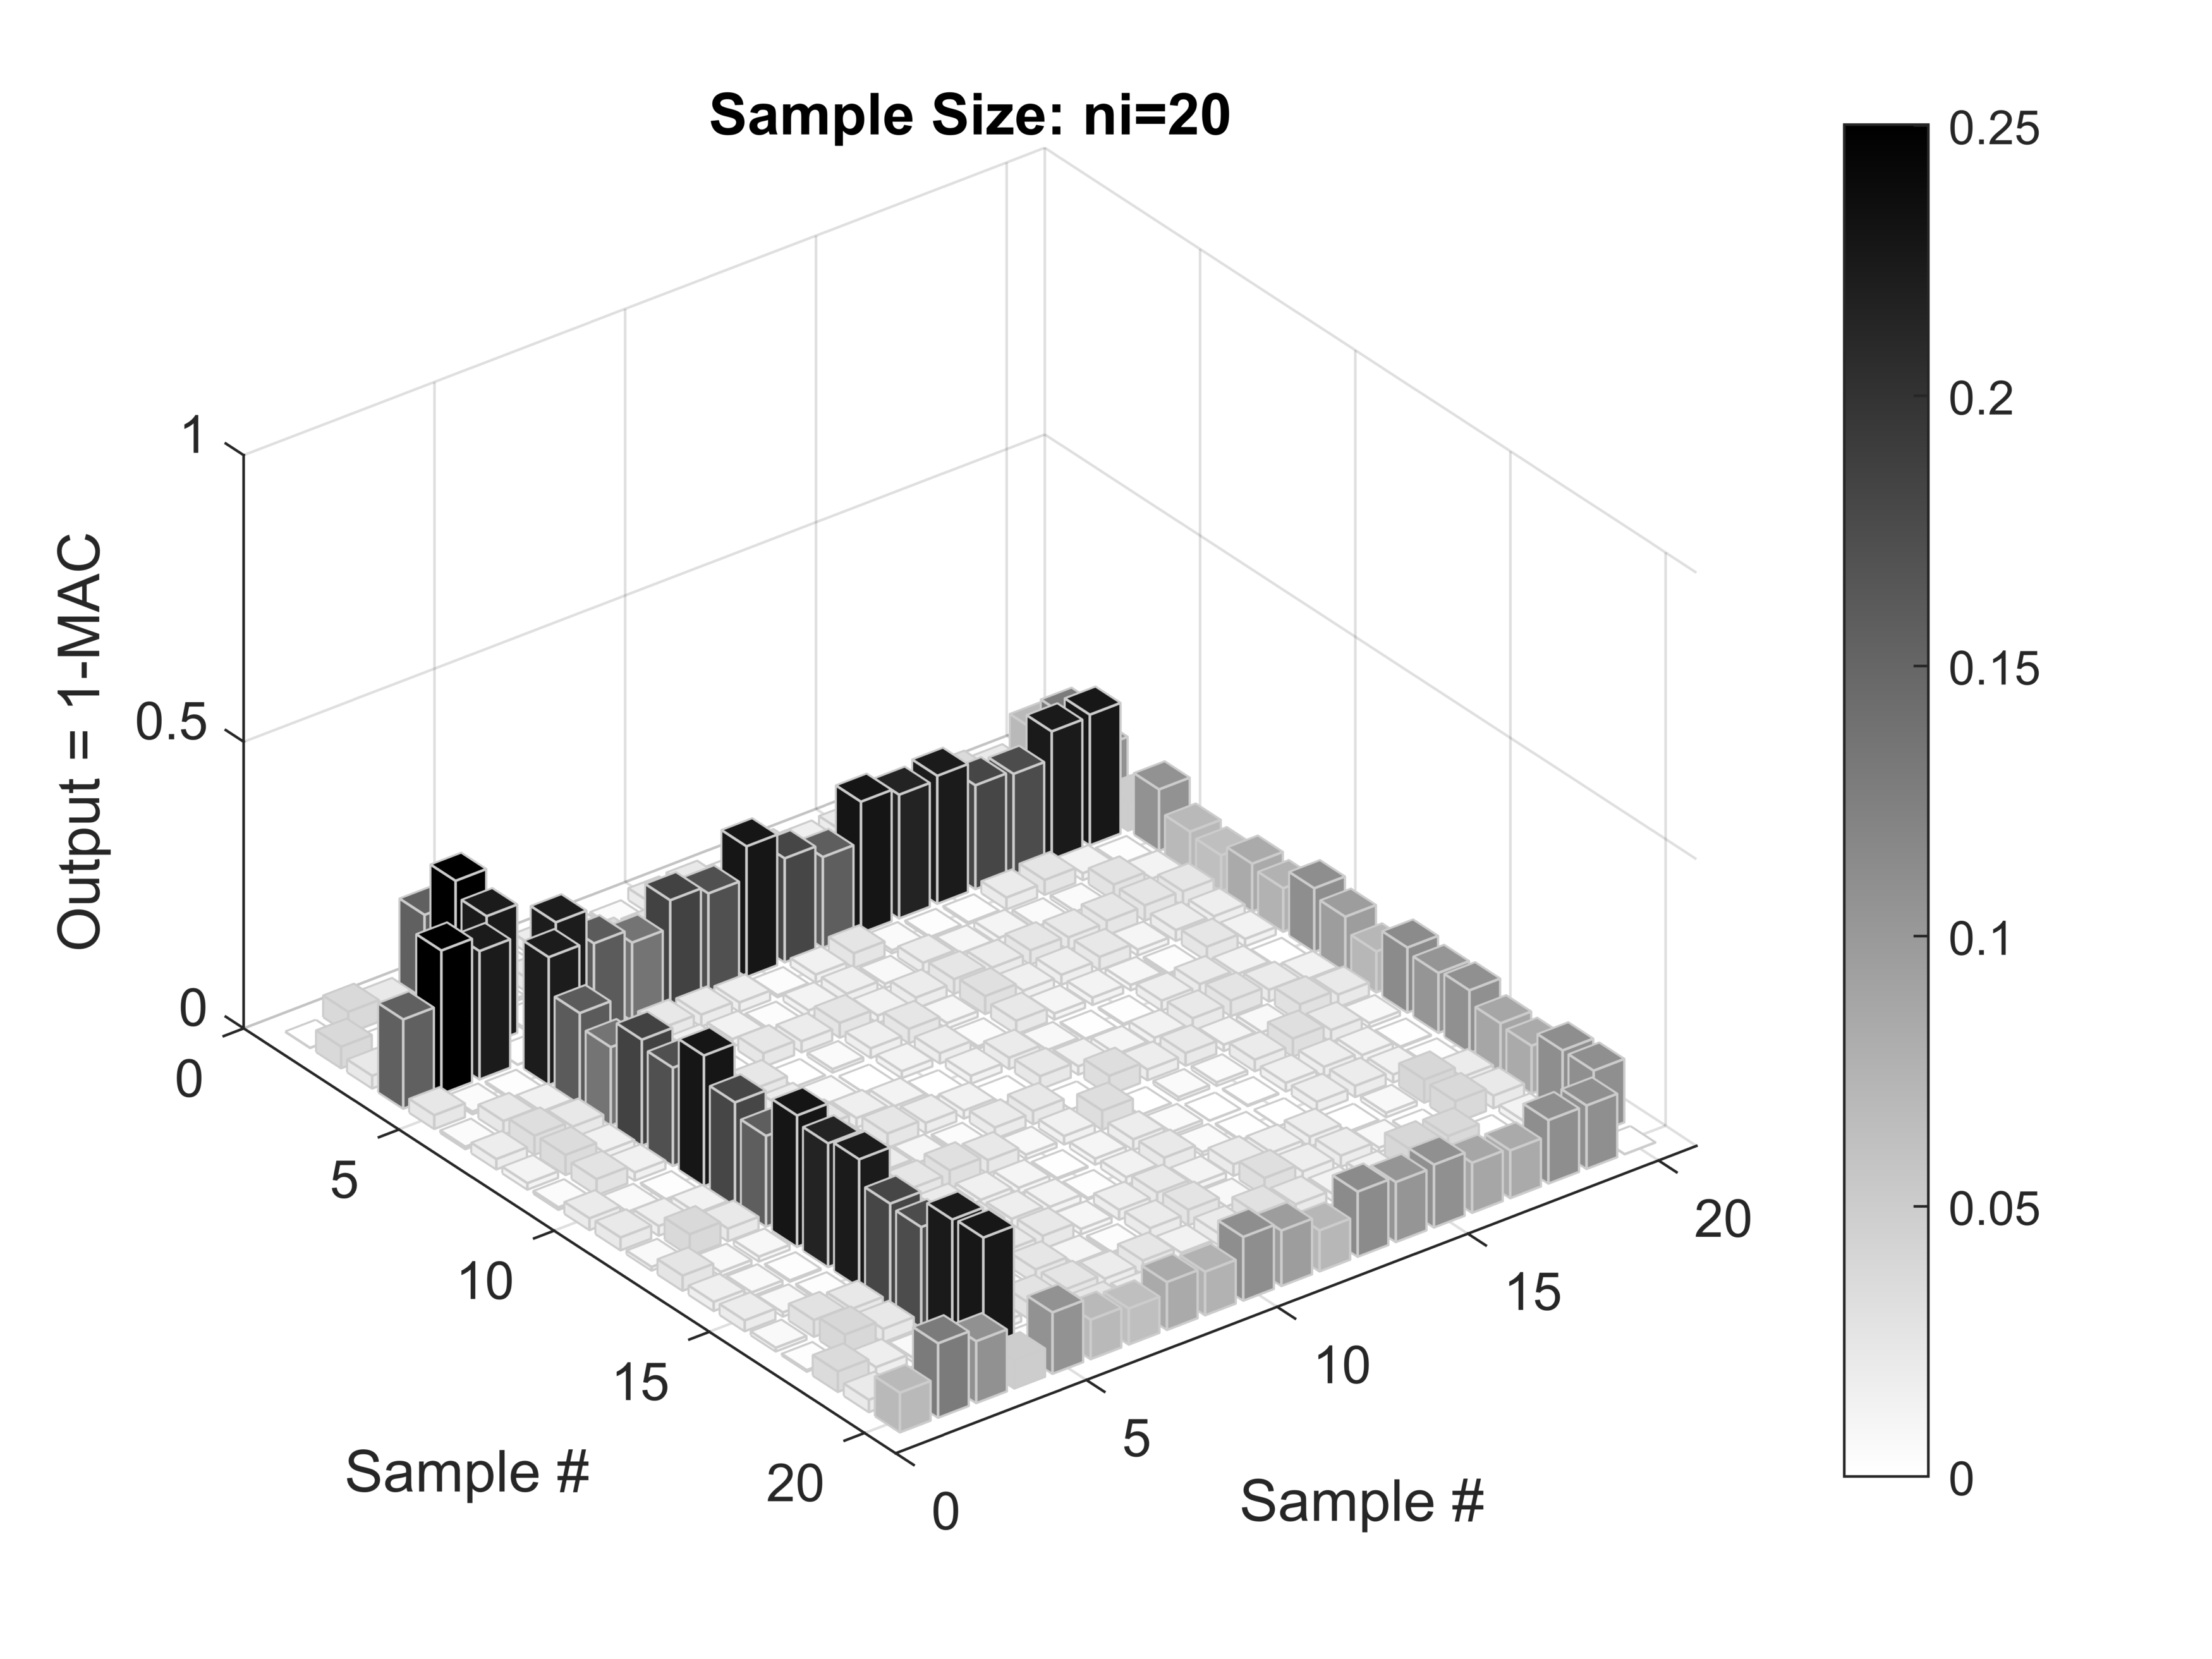
\includegraphics[width=0.48\textwidth]{MAC_ni20}
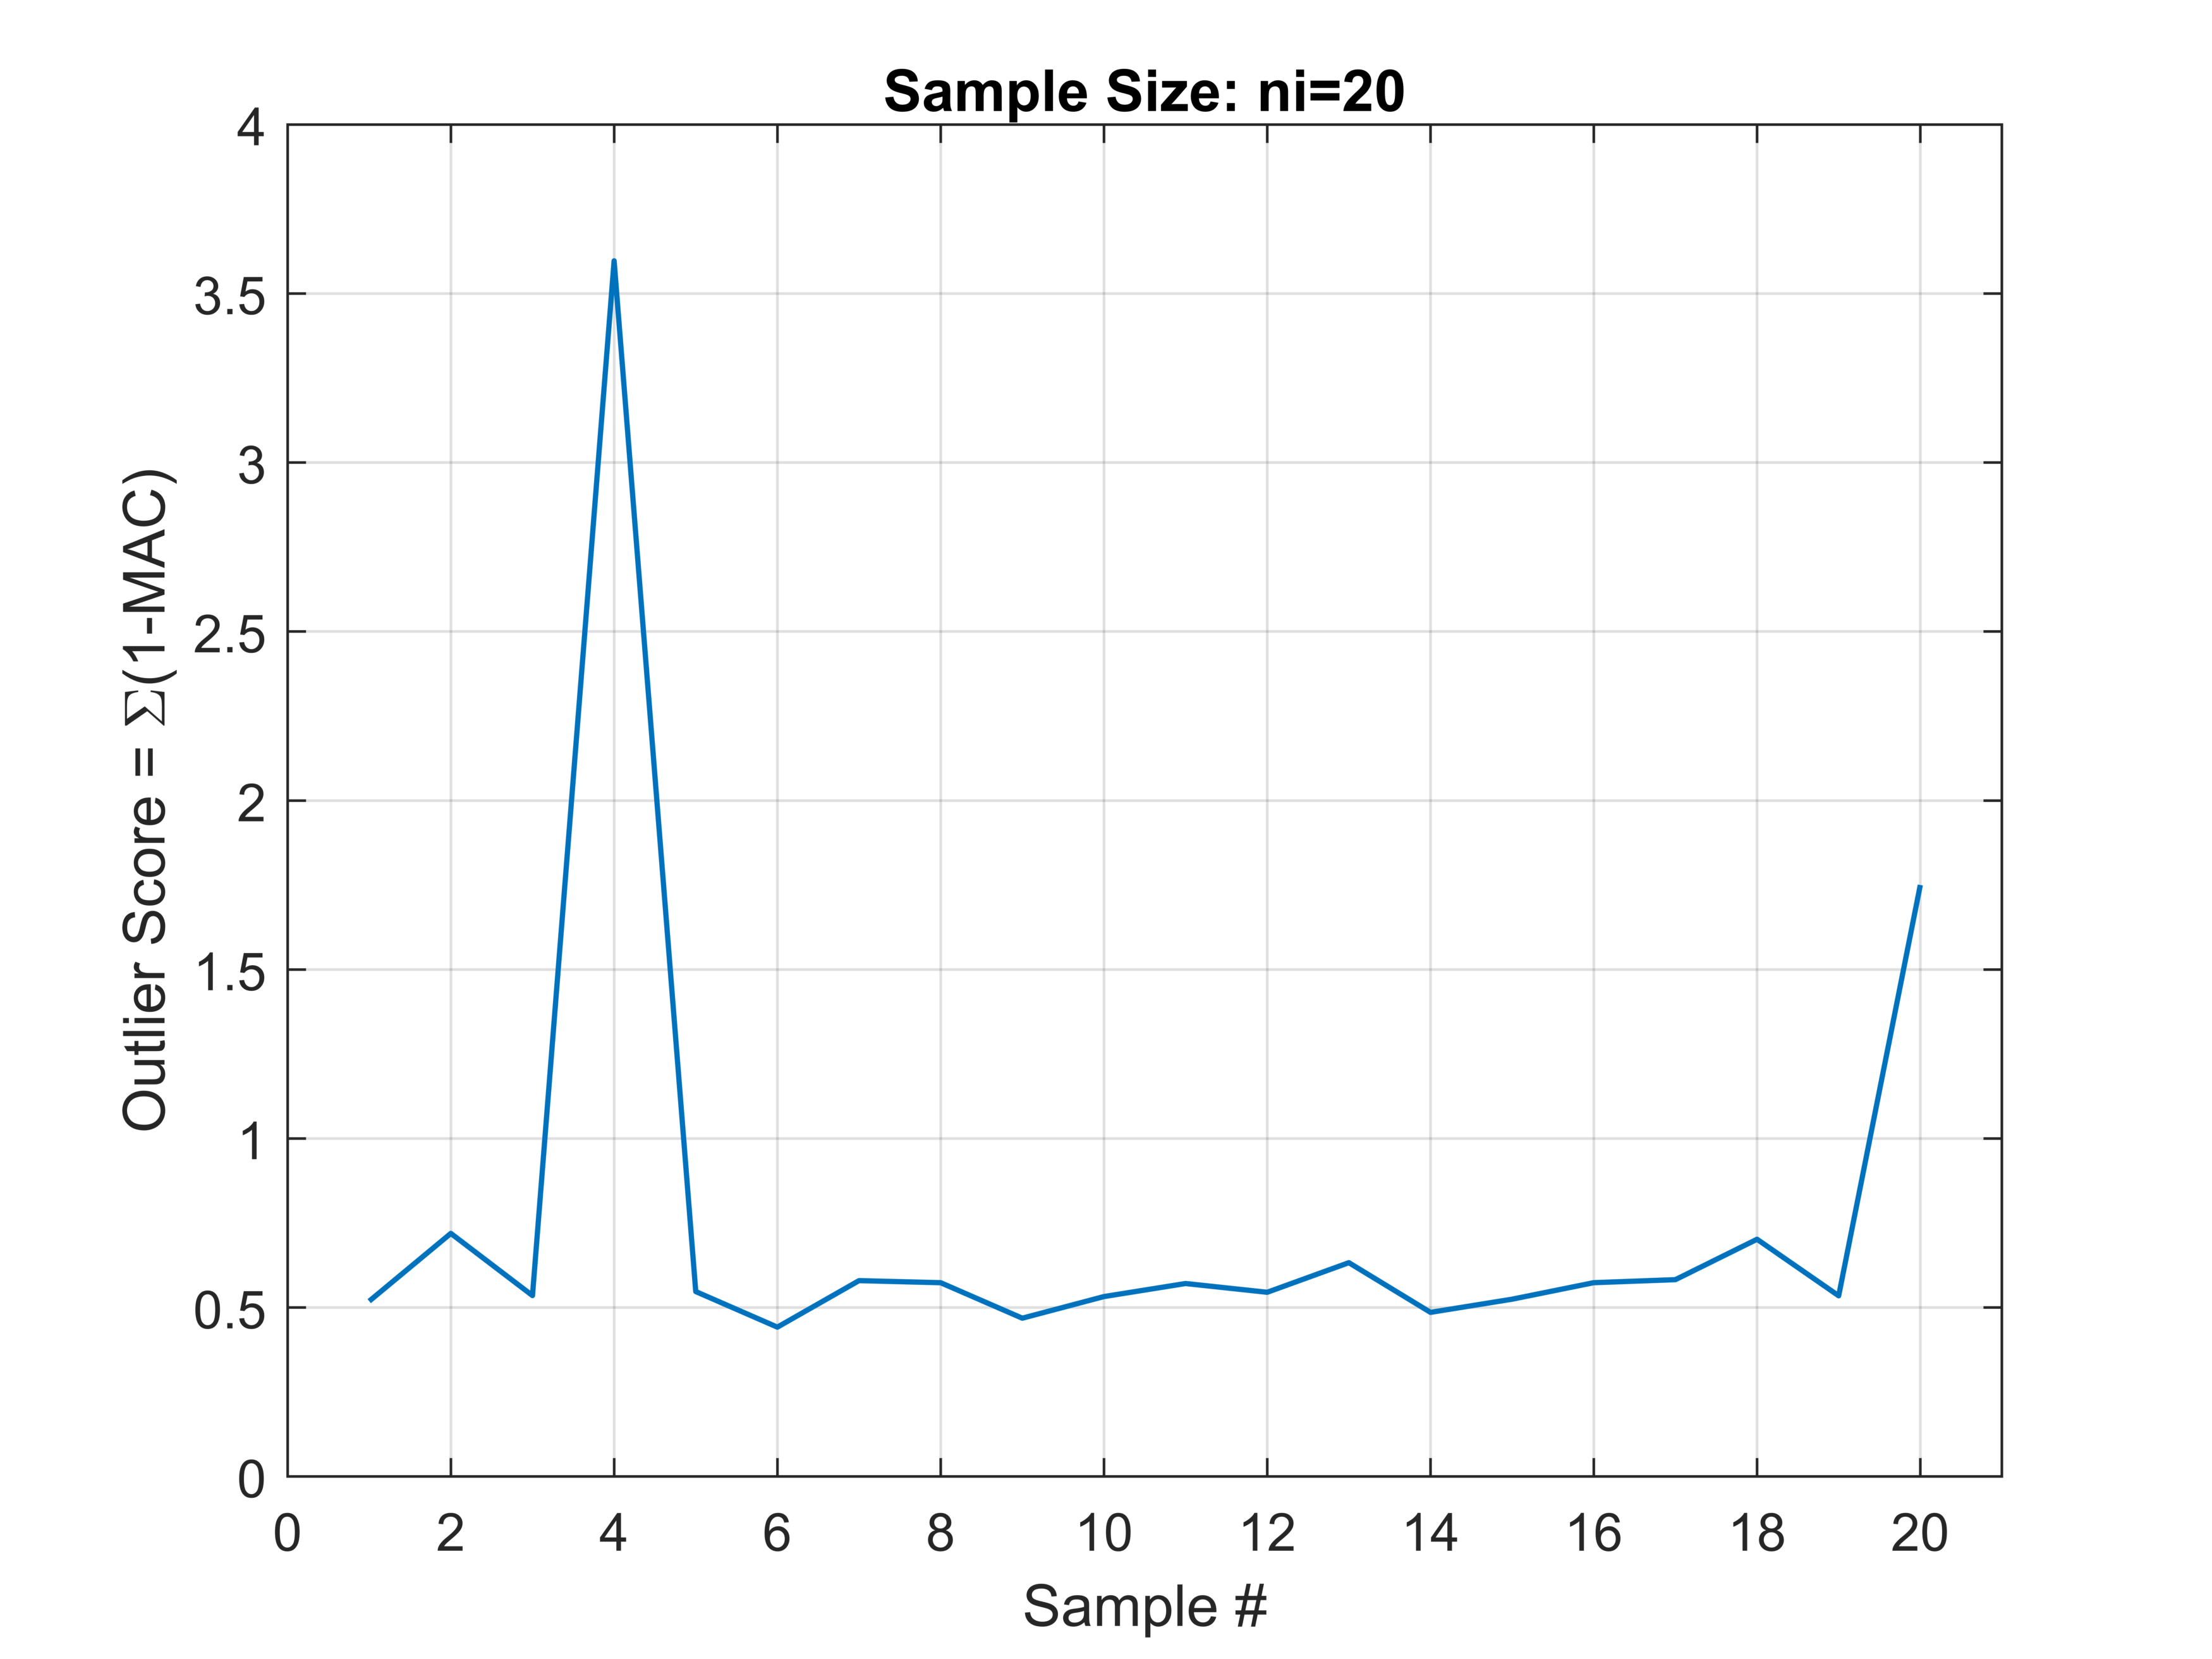
\includegraphics[width=0.48\textwidth]{MACscore_ni20}
\caption{MAC-based algorithm with a sample size of 20 (about 3 \% of the full data set).
Left: direct output of every sample; right: summed outputs are used as outlier score.
Among the 20 samples, \# 4 is truly an outlier and can be easily detected,
but \# 20 is actually an inlier and may be false positive if threshold are not chosen properly.
}
\label{fig:fig7}
\end{figure}

\begin{figure}[ht!]
\centering
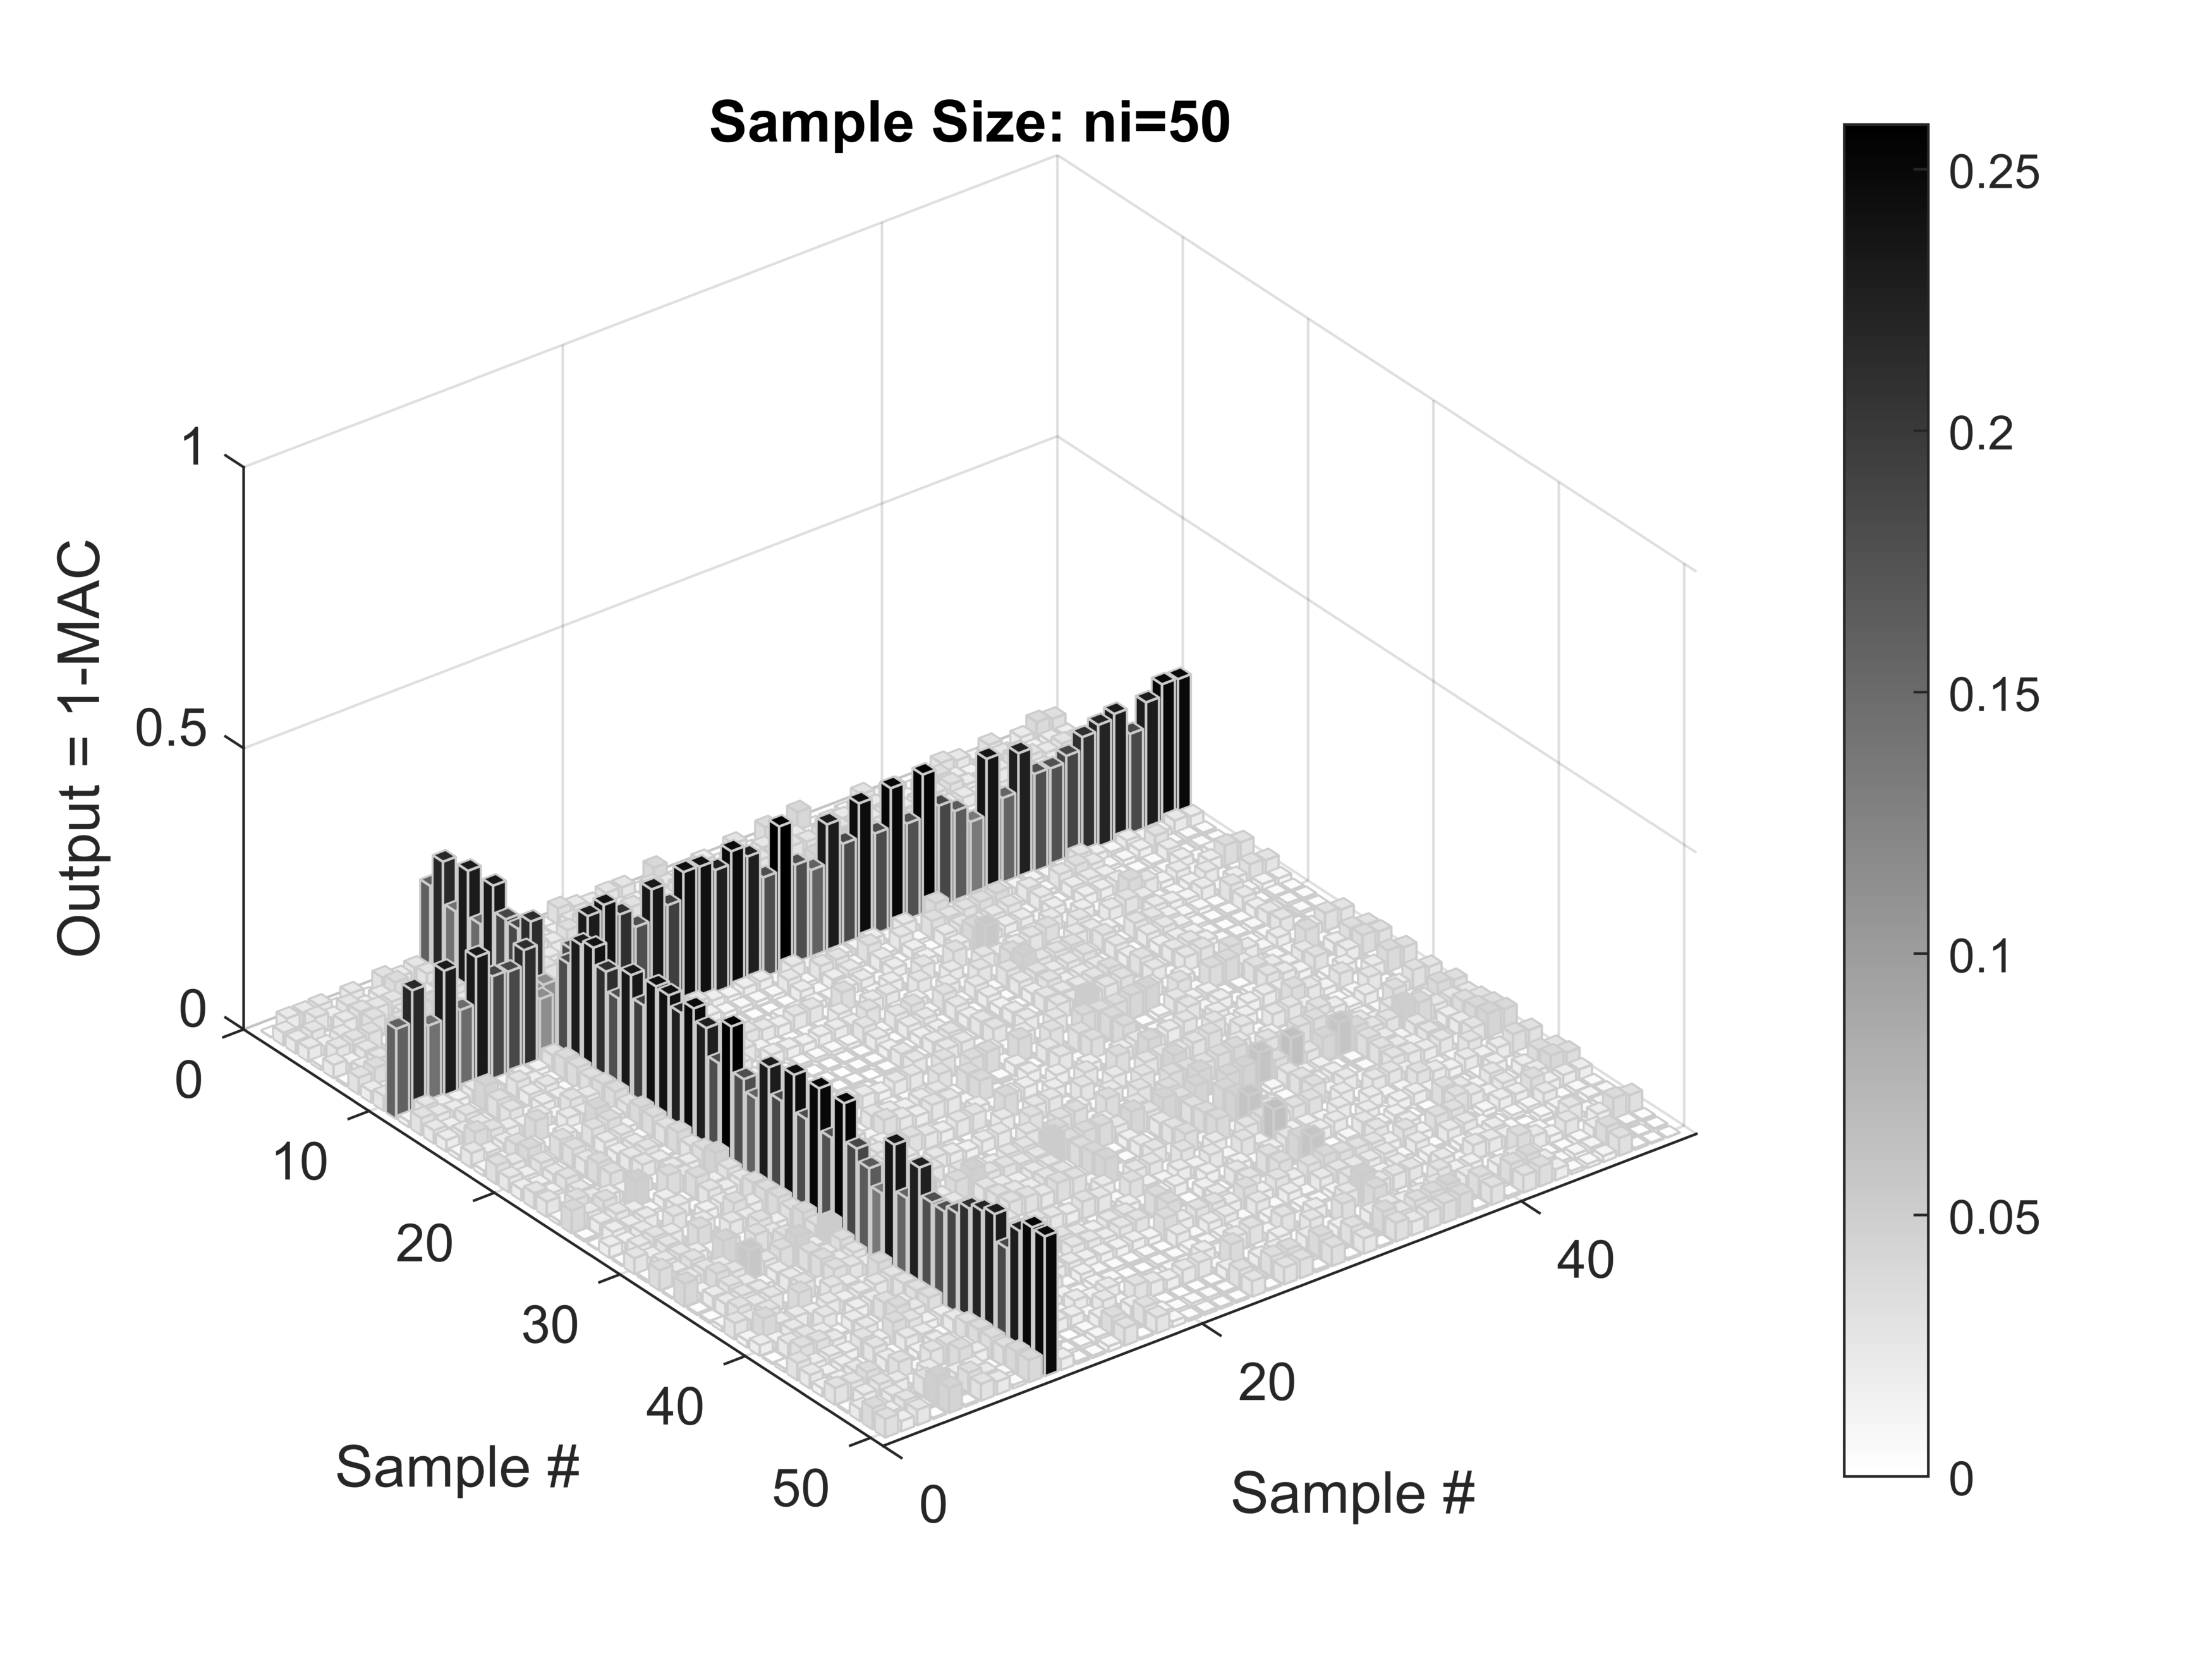
\includegraphics[width=0.48\textwidth]{MAC_ni50}
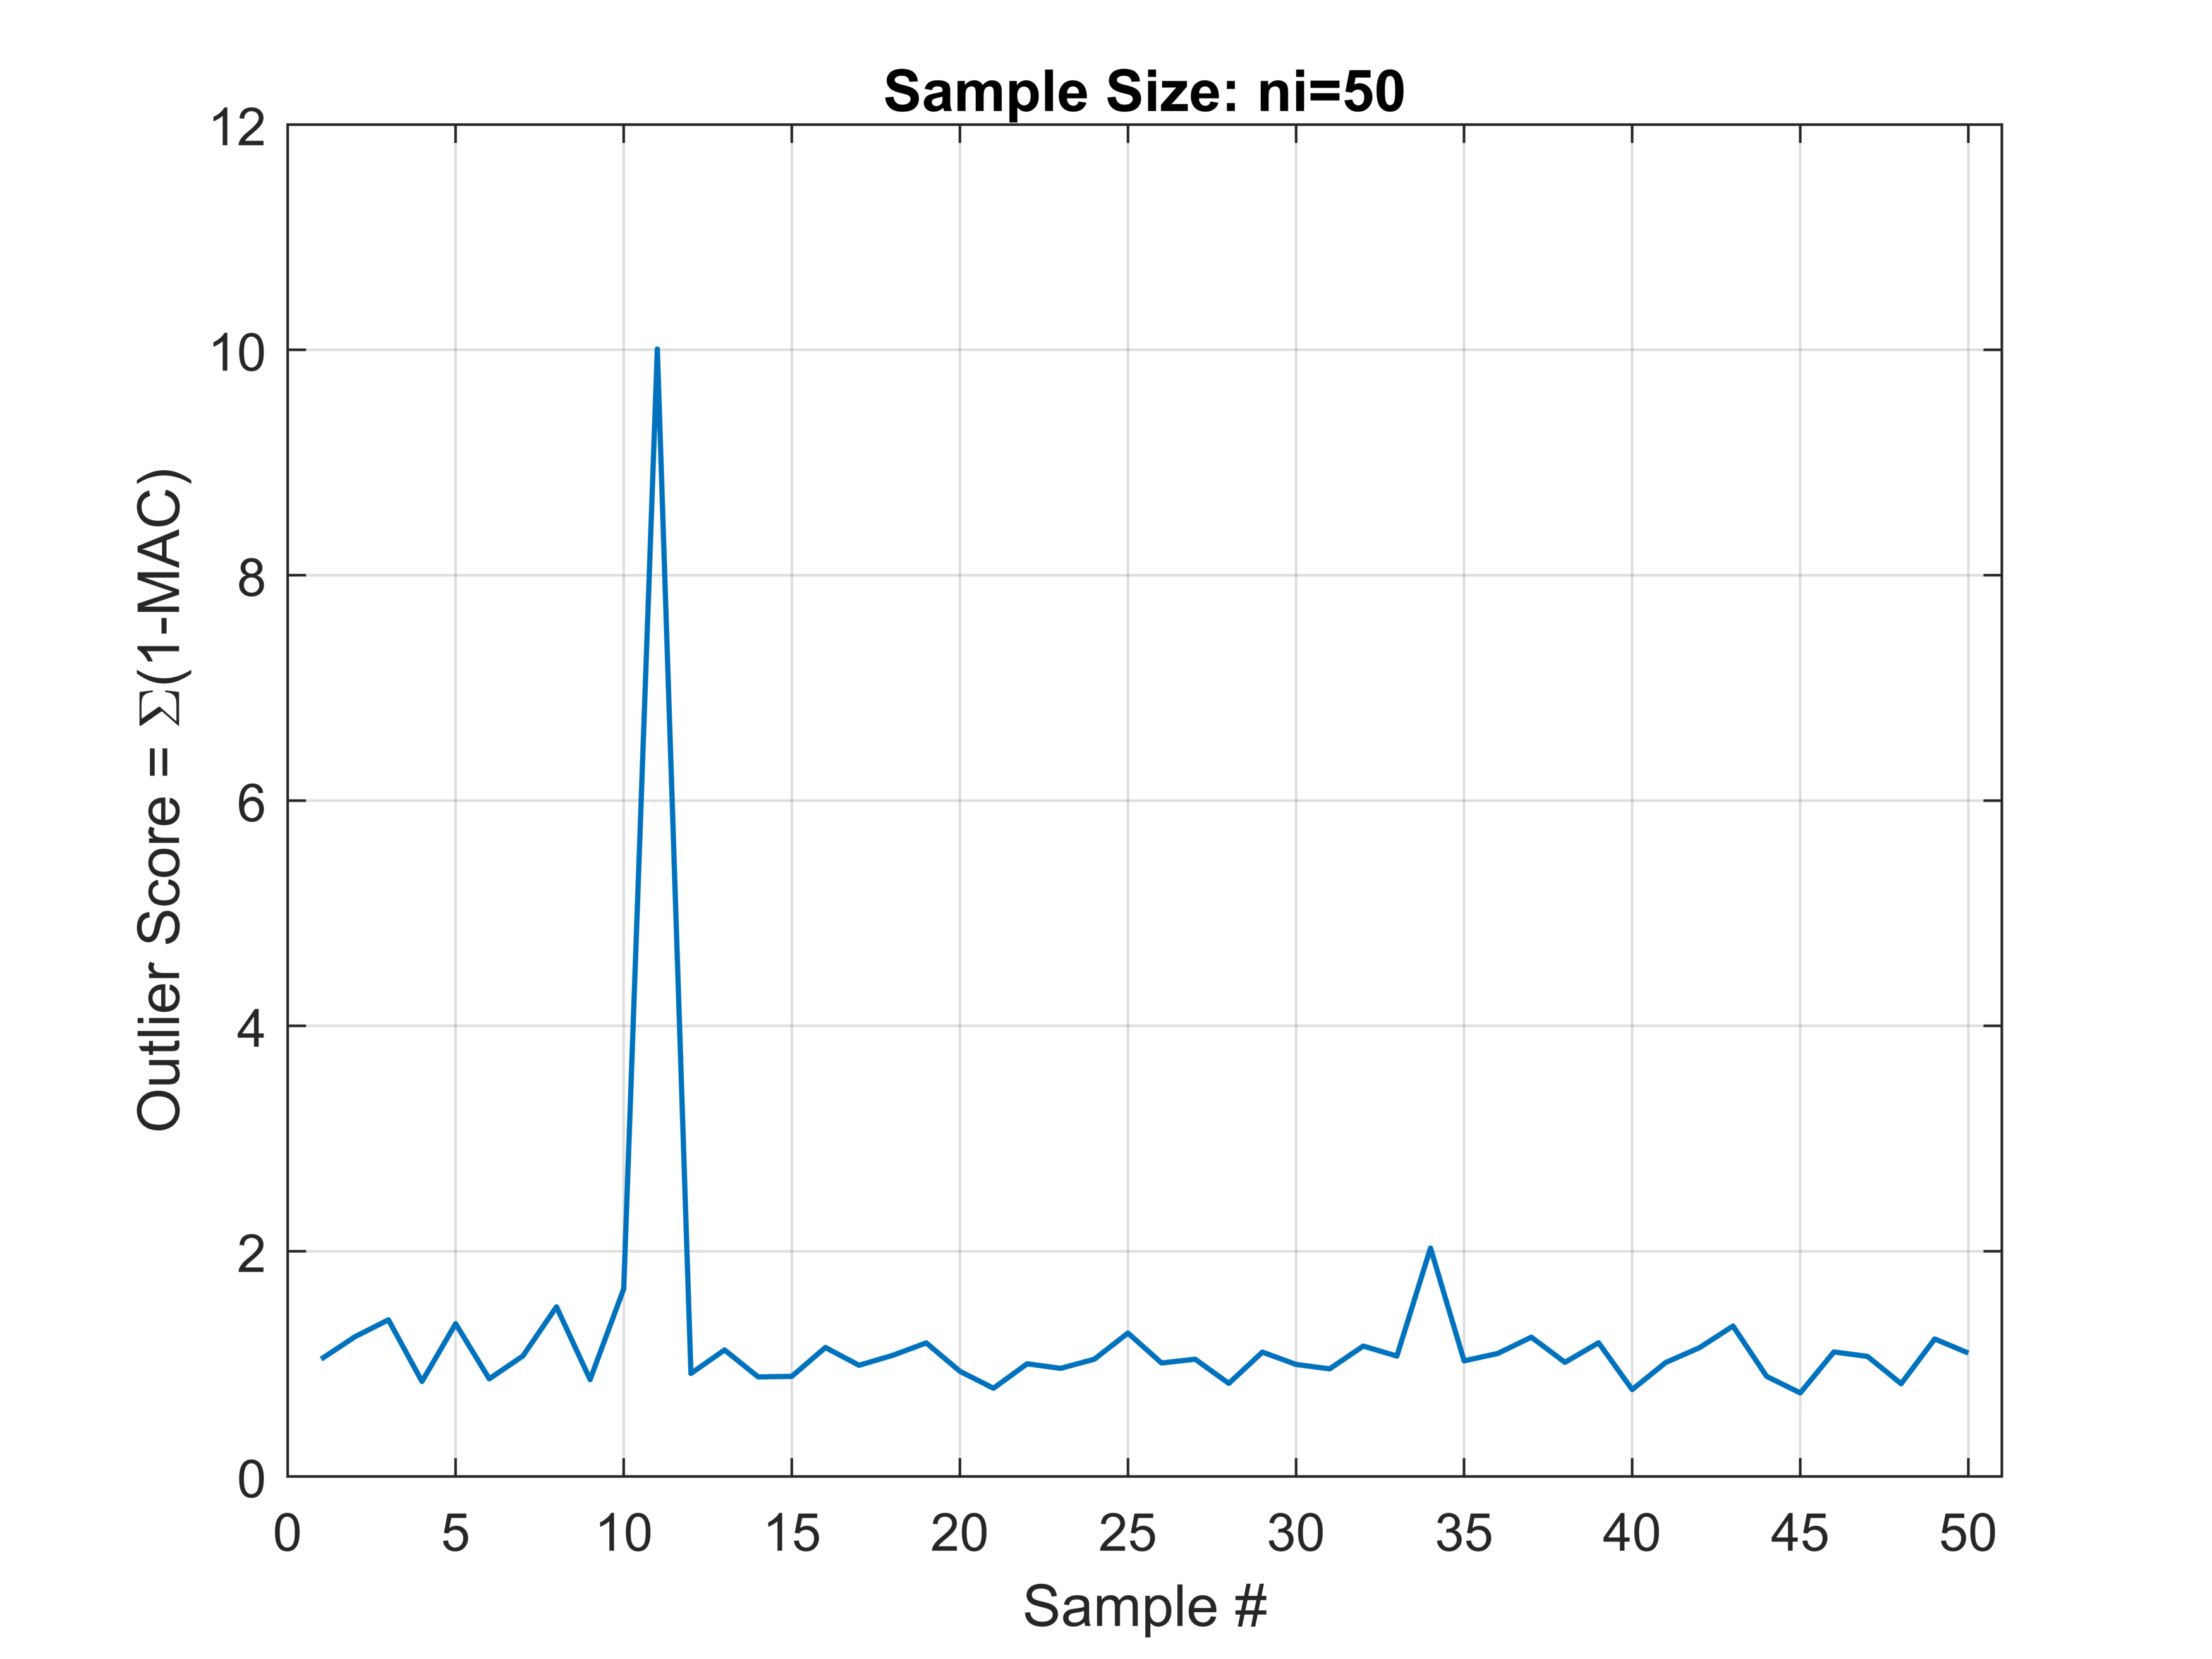
\includegraphics[width=0.48\textwidth]{MACscore_ni50}
\label{fig:fig8}
\caption{MAC-based algorithm with a sample size of 50 (about 8 \% of the full data set).
Left: direct output of every sample; right: summed outputs are used as outlier score.
Among the 50 samples, \# 11 is truly an outlier and can be easily detected.}
\end{figure}


\begin{figure}[ht!]
\centering
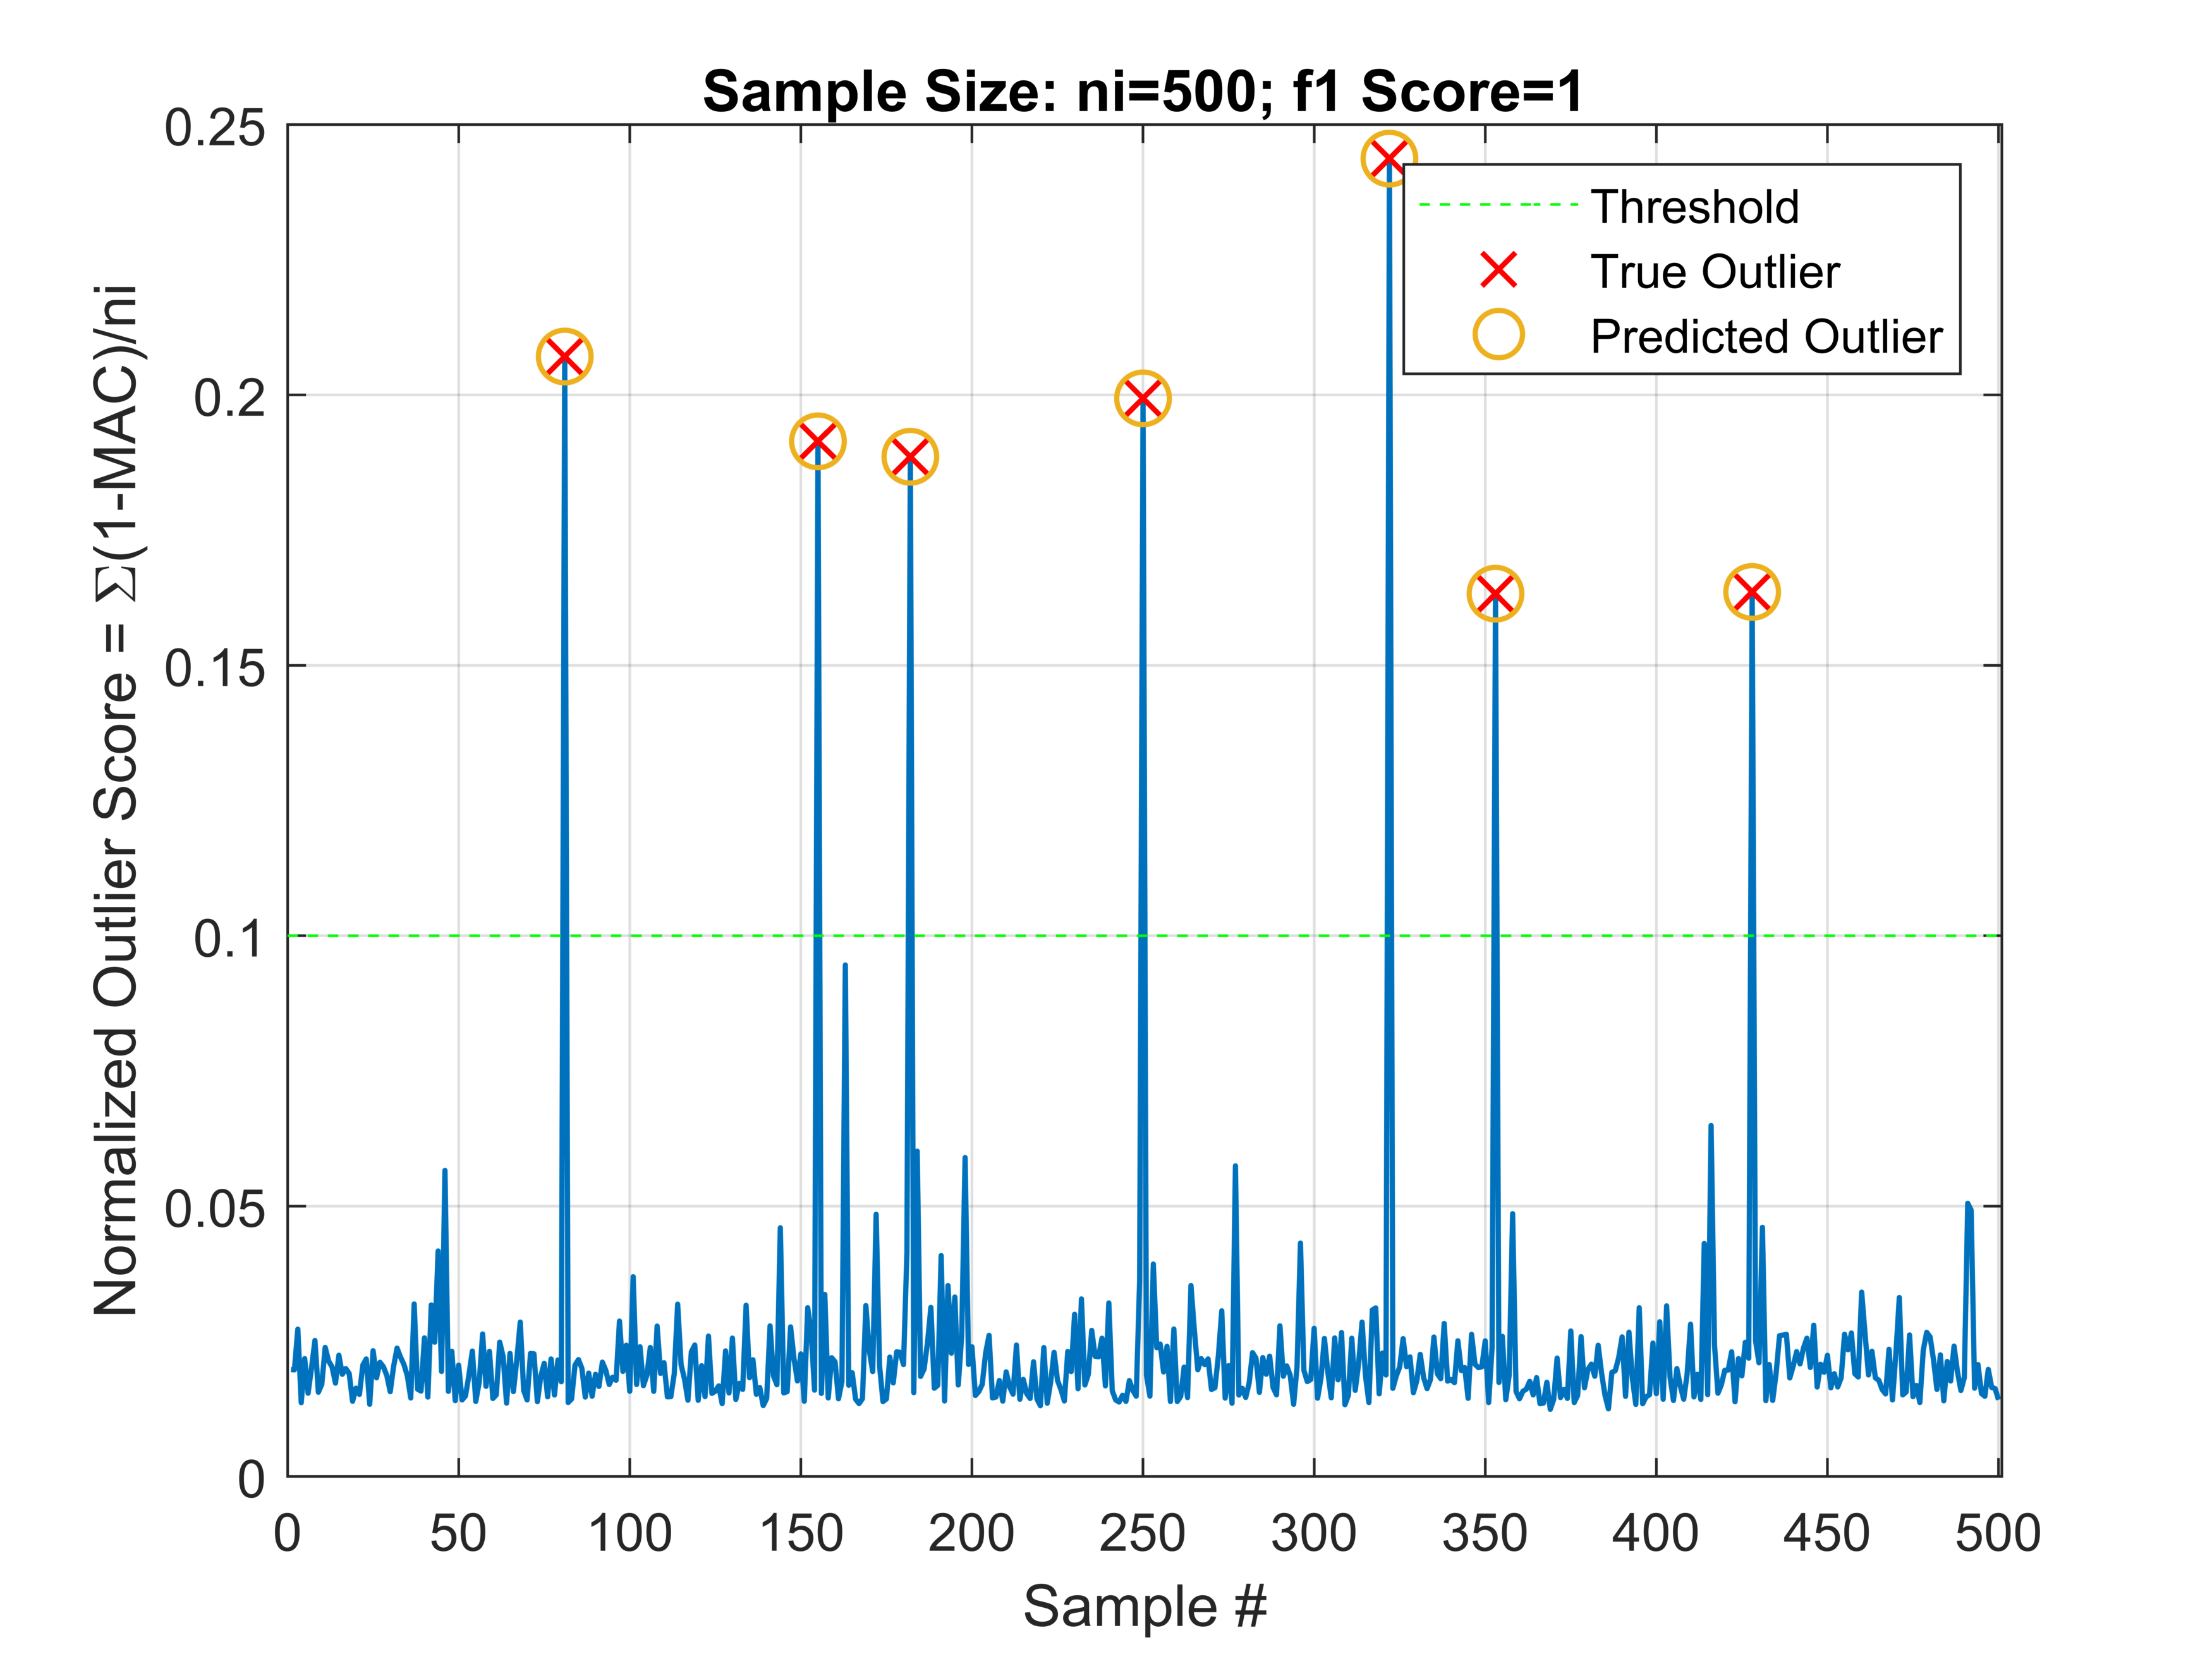
\includegraphics[width=0.85\textwidth]{f1score_ni500}
\caption{MAC-basd algorithm with normalized outlier score on 500 samples.}
\label{fig:fig9}
\end{figure}

\begin{figure}[ht!]
\centering
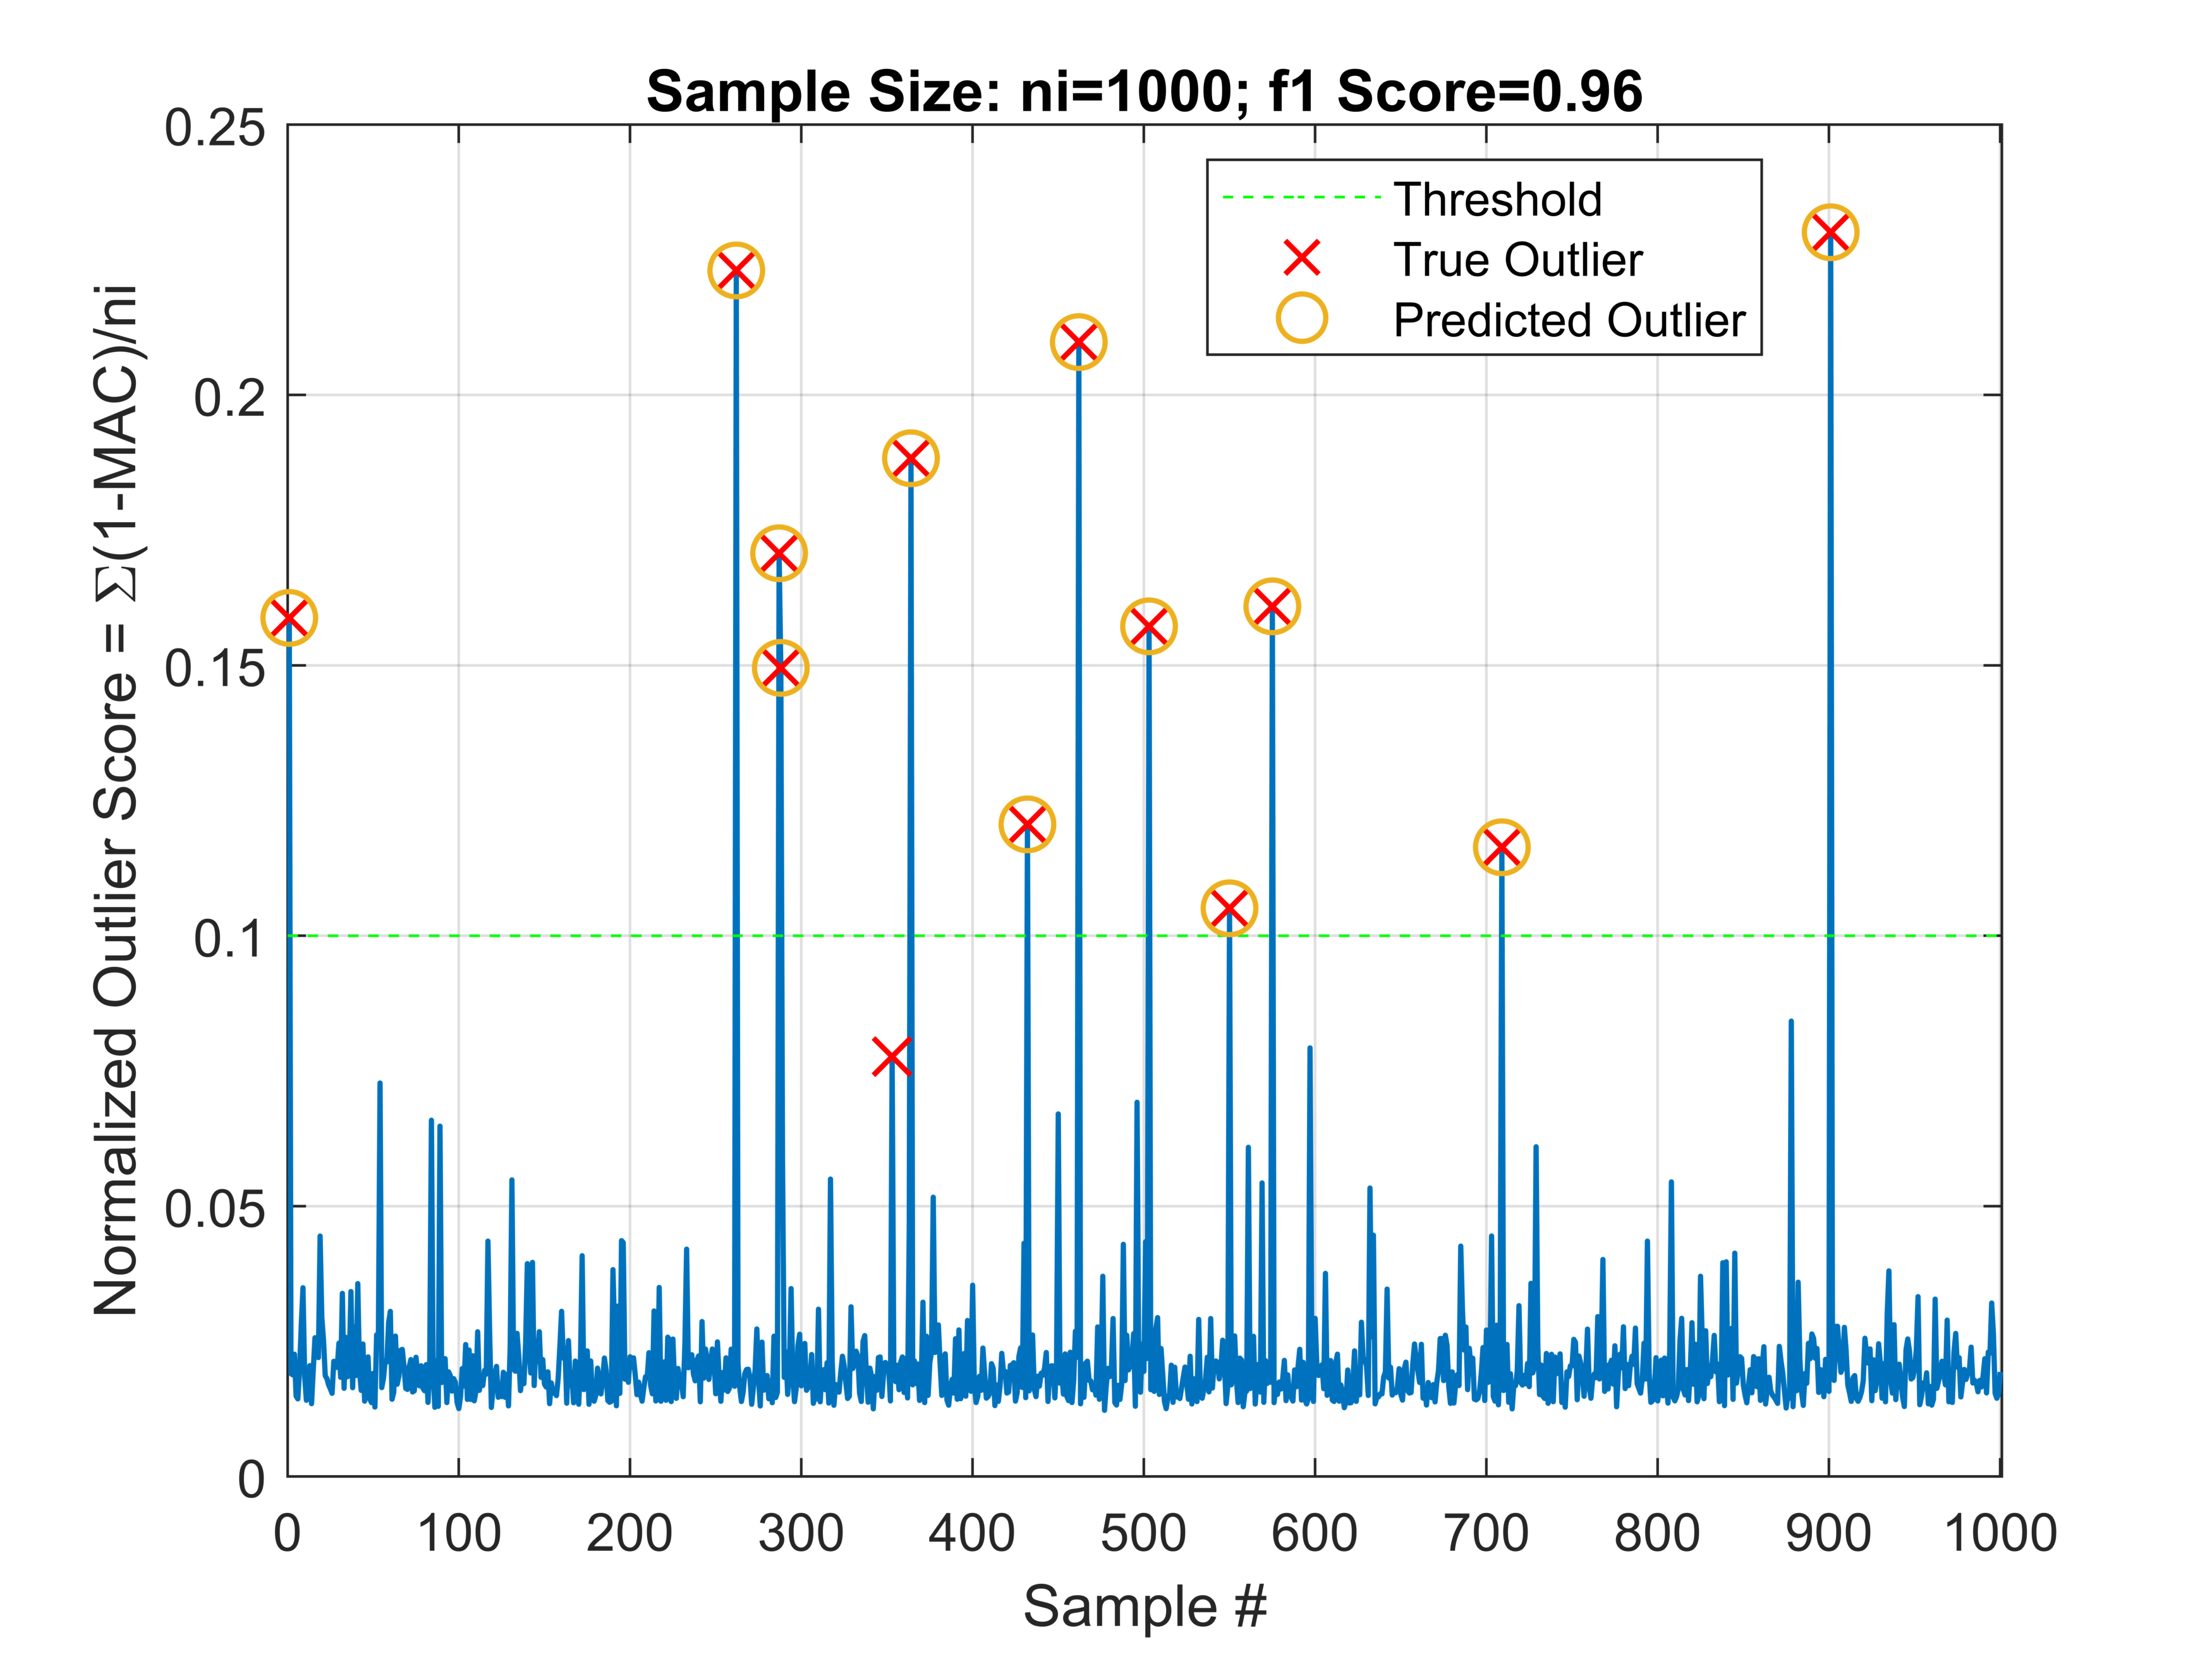
\includegraphics[width=0.85\textwidth]{f1score_ni1000}
\caption{MAC-basd algorithm with normalized outlier score on 1000 samples.}
\label{fig:fig10}
\end{figure}

\begin{figure}[ht!]
\centering
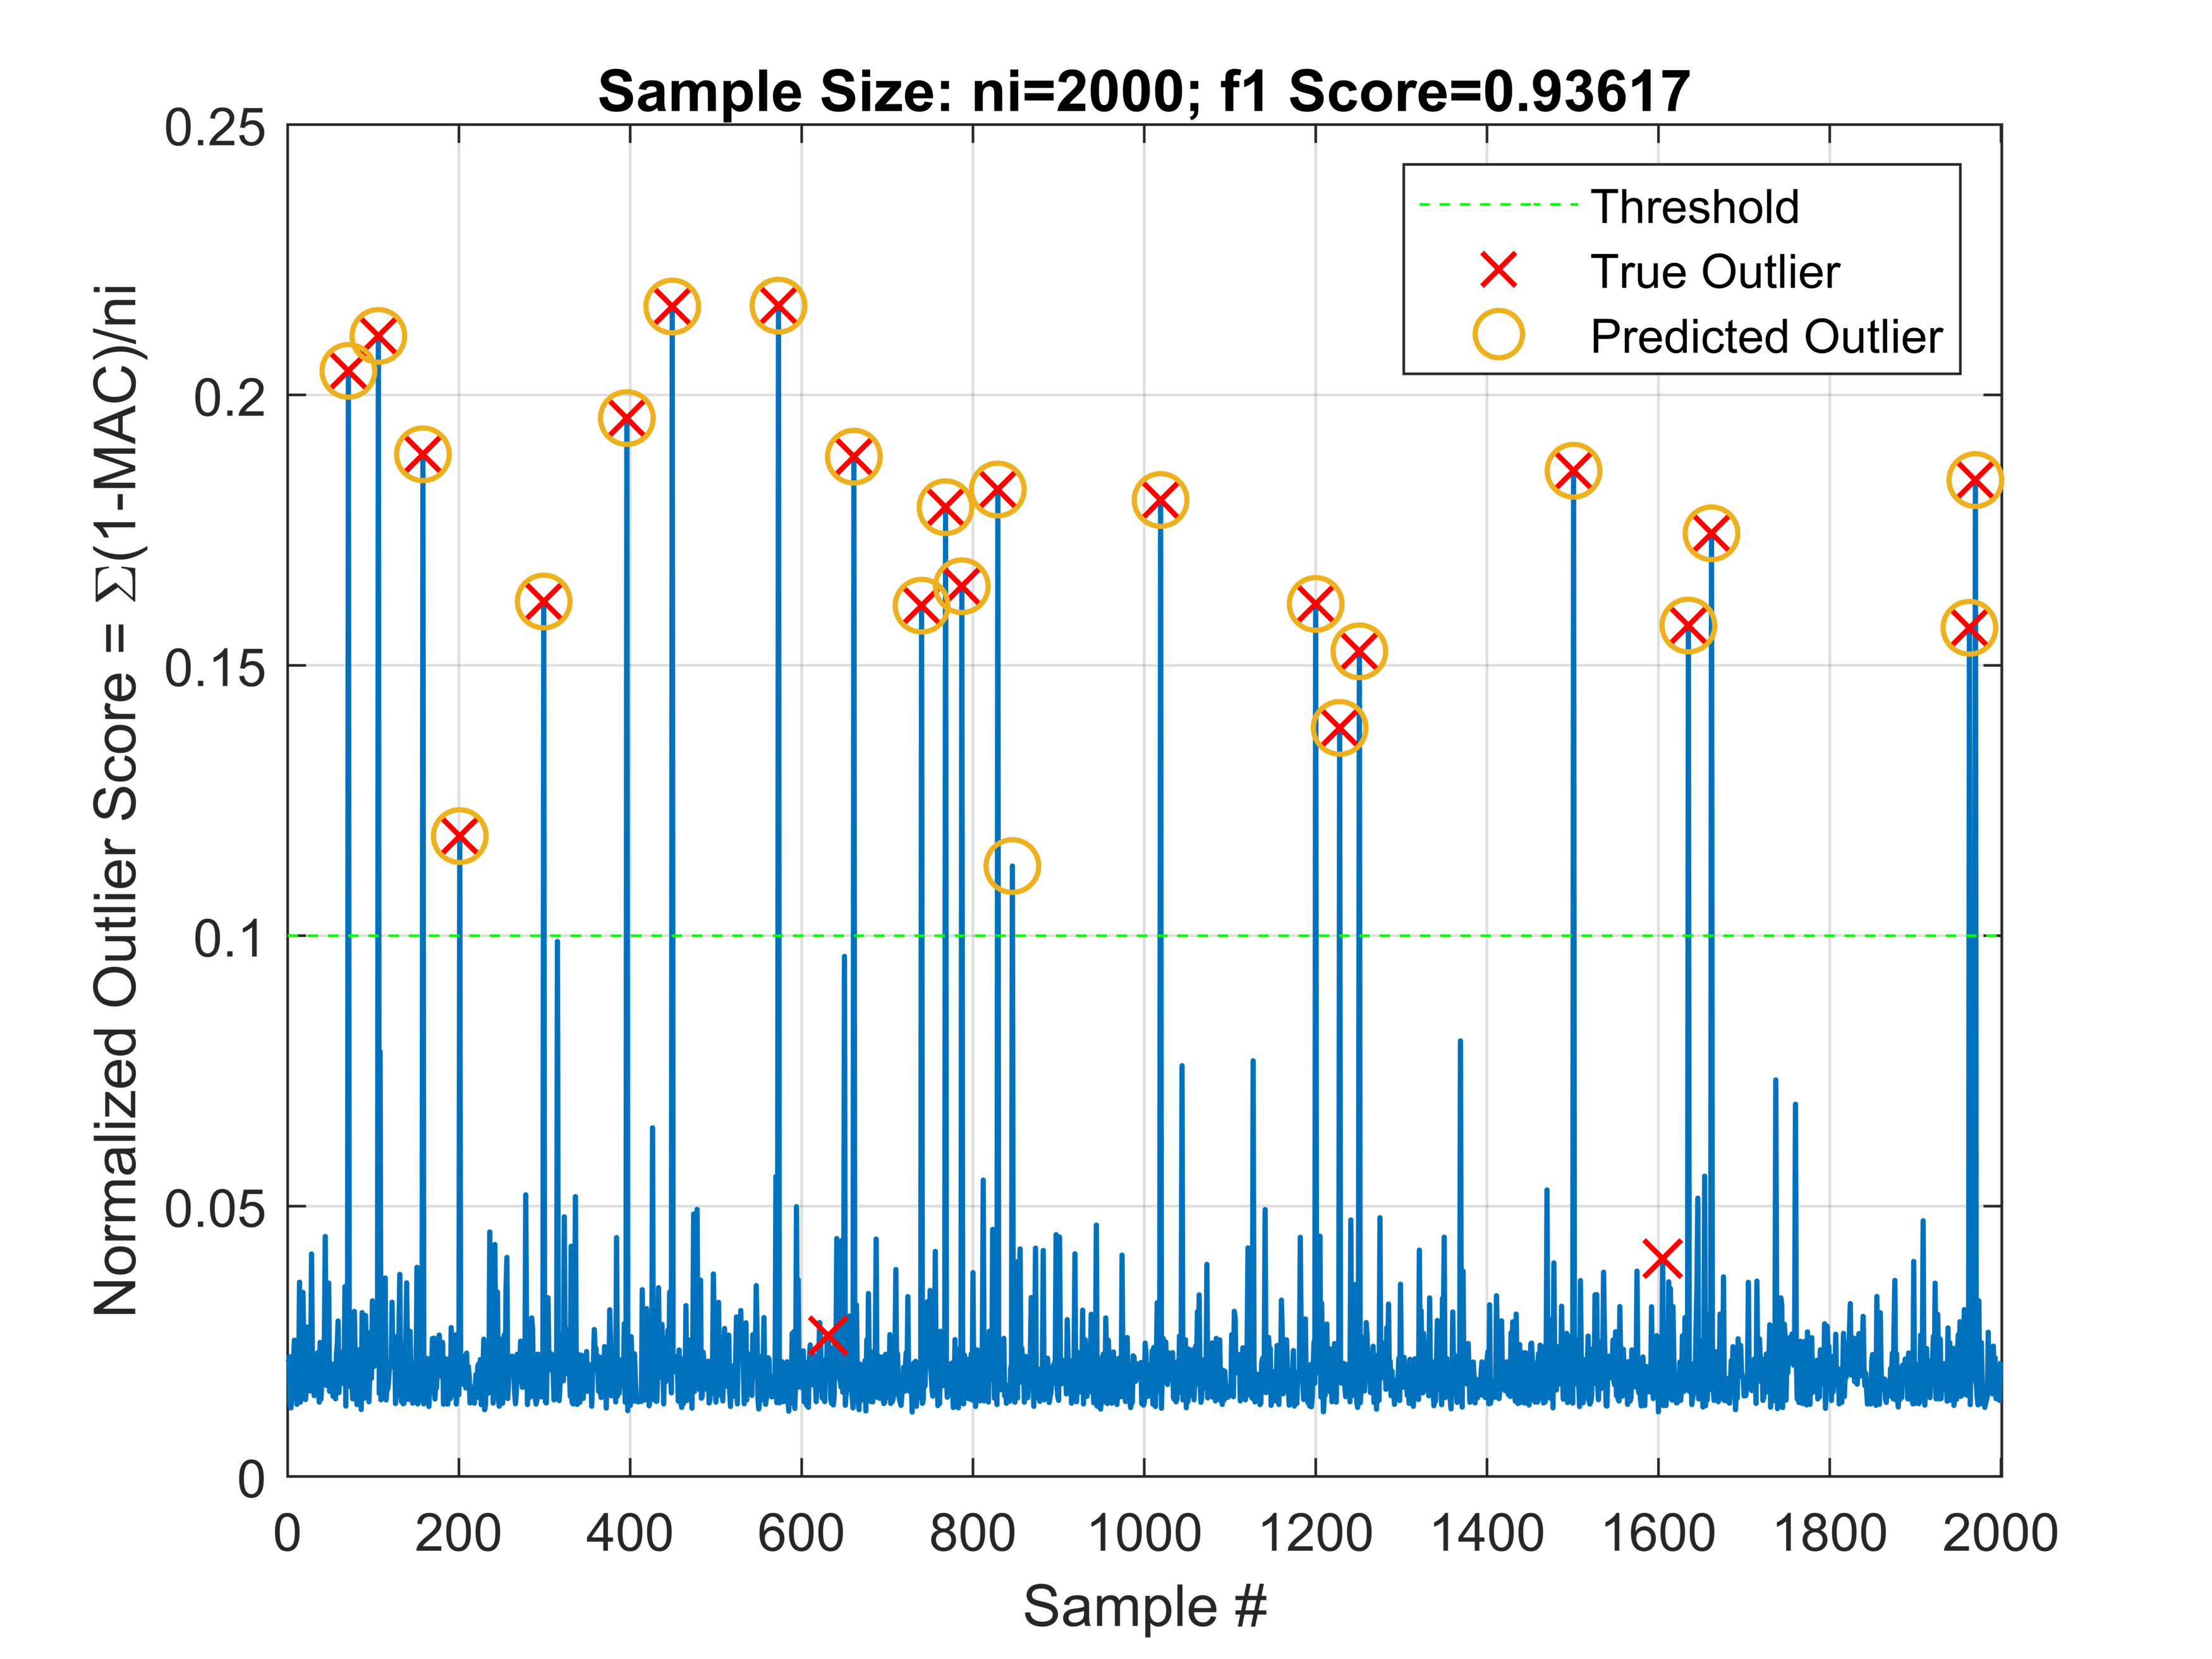
\includegraphics[width=0.85\textwidth]{f1score_ni2000}
\caption{MAC-basd algorithm with normalized outlier score on 2000 samples.}
\label{fig:fig11}
\end{figure}

\begin{figure}[ht!]
\centering
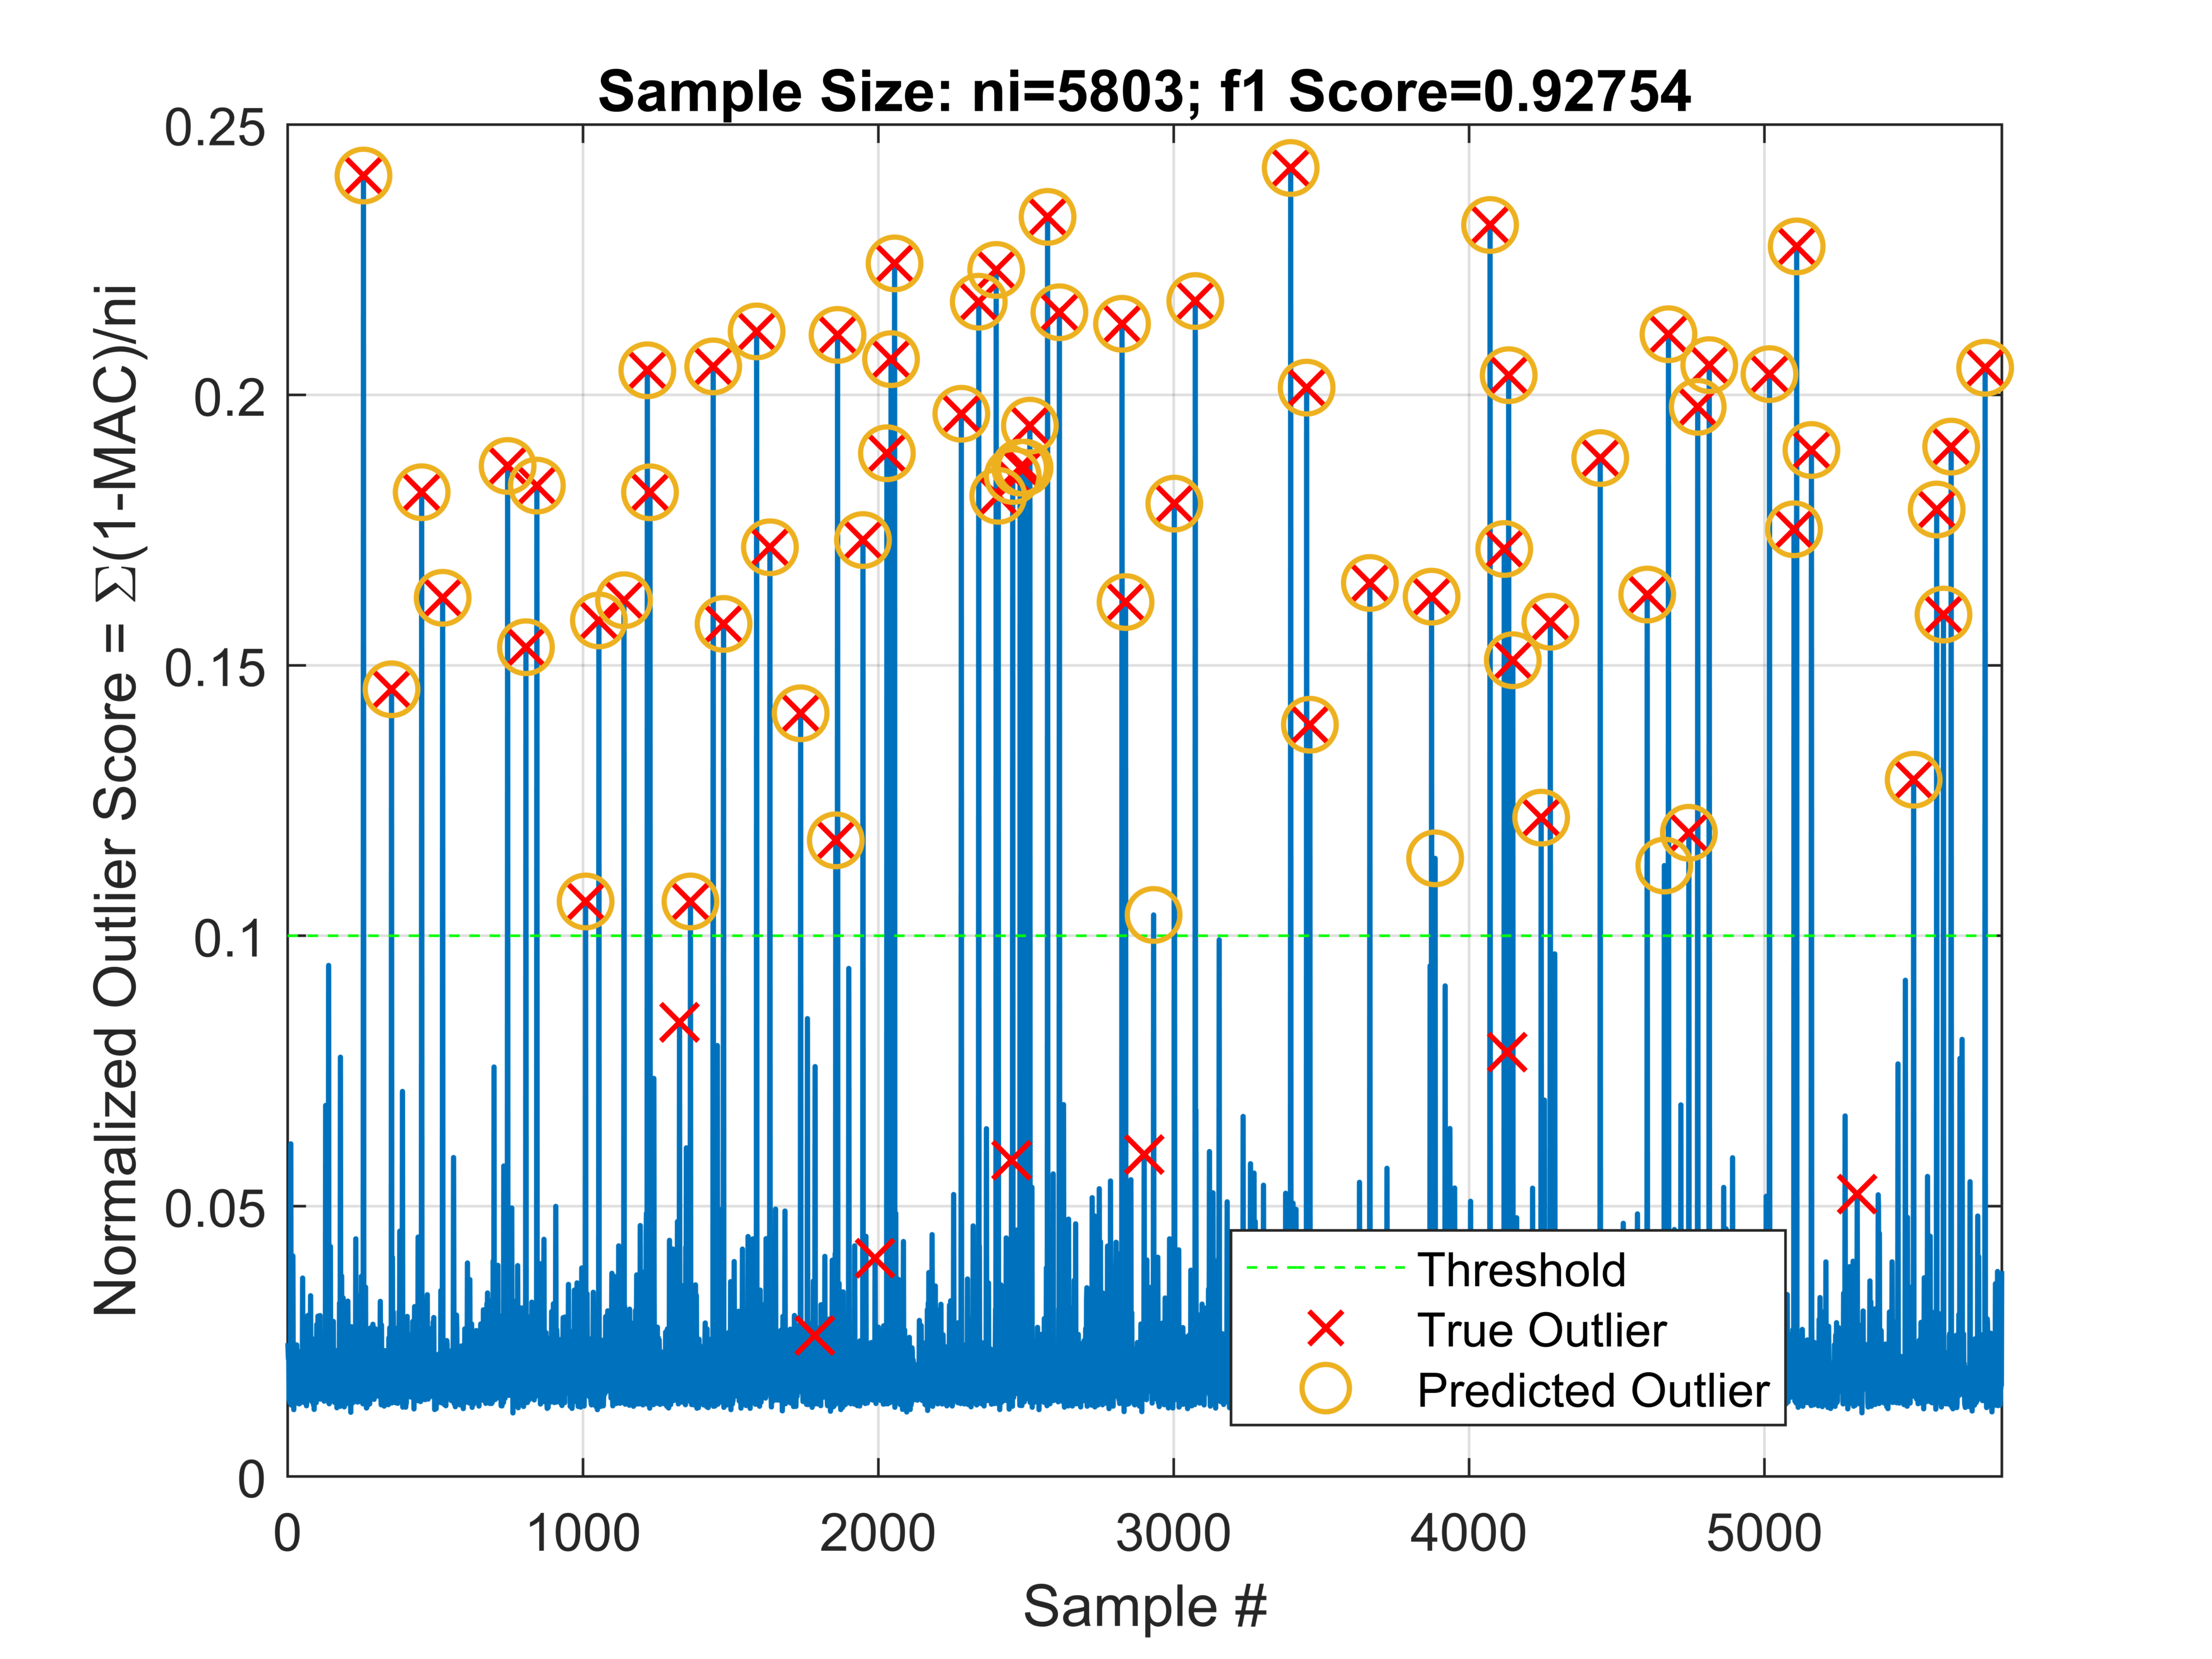
\includegraphics[width=0.85\textwidth]{f1score_ni5803}
\caption{MAC-basd algorithm with normalized outlier score on the full data set.}
\label{fig:fig12}
\end{figure}

Different than the KNN algorithm, my MAC-based algorithm uses all other samples 
to calculate the outlier score, and therefore I do not have to investigate an extra
hyper-parameter $k$. My algorithm requires at least three samples to work, and I have tested how
the algorithm performs in very few samples as well, as shown in Figure 13. 
However, due to the limited time, I did not ingestive the performance variance of my algorithm using 
multiple trails and only one insistent of each sample size is reported here.

\begin{figure}[ht!]
\centering
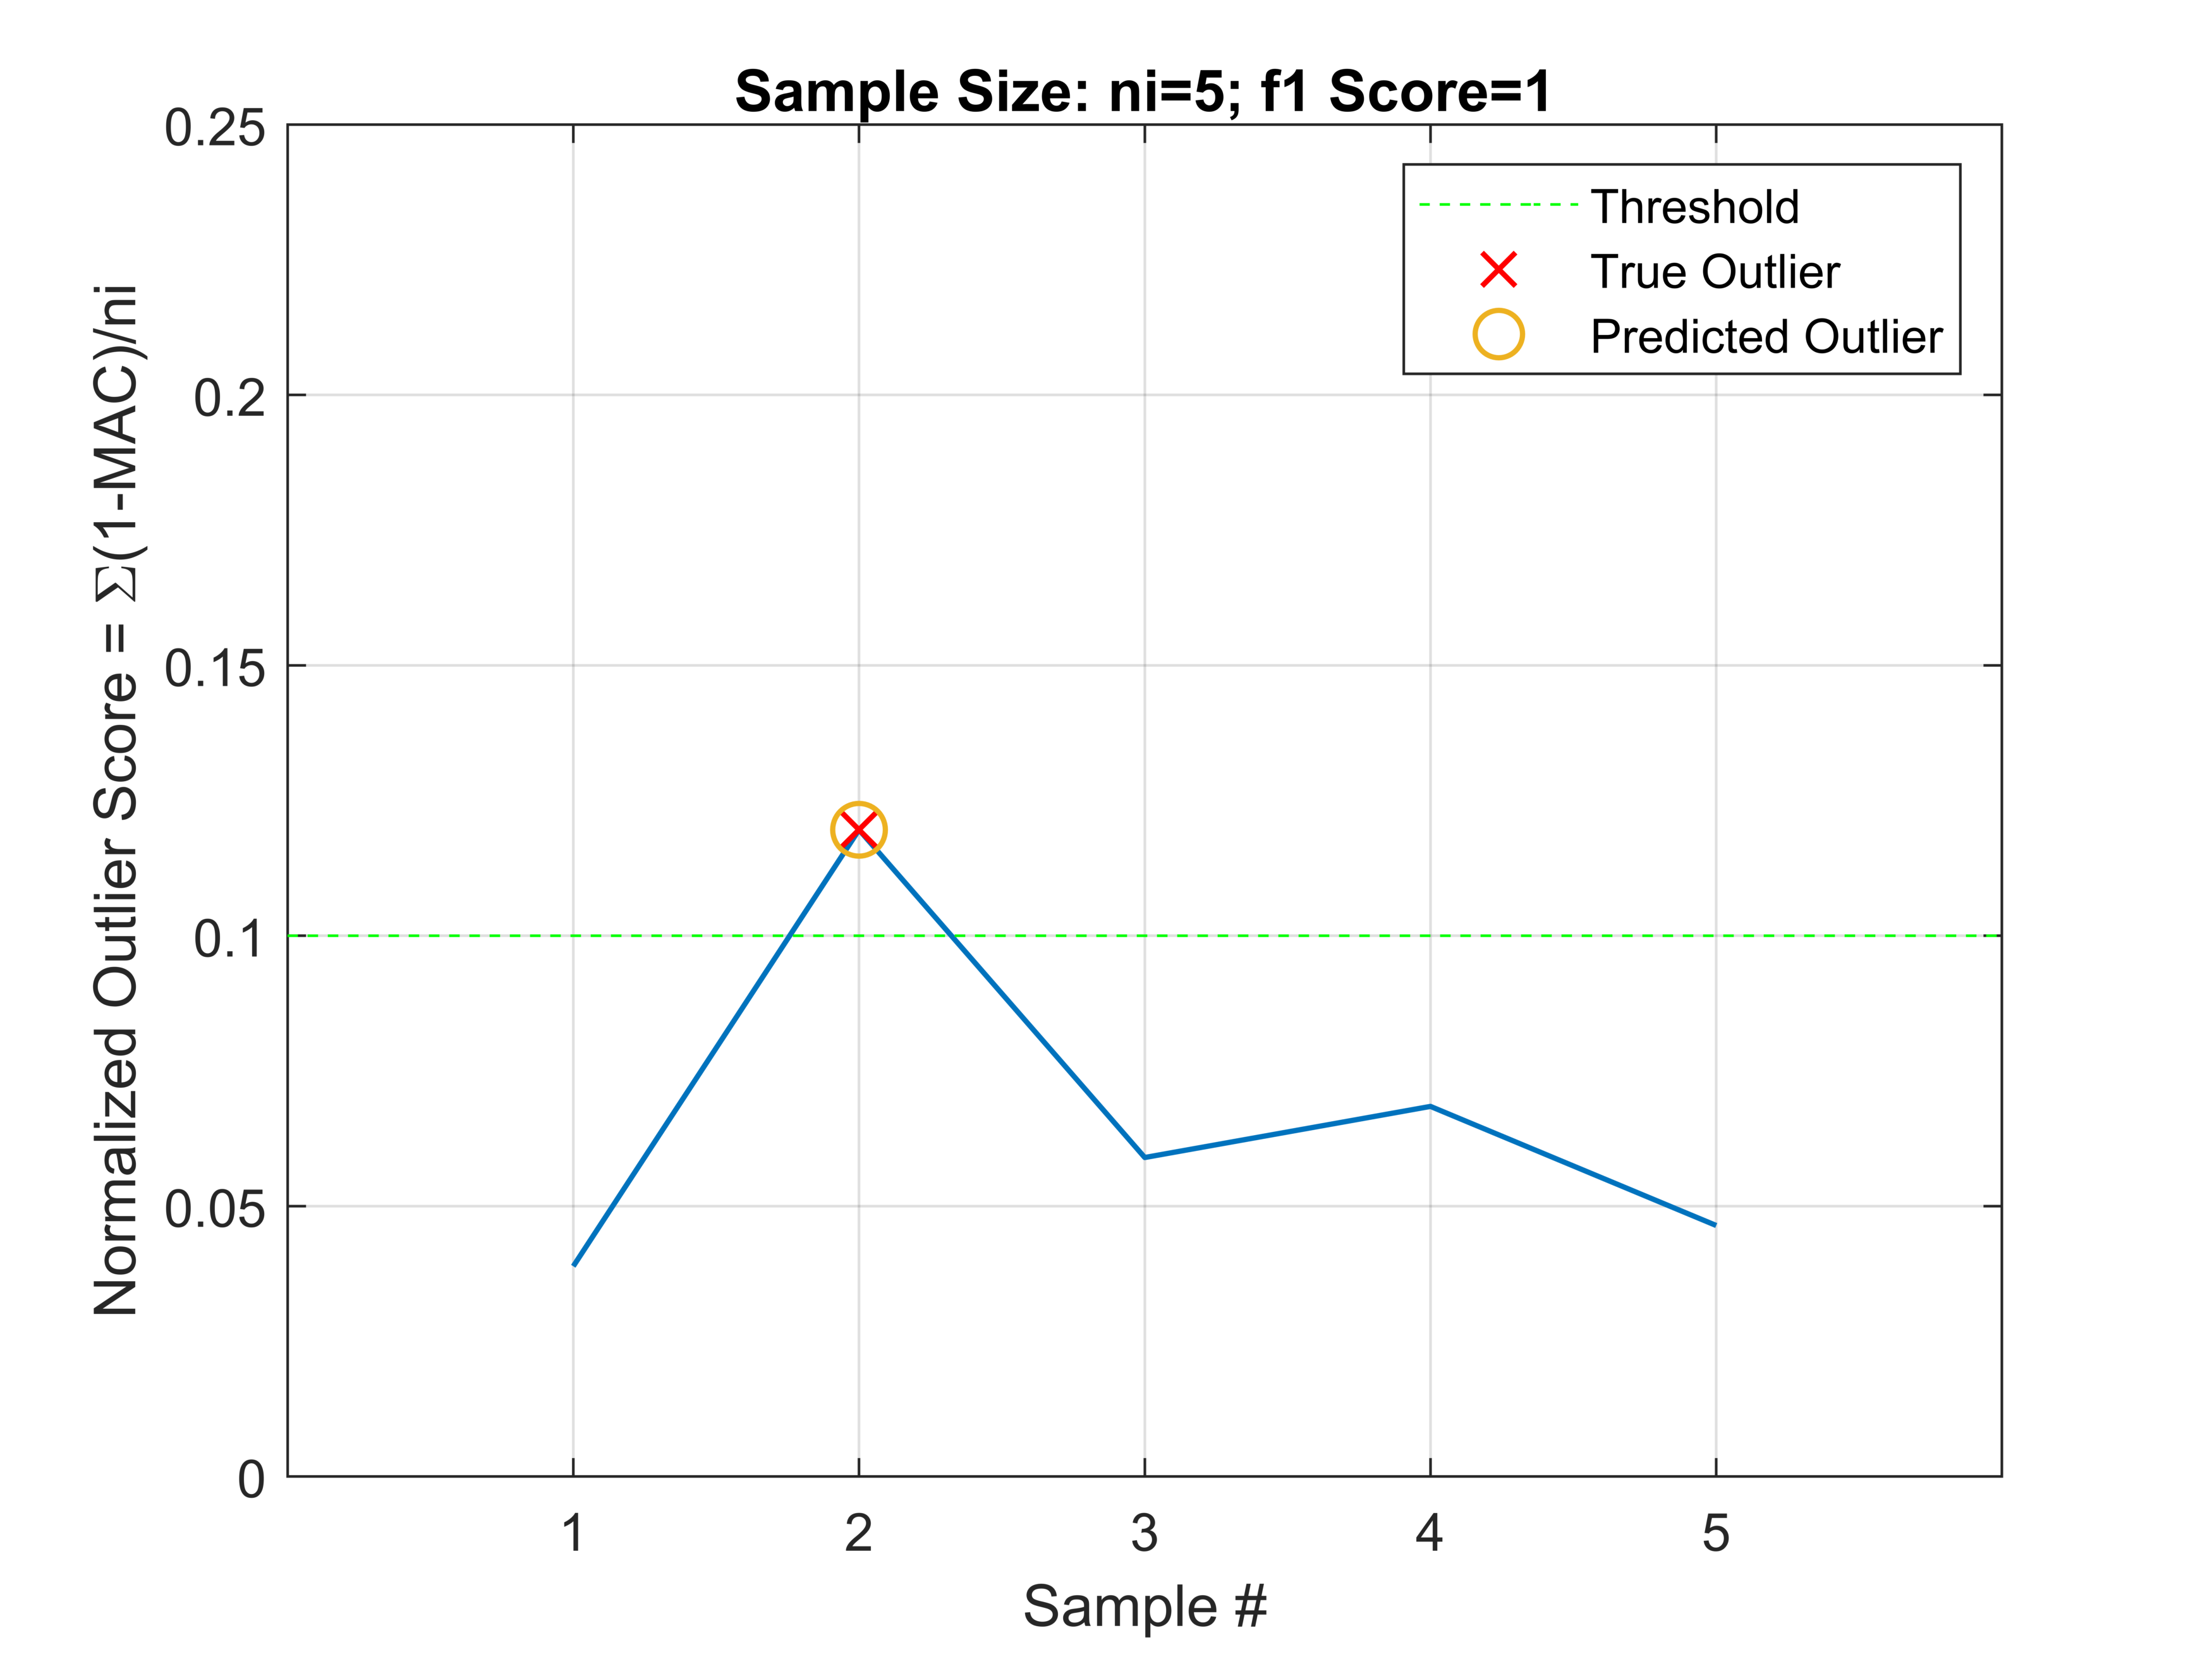
\includegraphics[width=0.48\textwidth]{f1score_ni5}
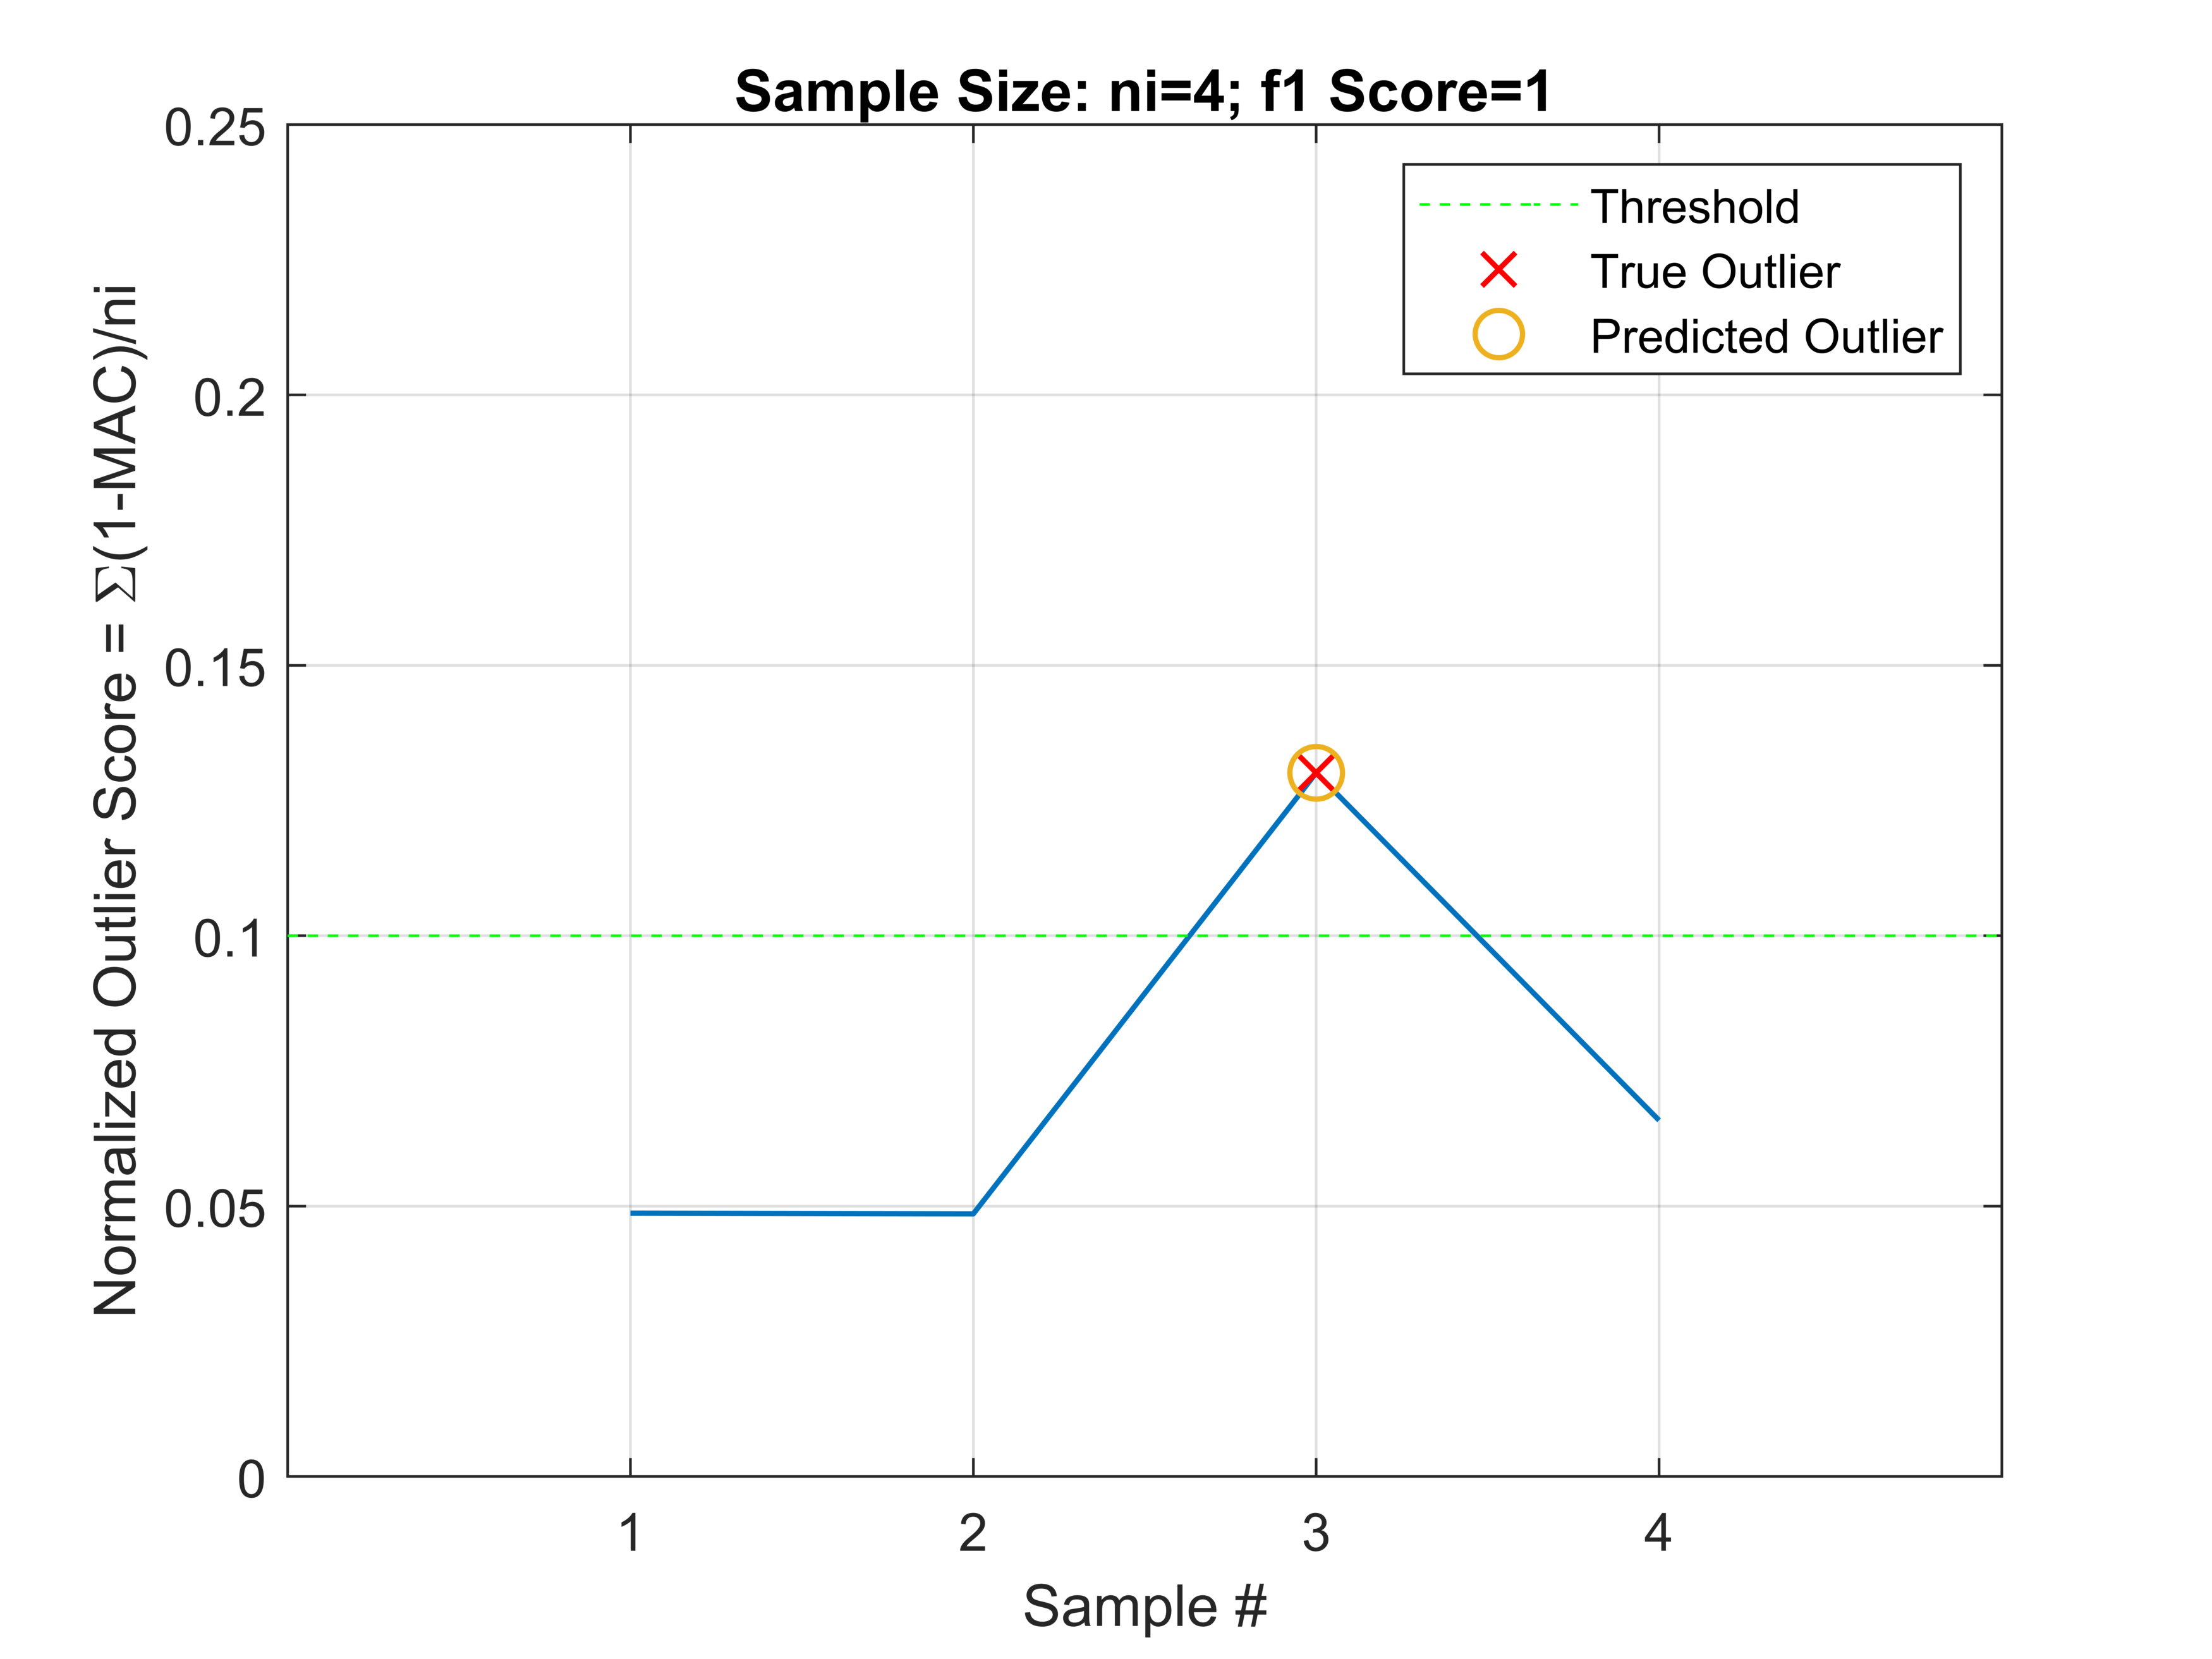
\includegraphics[width=0.48\textwidth]{f1score_ni4}
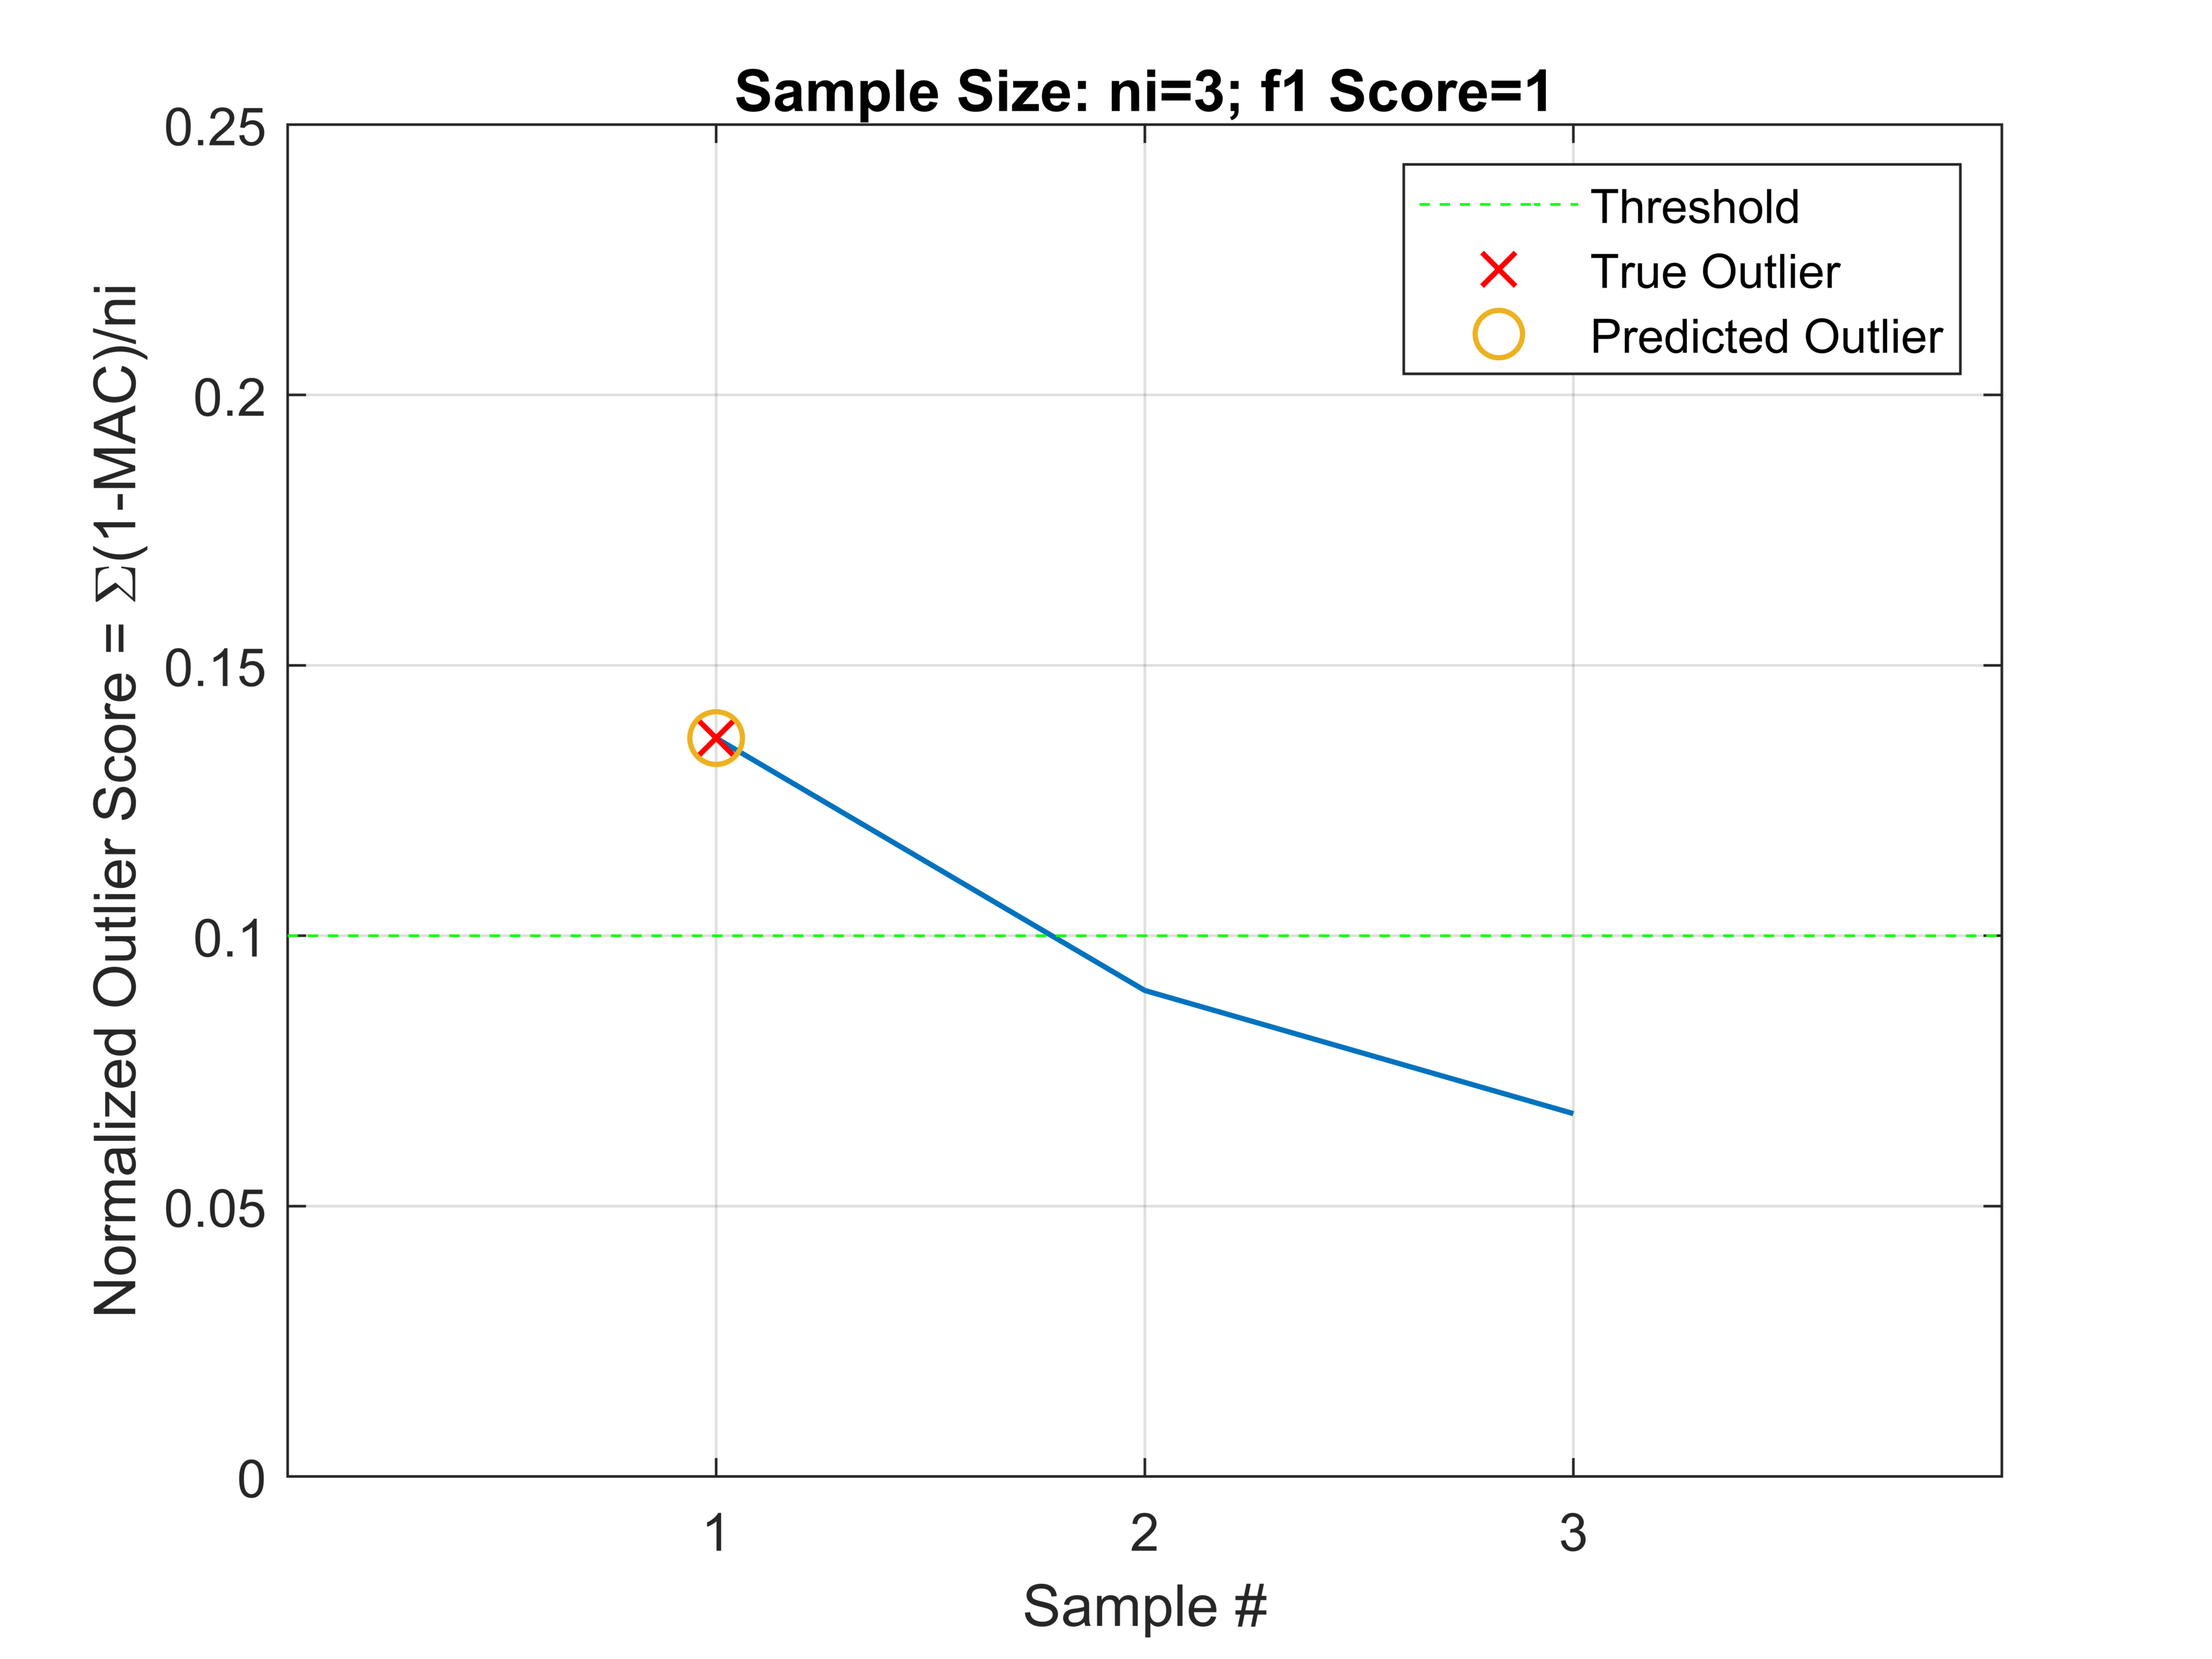
\includegraphics[width=0.48\textwidth]{f1score_ni3}
\caption{MAC-basd algorithm with normalized outlier score on very small sample sizes.}
\label{fig:fig13}
\end{figure}

\pagebreak
\section{Epilogue}

This coding exercise for oulier detection is surprisingly interesting, and I enjoy greatly 
during the process of discovery. Despite my limited experience in machine learning, I mobilized my 
knowledge and tools in my exiting domain for data processing and analysis to find an interesting 
connection between structure analysis and data science. In addition, this exercise opens my eyes to 
the vast open-sourced resources in machine learning and python, and I certainly
see the potential of data science in many applications and am fascinated by the theoretical arguments
made by Aggarwal \textit{et al.} and other folks on the internet. Therefore, I really look forward to
joining Applied Materials and continuing this exciting journey in excavating values and knowledge in
this merging and exciting field.


\end{document}